\documentclass[pdflatex,12pt]{aghdpl}
\usepackage[polish]{babel}
\usepackage[cp1250]{inputenc}

% additional packages
\usepackage{enumerate}
\usepackage{listings}
\usepackage{pxfonts}
\usepackage[none]{hyphenat}
\usepackage{caption}
\usepackage{listings}
\usepackage{stmaryrd}


\lstloadlanguages{TeX}

%---------------------------------------------------------------------------

\author{Jacek Sp�lnik}
\shortauthor{}

\titlePL{Zastosowanie metod uczenia maszynowego w systemie wspomagaj�cym zarz�dzanie zadaniami w przedsi�biorstwie}
\titleEN{The application of machine learning methods in the system supporting tasks management within an enterprise}
% ...

\shorttitlePL{Zastosowanie metod uczenia maszynowego w systemie wspomagaj�cym zarz�dzanie~zadaniami}
\shorttitleEN{The application of machine learning methods in the system supporting tasks management within an enterprise}

\thesistypePL{Praca magisterska}
\thesistypeEN{The application of machine learning methods in the system supporting tasks management within an enterprise}

\supervisorPL{dr in�. Rafa� Dre�ewski}
\supervisorEN{Rafa� Dre�ewski Ph.D}

\date{2011}

\departmentPL{Katedra Informatyki}
\departmentEN{Department of Computer Science}

\facultyPL{Wydzia� Elektrotechniki, Automatyki, Informatyki i Elektroniki}
\facultyEN{Faculty of Electrical Engineering, Automatics, Computer Science and Electronics}

\acknowledgements{Dla Madzi, mojej ukochanej �ony}

\setlength{\cftsecnumwidth}{10mm}

\newtheorem{sample}{Przyk�ad}[chapter]

%---------------------------------------------------------------------------

\begin{document}

\titlepages

\tableofcontents
\newpage
\listoffigures
\newpage
\listoftables
\clearpage

\chapter{Wprowadzenie}
\label{cha:wprowadzenie}

Zarz�dzanie zadaniami~w~ka�dej organizacji niesie~z~sob� sporo trudno�ci~i~wyzwa�. Jednym~z~nich jest na pewno efektywne rozplanowanie~i~monitorowanie realizacji zada�. Trudnym problemem, kt�ry staje na naszej drodze, jest analiza ogromnych ilo�ci informacji powi�zanych~z~aktualnym stanem~w~przedsi�biorstwie. Niestety, jest ona niezb�dna aby mo�na by�o my�le�~o~efektywnym zarz�dzaniu na poziomie ca�ej jednostki. Bezpo�redni� konsekwencj� tego jest niebagatelne znaczenie ka�dej podejmowanej decyzji, kt�ra musi by� odpowiednio przemy�lana oraz musi by� na tyle elastyczna, aby �atwo mo�na by�o wp�ywa� na dalsze wyniki. Kluczowa jest r�wnie� znajomo�� ka�dej podj�tej b��dnej decyzji, co pomaga unika� podobnych pomy�ek~w~przysz�o�ci. 

Uczenie maszynowe jest konsekwencj� idei sztucznej inteligencji oraz praktycznego wykorzystania tych idei. Wykorzystuje g��wnie takie dziedziny jak statystyka, informatyka, psychologia oraz wiele innych \cite{Nils98}. G��wnym jej celem jest tworzenie automatycznego, samodoskonal�cego si� systemu, kt�ry wykorzystuje zgromadzone dane jako w�asne do�wiadczenie~i~na tej podstawie potrafi nabywa� now� wiedz� tworz�c nowe dane. Aktualnie podej�cie to jest stosowane szeroko~w~przemy�le wspieraj�c tzw. inteligencje biznesow� (ang. "Business Intelligence"). Istot� dzia�ania algorytm�w uczenia maszynowego jest odpowiedni dob�r parametr�w, nazywanych wiedz�~z~wykorzystaniem metod pozyskiwania wiedzy oraz sposob�w reprezentacji wiedzy \cite{BolZar93}\cite{Cich07}\cite{Mit97}.

Praca ta wprowadza koncepcj� wykorzystania metod uczenia maszynowego, z wyszczeg�lnieniem zastosowania metody indukcji drzew decyzyjnych we wspieraniu procesu zarz�dzania zadaniami~w~przedsi�biorstwie. Kluczowym elementem jest mo�liwo�� analizy~i~podejmowania inteligentnych decyzji przez algorytmy na podstawie zgromadzonego do�wiadczenia (dane)~i~ci�g�a nauka~w~celu efektywniejszego dzia�ania (nowe dane). Algorytmy~z~tej dziedziny stanowi� nieocenione wsparcie dla menad�er�w~i~innych os�b podejmuj�cych decyzje na poziomie ca�ej organizacji.

Istnieje jednak pewna trudno��~w~bezpo�rednim zastosowaniu metod uczenia maszynowego~w~praktycznych dziedzinach.~O~ile istnieje wiele �r�de� ukazuj�cych~w~jaki spos�b stworzy� efektywne rozwi�zanie, o tyle trudno�� tkwi~w~przystosowaniu danych ucz�cych na potrzeby tak utworzonego rozwi�zania oraz~w~samym wykorzystaniu~w~konkretny spos�b wynik�w, kt�re prezentuje nam algorytm. Dopiero ta otoczka dla algorytmu ucz�cego si� wraz z umiej�tnie stworzon� implementacj� pozwala czerpa� realne korzy�ci z metod uczenia maszynowego. Spora cz�� pracy skupia si� w�a�nie na pokazaniu,~w~jaki spos�b mo�na rozwi�zywa� problemy zwi�zane nie tyle z samymi algorytmami, co z ich praktycznym wykorzystaniem~w~istniej�cym produkcie lub �rodowisku.

%---------------------------------------------------------------------------

\section{Cele pracy}
\label{sec:celePracy}

G��wnym problemem rozwi�zywanym~w~niniejszej pracy jest zastosowanie metod uczenia maszynowego~w pewnym wcze�niej przygotowanym �rodowisku tak, aby wykorzysta� mo�liwo�ci jakie daj� nam metody uczenia maszynowego. Sam problem rozwi��emy na podstawie pewnej konkretyzacji, b�dzie to problem efektywnego zarz�dzania zadaniami w przedsi�biorstwie. Organizacja musi realizowa� zadania,~a~jej wydajno�� zale�y od efektywnego ich wykonywania. O ile pojedyncze zadanie wymaga specjalistycznych umiej�tno�ci od jednostki, to optymalne zarz�dzanie wszystkimi zadaniami na poziomie ca�ego przedsi�biorstwa wymaga wiedzy o aktualnym stanie w przedsi�biorstwie oraz do�wiadczenia w pracy z organizacj� zada�. Menad�er, zanim zacznie efektywnie wykonywa� swoj� prac�, przez jaki� czas musi si� wdra�a�~w~�rodowisko. Dodatkowo potrzeba czasu, aby zdoby� potrzebne do�wiadczenie,~a~zast�pienie go jest niezwykle kosztowne. Dlatego w ramach pracy zostanie przygotowana platforma do wspomagania pracy w przedsi�biorstwie, a dok�adnie wspomagaj�ca zarz�dzanie zadaniami.

Je�li chodzi o same zadania, to mo�na je opisa� jako obiekty posiadaj�ce pewne cechy warunkuj�ce przypisanie do konkretnego wykonawcy.~W~tej pracy chcemy stworzy� algorytm, kt�ry na podstawie istniej�cej wiedzy (np. baza danych) b�dzie potrafi� podejmowa� optymalne decyzje. Dzi�ki temu menad�er dostaje nieocenione wsparcie,~a~nawet istnieje mo�liwo�� zast�pienia menad�era~w~niekt�rych aspektach jego pracy. Jak wiemy, czas menad�era jest bardzo cenny dla ka�dej organizacji,~a~pomy�ki pope�nione przez niego bardzo kosztowne. Dzi�ki naszemu algorytmowi b�dziemy~w~stanie zmniejszy� to ryzyko, sprawiaj�c �e sama praca menad�era b�dzie bardziej komfortowa. W dalszej cz�ci b�dziemy stara� si� stworzy� algorytm wykorzystuj�c wiedz� z pewnej metody uczenia maszynowego - indukcji drzew decyzyjnych. 

Na samym ko�cu postaramy si� po��czy� platform� z algorytmem w celu uzyskania efektywniejszego wsparcia dla przedsi�biorstwa. Maj�c przygotowany algorytm uczenia maszynowego oraz istniej�cy system postaramy si� stworzy� �rodowisko pozwalaj�ce na skuteczne wykorzystanie stworzonego rozwi�zania przez istniej�c� infrastruktur�. B�dziemy mogli skupi� si� w tym momencie na rozwi�zaniu problemu ��czenia i wykorzystania algorytmu uczenia maszynowego tak, aby faktycznie wp�yn�� na popraw� systemu stosowanego do realizacji konkretnego celu,~w~tym przypadku do przypisywania zada� do odpowiednich os�b przez menad�era.

%---------------------------------------------------------------------------

\section{Zawarto�� pracy}
\label{sec:zawartoscPracy}

Praca sk�ada si� ze wst�pu oraz sze�ciu rozdzia��w, z kt�rych ka�dy dotyczy osobnej cz�ci pracy, cz�sto wykorzystuj�c rezultaty poprzedniego rozdzia�u.

\emph{Rozdzia�~\ref{cha:uczenieMaszynowe}} wprowadza opis teoretyczny uczenia maszynowego skupiaj�c si� na metodzie indukcji drzew decyzyjnych. Poznamy podstawow� wiedz� potrzebn� do zrozumienia samego procesu uczenia si�, poznamy czym w�a�ciwie jest i czym cechuje si� program ucz�cy si�. Dodatkowo zostanie przedstawiona koncepcja uczenia si�~w~algorytmach,~a~nast�pnie skupimy si� na dok�adnym opisie algorytm�w klasyfikacji zwi�zanych z indukcj� drzew decyzyjnych, kt�re mo�emy u�y� do rozwi�zania naszego problemu. Na ko�cu rozdzia�u dokonamy podsumowania, wynikiem kt�rego  b�dzie kr�tki opis algorytmu, kt�ry b�dzie zaimplementowany w ramach niniejszej pracy. Dodatkowo, podsumowanie zawiera wskaz�wki, gdzie szuka� wiadomo�ci rozszerzaj�cych aktualn� wiedz� z zakresu drzew decyzyjnych.

\emph{Rozdzia�~\ref{cha:implementacjaIndukcjiDrzew}} przedstawia opis implementacji algorytmu drzew decyzyjnych (rozszerzenie algorytmu ID3~\cite{Quin86}) do rozwi�zania naszego problemu. Pokazane zostan� szczeg�y implementacyjne wraz z uzasadnieniami i odniesieniami do konkretnych rozwi�za�, kt�re zosta�y bezpo�rednio wykorzystane~w~kolejnych poprawionych wersjach algorytmu. Dodatkowo zostanie pokazane kilka przyk�ad�w wykorzystania algorytmu oraz dokonane zostanie podsumowanie opisanego algorytmu.

\emph{Rozdzia�~\ref{cha:systemZarzadzaniaZadaniami}} przedstawia system zarz�dzania zadaniami, stworzony na potrzeby samej pracy.~W~systemie wzorujemy si� na przedsi�biorstwie informatycznym. System pozwala u�ytkownikom na prac� z zadaniami, ich tworzenie, przypisywanie do odpowiedniej osoby oraz raportowanie czasu pracy i stanu zada�. Dodatkowo~w~tym rozdziale znajdziemy specyfikacj� danych przygotowanych za pomoc� tego systemu, kt�re pozwol� nam przeprowadzi� praktycznie badania. Na koniec opisane zosta�o praktycznie wykorzystanie algorytmu uczenia maszynowego we wspomaganiu systemu zarz�dzania zadaniami. Wspomnianym systemem b�dzie oprogramowanie opisywane~w~\emph{rozdziale~\ref{cha:systemZarzadzaniaZadaniami}}. B�dziemy r�wnie� odwo�ywa� si� do podstaw teoretycznych z~\emph{rozdzia�u~\ref{cha:uczenieMaszynowe}}.

\emph{Rozdzia�~\ref{cha:wynikiBadanEksperymentalnych}} przedstawia wyniki bada� eksperymentalnych naszego algorytmu oparte o~dane przygotowane w~\emph{rozdziale}~\ref{cha:systemZarzadzaniaZadaniami}.~W~rozdziale tym opisujemy przeprowadzone badania oraz ich wyniki wraz z~wnioskami.

\emph{Rozdzia�~\ref{cha:zakonczenie}} zamyka prac�, jest pr�b� podsumowania zawartych~w~niej tre�ci oraz wskazaniem na dalsze mo�liwo�ci rozwoju idei wprowadzonej~w~pracy.

\chapter{Uczenie maszynowe}
\label{cha:uczenieMaszynowe}

W niniejszym rozdziale przedstawione zostan� zagadnienia teoretyczne bezpo�rednio zwi�zane~z~tematyk� pracy. Szczeg�owo wyja�nione zostanie poj�cie uczenia si� oraz r�ne podej�cia wykorzystuj�ce t� koncepcj�. Om�wiona zostanie indukcja drzew decyzyjnych w spos�b na tyle szczeg�owy, aby zrozumie� podj�te przez nas decyzje w implementacji algorytmu uczenia maszynowego. Na koniec dokonamy kr�tkiego podsumowania oraz wska�emy prace pozwalaj�ce na dalsze poszerzanie wiedzy o~drzewach decyzyjnych.

%---------------------------------------------------------------------------

\section{Zagadnienia podstawowe}
\label{sec:zagadnieniaPodstawowe}

Cz�owiek od momentu stworzenia pierwszych komputer�w zastanawia� si�, czy komputery b�d� kiedy�~w~stanie dor�wna� ludziom. Od samego pocz�tku podejmowano r�ne pr�by uczenia komputer�w,~w~jaki spos�b powinny post�powa� aby sprosta� wyzwaniom, kt�re przed nimi stawiamy. Sprowadza�o si� to g��wnie do tworzenia pewnego algorytmu, kt�ry~w~okre�lony spos�b radzi� sobie~z~konkretnym zadaniem. Jednak�e aby komputer m�g� dzia�a� bez pomocy~z~zewn�trz, nale�a�o go wyposa�y�~w~mechanizm pozwalaj�cy na uczenie si� na podstawie do�wiadcze� co skutkowa�oby ci�g�� popraw�~w~dzia�aniu maszyny~\cite{Mit97}. 

Wyobra�my sobie komputery, kt�re szybko~i~skutecznie diagnozuj� choroby, wykrywaj� anomalie pogodowe, pomagaj� tworzy� inteligentne domy dostosowuj�ce si� do modelu �ycia ka�dej rodziny. Badania nad mo�liwo�ci� uczenia maszyn prowadz� r�wnie� do lepszego zrozumienia ludzkiej natury uczenia si�. Dziedzina ta ci�gle si� rozwija, wiele jeszcze brakuje aby uczyni� maszyn� zdoln� do pojmowania wiedzy na poziomie cz�owieka, aczkolwiek efekty aktualnego stanu wiedzy ju� s� wykorzystywane. Dziedziny takie jak rozpoznawanie mowy, medycyna, rozpoznawanie obraz�w czerpi� ca�ymi gar�ciami~z~tego co oferuj� aktualne algorytmy uczenia maszynowego~\cite{Mit97}.

Rozdzia� ten skupia si� na podstawowej teorii powi�zanej~z~tematyk� uczenia maszynowego. Opisuje znaczenie tej dziedziny wraz~z~pr�b� zdefiniowania czym w�a�ciwie jest uczenie si�. Dodatkowo zawiera mi�dzy innymi taksonomi� maszynowego uczenia si� oraz powi�zanie ze sztuczn� inteligencj�~i~innymi dziedzinami naukowymi.

%---------------------------------------------------------------------------
%---------------------------------------------------------------------------

\subsection{Definicja~i~znaczenie uczenia si�}
\label{sec:definicjaZnaczenieUczenia}

Cz�owiek ucz�c si� zdobywa pewne umiej�tno�ci takie jak jazda na rowerze, bieganie, czytanie czy chodzenie. Podczas tego procesu zdarza si� nam pope�nia� b��dy przez co wykonujemy kolejne pr�by a� do zadowalaj�cych nas wynik�w. Nale�y tu zauwa�y�, �e pope�nianie b��d�w r�wnie� jest cz�ci� uczenia si�. Wykorzystujemy w�asne pora�ki~i~do�wiadczenia~w~celu podejmowania lepszych decyzji~w~przysz�o�ci. Uczymy si� czytaj�c ksi��ki, korzystaj�c~z~pomocy nauczycieli. Uog�lniamy nasze obserwacje~i~odkrywamy powi�zania mi�dzy r�nymi faktami. Prowadzi to do prostego wniosku, chc�c m�wi�~o~ucz�cych si� programach komputerowych musimy mie� na uwadze programy posiadaj�ce pewne szczeg�lne w�a�ciwo�ci,~a~dok�adniej rzecz ujmuj�c posiadaj�ce zdolno�� do uczenia si�~\cite{Cich07}.

Postaramy si� sprecyzowa� w�a�ciwo�ci sk�adaj�ce si� na zdolno�� do uczenia si�. Zaczniemy od prostego elementu jakim jest \emph{zmiana}. M�wi�c~o~uczeniu si� mamy na my�li pewn� zachodz�c�~w~czasie zmian�~w~aktualnym stanie wiedzy lub umiej�tno�ci. Oczywi�cie nie ka�da zmiana wi��e si�~z~samym uczeniem. Dlatego kolejnym kluczowym elementem jest \emph{poprawa}, czyli zmiana przynosz�ca korzy��. Precyzuj�c, chodzi~o~zmiany pozwalaj�ce usprawni� system~w~jego dzia�aniu. O tym co stanowi takie usprawnienie decyduje konstruktor takiego systemu, kt�ry wyposa�a go~w~odpowiedni mechanizm oceny stopnia poprawy takiej zmiany. Ostatnim, r�wnie wa�nym elementem jest \emph{autonomiczno��} korzystnych zmian zachodz�cych~w~systemie. System sam jest~w~stanie zmienia� si� na lepsze, tak jak cz�owiek sam jest~w~stanie nauczy� si� wielu umiej�tno�ci. O takich zmianach b�dziemy m�wi� jako o~\emph{do�wiadczeniu} zdobywanemu przez system. Nasze rozwa�ania prowadz� do definicji\cite{Cich07}:

\newtheorem{definition}{Definicja}[chapter]
\begin{definition}
\label{def:definicjaUczenia}
Uczeniem si� systemu jest ka�da autonomiczna zmiana~w~systemie zachodz�ca na podstawie do�wiadcze�, kt�ra prowadzi do poprawy jako�ci jej dzia�ania.
\end{definition}

Sama definicja dosy� jasno precyzuje kiedy sam proces mo�emy nazwa� uczeniem. Jednak�e ocena autonomiczno�ci oraz faktycznej poprawy cz�sto nie jest �atwym zadaniem~i~zale�y od samego projektanta systemu. Trafne decyzje prowadz� do systemu, kt�ry faktycznie~w~my�l naszej definicji potrafi si� uczy�~i~wykorzystywa� nabyte do�wiadczenie. Poni�ej znajduj� si� inne podobne definicje, kt�re pojawi�y si� na przestrzeni ostatnich lat.

\begin{description}
\item[Herbert Simon (1983)~\cite{Sim83}] Uczenie si� oznacza zmiany~w~systemie, kt�re maj� charakter adaptacyjny~w~tym sensie, �e pozwalaj� systemowi wykona� za nast�pnym razem takie same zadanie lub zadania podobne bardziej efektywnie.
\item[Ryszard Michalski (1986)~\cite{Mi86}] Uczenie si� to konstruowanie~i~zmiana reprezentacji do�wiadczanych fakt�w.~W~ocenie konstruowania reprezentacji bierze si� pod uwag�: wiarygodno�� � okre�la stopie�~w~jakim reprezentacji odpowiada rzeczywisto�ci, efektywno�� � charakteryzuje przydatno�� reprezentacji do osi�gania danego celu, poziom abstrakcji � odpowiada zakresowi szczeg�owo�ci~i~precyzji poj�� u�ywanych~w~reprezentacji; okre�la on tzw. moc opisow� reprezentacji. Reprezentacja jest rozumiana jako np. opisy symboliczne, algorytmy, modele symulacyjne, plany, obrazy.
\item[Donald Michie (1991)~\cite{Michi91}] System ucz�cy si� wykorzystuje zewn�trzne dane empiryczne~w~celu tworzenia~i~aktualizacji podstaw dla udoskonalonego dzia�ania na podobnych danych~w~przysz�o�ci oraz wyra�ania tych podstaw~w~zrozumia�ej~i~symbolicznej postaci.
\end{description}

%---------------------------------------------------------------------------
%---------------------------------------------------------------------------

\subsection{Zastosowanie uczenia maszynowego}
\label{sec:zastosowanieUczeniaMaszynowego}

Zanim przejdziemy do dalszych rozwa�a� ju� �ci�lej powi�zanych~z~programami ucz�cymi si�, przeanalizujemy kilka problem�w, kt�rym sprosta�yby takie programy:
\begin{description}
\item[Rozpoznawanie mowy] Wi�kszo�� system�w rozpoznawania mowy wykorzystuje uczenie maszynowe. Przyk�adem takiej udanej realizacji mo�e by� system~SPHINX~\cite{Lee89}. System ten potrafi nauczy� si� strategii specyficznej dla konkretnego rozm�wcy do rozpoznawania podstawowych d�wi�k�w i~s��w za pomoc� sieci neuronowych. Wykorzystuje strumienie~audio~(np.~przemowa) jako dane treningowe. Podobnie jak w~opisanym przyk�adzie r�wnie�~w~innych systemach mo�na zastosowa� r�ne algorytmy uczenia maszynowe takie jak sieci neuronowe~w~problemie rozpoznawania sygna��w d�wi�kowych.
\item[Prowadzenie pojazd�w przez automaty] Uczenie maszynowe sukcesywnie jest u�ywane~w~pojazdach sterowanych komputerowo. Przyk�adowo, system~ALVINN~\cite{Pom89} u�ywa� wyuczonych strategii~w~70 milowym kursie pojazdu autonomicznego po drogach publicznych w�r�d samochod�w podr�uj�cych~w~naturalny spos�b. Podobnie mo�na rozwi�za� wiele innych problem�w bazuj�cych na wykorzystaniu sztucznych zmys��w takich jak sensory.
\item[Badanie astronomicznych struktur] Metody uczenia maszynowego stosowane s� do ogromnych baz danych~w~celu odnalezienia regularno�ci~w~zbiorze danych. Jednym~z~przyk�ad�w wykorzystania~w~ten spos�b metod uczenia maszynowego s� algorytmy uczenia drzew decyzyjnych stworzone przez NASA. Celem NASA by�o nauczenie systemu klasyfikowania cia� niebieskich~z~drugiego obserwatorium Palomar~w~projekcie Sky~Survey~\cite{Fay95}. System ten jest aktualnie u�ywany do automatycznego klasyfikowania wszystkich obiekt�w~w~projekcie Sky~Survey, kt�re ��cznie zajmuj� kilka terabajt�w danych~w~postaci obraz�w.
\item[Gry planszowe, logiczne] Istnieje wiele algorytm�w opartych~o~metody uczenia maszynowego, potrafi�cych wygrywa�~z~cz�owiekiem. Takim przyk�adem mo�e by� gra Backgammon~i~program TD-GAMMON~\cite{Tes92}\cite{Tes95}. Program uczy� si� na podstawie ponad miliona gier przeprowadzonych przeciwko samemu sobie, osi�gaj�c poziom graczy~z~najwy�szej p�ki. Podobne efekty mo�na uzyska�~w~wielu innych grach takich jak szachy, warcaby~i~wiele innych.
\end{description}

Jest to tylko kilka przyk�ad�w mo�liwych zastosowa� dla system�w uczenia maszynowego. Warto~w~tym momencie przeanalizowa� rozpi�to�� samej dziedziny, kt�ra wykorzystuje wiele r�nych obszar�w~w~swoich praktycznych jak~i~teoretycznych rozwa�aniach:
\begin{itemize}
\item Sztuczna inteligencja,
\item Twierdzenie Bayesa,
\item Teoria z�o�ono�ci obliczeniowej,
\item Teoria sterowania,
\item Teoria informacji,
\item Logika formalna,
\item Filozofia,
\item Psychologia~i~neurofizjologia,
\item Statystyka,
\item Teoria prawdopodobie�stwa.
\end{itemize}

%---------------------------------------------------------------------------
%---------------------------------------------------------------------------

\subsection{Programy ucz�ce si�}
\label{sec:programyUczaceSie}

Aktualnie posiadamy ju� pewne wyobra�enie czym jest uczenie si� poparte definicj�~\ref{def:definicjaUczenia}. Sam program ucz�cy mo�emy okre�li� jako pewny \emph{parametryzowany} algorytm wykonywania konkretnego zadania~\cite{Cich07}. Uczenie~w~naszym programie polega na zdefiniowanego pewnego zbioru parametr�w pozwalaj�cych~w~spos�b najefektywniejszy zrealizowa� podane zadanie. Idee mo�na zobaczy� na rysunku~\ref{rys:algorytmParametryzowany}. Wyuczone parametry nazywamy \emph{wiedz�} lub \emph{umiej�tno�ci�}. Ze wzgl�du na autonomiczno�� procesu uczenia si� nazywa si� je cz�sto \emph{hipotez�}, pochodz�c�~z~pewnego zbioru przestrzeni hipotez, kt�re ucze� mo�e wykorzysta� do rozwi�zania zadania~\cite{Cich07}.

\begin{figure}[ht]
    \begin{center}
    \fbox{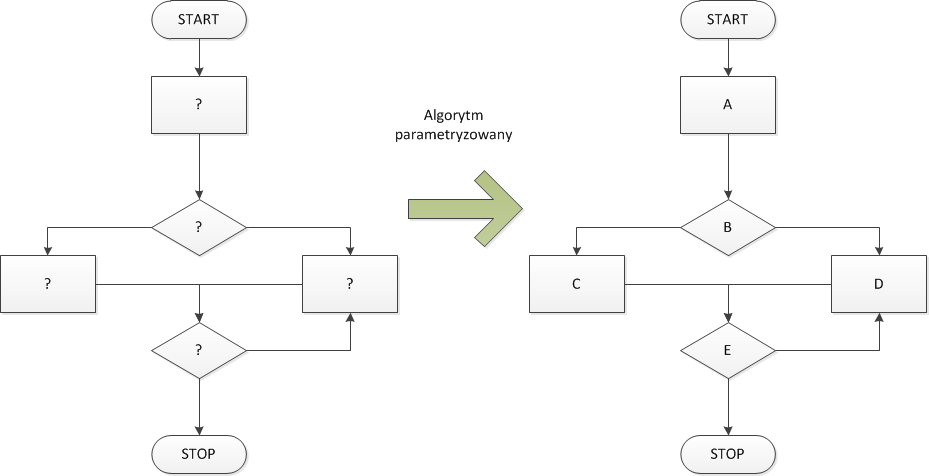
\includegraphics[width=.9\textwidth]{algorytmParametryzowany.png}}
    \caption{Algorytm parametryzowany~\cite{Cich07}}
    \label{rys:algorytmParametryzowany}
    \end{center}
\end{figure}

Reasumuj�c, definicja~\ref{def:definicjaUczenia} okre�la nam zmian� parametr�w jako wp�ywaj�c� na popraw� dzia�ania systemu~w~spos�b autonomiczny, podlegaj�c� procesowi uzupe�niania, korygowania~i~doskonalenia. Do zada� takiego systemu nale�y mi�dzy innymi~\cite{BolZar93}:
\begin{itemize}
\item "formu�owanie nowych poj��,
\item wykrywanie nieznanych dotychczas prawid�owo�ci~w~danych,
\item tworzenie regu� decyzyjnych,
\item przyswajanie nowych poj��~i~struktur drog� uog�lnienia przyk�ad�w~i~analogii,
\item modyfikowanie, uog�lnianie~i~precyzowanie danych,
\item zdobywanie wiedzy drog� konwersacji~z~lud�mi,
\item uog�lnianie obserwacji dokonanych sztucznymi zmys�ami,
\item generowanie wiedzy zrozumia�ej dla cz�owieka."
\end{itemize}

Docelowo zdolno�� do samodzielnego wnioskowania, jak� posiada cz�owiek, jest tym co chcemy osi�gn��~w~programie ucz�cym si�. Dodatkowo, chcemy aby komputery unika�y b��d�w charakterystycznych dla ludzi, kt�re wynikaj�~z~r�nych s�abo�ci cz�owieka jak np. zapominanie pewnych fakt�w niezb�dnych do podj�cia w�a�ciwej decyzji. Sam program powinien by� uniezale�niony od �rodowiska zewn�trznego. Jednak�e, aby osi�gn�� taki stan musimy wyposa�y� program~w~pocz�tkow� wiedz� poprzez dostarczenie odpowiedniej ilo�ci danych. Pozwoli to na ocen� dzia�ania programu~i~na pod��anie we w�a�ciwym kierunku. Oczywi�cie bierzemy pod uwag� pewn� �cis�� dziedzin�, aby nasze za�o�enia by�y realne~\cite{BolZar93}. Tak zdefiniowane programy postaramy si� opisa� ju� na konkretnych przypadkach wraz~z~dok�adniejszym om�wieniem~w~dalszych rozwa�aniach.

%---------------------------------------------------------------------------
%---------------------------------------------------------------------------

\subsection{Taksonomia uczenia maszynowego}
\label{sec:taksonomiaUczenia}

Postaramy si� teraz ukaza� faktyczny podzia� uczenia si� ze wzgl�du na r�ne kryteria klasyfikacji oraz wynikaj�cy~z~nich podzia� dziedziny na bardziej szczeg�owe obszary. W�r�d wspomnianych kryteri�w najbardziej znacz�ce s�~\cite{Cich07}:
\begin{description}
\item[Metoda reprezentacji wiedzy lub umiej�tno�ci] Wiele~w~tym przypadku zale�y od samej dziedziny zastosowania projektowanego systemu ucz�cego si�. Aby mo�liwe by�o efektywne operowanie na danych~z~dziedziny istnieje potrzeba wyboru pewnej reprezentacji danych, kt�ra maksymalizuje swoje zalety~i~minimalizuje wady~w~perspektywie tej dziedziny. Mo�emy tutaj wyr�ni� kilka~z~istniej�cych metod, takie jak drzewa decyzyjne, regu�y, rozk�ad prawdopodobie�stw czy automaty sko�czone.~W~zale�no�ci od wyboru mamy r�wnie� r�ny stopie� czytelno�ci danej reprezentacji dla cz�owieka, co te� jest pewnym czynnikiem wyboru~\cite{Mi83}\cite{Cich07}.~W~pracy skupimy si� na dw�ch metodach reprezentacji. Szczeg�owo na drzewach decyzyjnych oraz wspomnimy o regu�ach, kt�re w pewien spos�b s� powi�zane z struktur� drzew decyzyjnych.
\item[Spos�b u�ywania wiedzy lub umiej�tno�ci] Spos�b u�ywania wiedzy zale�y bezpo�rednio od wybranej metody reprezentacji wiedzy jak~i~przeznaczeniu wiedzy co jest powi�zane~z~zadaniem stawianym przed systemem. Najbardziej typowymi zadaniami s� klasyfikacja~i~aproksymacja. Celem klasyfikacji jest ustalenie przynale�no�ci pewnego bytu do konkretnej kategorii, natomiast celem aproksymacji jest odwzorowanie bytu na zbi�r liczb rzeczywistych\cite{Cich07}.~W~naszych rozwa�aniach skupiamy si� tylko~i~wy��cznie na klasyfikacji kt�ra okre�la cel postawiony~w~naszym problemie.
\item[�r�d�o~i~posta� informacji trenuj�cej]~W~tej cz�ci podzia� jest stosunkowo prosty. Uczenie dzielimy na uczenie nadzorowane (ang.~\emph{superviesed~learning}) oraz na uczenie nienadzorowane (ang.~\emph{unsupervised~learning}). Tak jak wida� na rysunku~\ref{rys:zrodloInformacjiTrenujacej}, proces ten polega na przetworzeniu pewnych danych wej�ciowych~i~wytworzeniu odpowiednich danych wyj�ciowych. Samo uczenie okre�la algorytm, kt�ry przetwarza dane, wytwarzaj�c oczekiwany rezultat. Dla \emph{uczenia nadzorowanego} �r�d�em informacji trenuj�cej jest \emph{nauczyciel}, kt�ry okre�la w�a�ciwe zachowania dla poszczeg�lnych danych. Natomiast dla \emph{uczenia nienadzorowanego} informacja taka jest niedost�pna~i~ucze� sam przetwarza dane decyduj�c~o~tym, jak nale�y to robi�\cite{Cich07}. Uczenie bez nadzoru jest stosowane g��wnie~w~metodzie uczenia maszynowego nazywanej grupowaniem, kt�ra wykracza poza temat pracy. Natomiast uczenie nadzorowane b�dzie towarzyszy�o nam do samego ko�ca pracy.

\begin{figure}[ht]
    \begin{center}
    \fbox{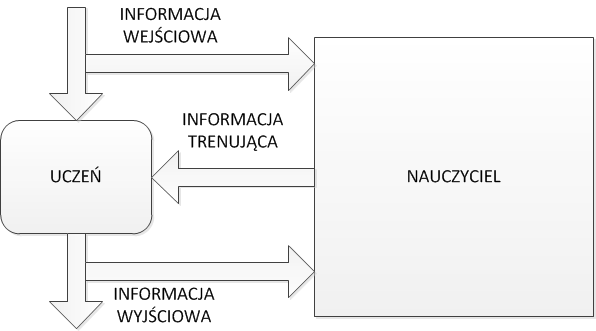
\includegraphics[width=.7\textwidth]{uczenZrodloInformacjiTrenujacej.png}}
    \caption{�r�d�o informacji trenuj�cej~\cite{Cich07}}
    \label{rys:zrodloInformacjiTrenujacej}
    \end{center}
\end{figure}

\item[Mechanizm nabywania~i~doskonalenia wiedzy lub umiej�tno�ci] Zdecydowanie najcz�ciej stosowanym mechanizmem jest indukcja. Polega ona na uog�lnianiu informacji trenuj�cej~w~celu uzyskania uog�lnionej wiedzy.~Z~drugiej strony mamy mechanizmy uczenia nieindukcyjnego.~W~tym przypadku celem jest konkretyzacja wiedzy ucznia na podstawie uog�lnionej trenuj�cej informacji~\cite{Cich07}.~W~naszej pracy b�dziemy si� skupia� na mechanizmie indukcji.

\end{description}

%---------------------------------------------------------------------------

\section{Indukcyjne uczenie si� }
\label{sec:indukcyjneUczenie}

Ca�y podrozdzia� jest po�wi�cony uczeniu si�~w~oparciu~o~wnioskowanie indukcyjne. Jednocze�nie rozdzia� ten jest wst�pem do dalszych rozwa�a�~o~praktycznych algorytmach, kt�re maj� zastosowanie~w~rozwi�zywaniu problem�w klasyfikacji.~W~podrozdziale zostanie opisana istota indukcyjnych mechanizm�w wnioskowania, kt�ra prowadzi do wyszukiwania hipotez najlepiej wyja�niaj�cych~i~uog�lniaj�cych obserwowane fakty, kt�re~w~tym przypadku nazywane s� przyk�adami. Rozdzia� ten zosta� stworzony na podstawie drugiego rozdzia�u ksi��ki Paw�a Cichosza~\cite{Cich07}. 



%---------------------------------------------------------------------------
%---------------------------------------------------------------------------

\subsection{Wnioskowanie indukcyjne}
\label{sec:wnioskowanieIndukcyjne}

Pierwsze wzmianki na temat indukcyjnego uczenia si� mo�na znale�� w pionierskich badaniach Hunta, Marina i Stone'a~\cite{Hun66} z lat sze��dziesi�tych. Wnioskowanie indukcyjne mo�na okre�li� jako stosowanie wstecz nast�puj�cej regu�y logicznej konsekwencji~\cite{Cich07}:
\begin{equation}
 P \wedge~W~\models K,
\end{equation}
w kt�rej kolejne symbole oznaczaj�: W~-~wiedza wrodzona ucznia, kt�ra mo�e by� pusta,~K~-~otrzymana~informacja trenuj�ca oraz P~-~wiedza powsta�a~w~wyniku procesu uczenia si�. Zar�wno jak~w~ksi��ce~\cite{Cich07} przyjmiemy pewne wygodne za�o�enia. B�dziemy oznacza� K jako T, czyli informacja \emph{trenuj�ca} oraz zamiast P b�dziemy pisa� h~w~celu oznaczenia hipotezy otrzymanej przez ucznia. Po naszych zmianach, regu�a logiczna wygl�da nast�puj�co:
\begin{equation}
 h \wedge~W~\models T.
\end{equation}
Mo�na zatem stwierdzi�, �e informacja trenuj�ca zdobyta przez ucznia jest logiczn� konsekwencj� jego wiedzy wrodzonej~W~oraz wygenerowanej przez niego hipotezy h. Innymi s�owy, informacja trenuj�ca zosta�a wyja�niona dzi�ki wrodzonej wiedzy ucznia oraz dzi�ki indukcyjnej hipotezie. Zak�adamy oczywi�cie �e powy�sze za�o�enie jest prawdziwe jak~i~jego wynik gdy wiedza wrodzona, hipoteza~i~informacja trenuj�ca s� poprawne. Niestety~w~praktycznych zastosowaniach cz�sto nale�y p�j�� na pewne ust�pstwa~i~zgodzi� si� na przybli�on� konsekwencj�~\cite{Cich07}.

Znalezienie poprawnej hipotezy polega na wykryciu~w~informacji trenuj�cej pewnych prawid�owo�ci, kt�re wraz~z~wiedz� wrodzon� pozwalaj� je~w~okre�lony spos�b wyt�umaczy�. Prowadzi to do przedstawienia wnioskowania indukcyjnego jako przechodzenia od fakt�w~i~obserwacji jednostkowych, kt�re~w~uczeniu si� nazywamy przyk�adami trenuj�cymi, do uog�lnie� czyli pewnej hipotezy stanowi�cej uog�lnienie przyk�ad�w trenuj�cych~\cite{Cich07}. Hipoteza opr�cz g��wnego celu jakim jest poprawne lub~w~przybli�eniu poprawne wyja�nianie informacji trenuj�cej powinna prowadzi� przede wszystkim do predykcji, czyli do przewidywania nowych fakt�w~i~obserwacji.~W~tym momencie mo�na wyr�ni� trzy podstawowe odmiany indukcyjnego uczenia si�: uczenie si� poj��, tworzenie poj�� oraz uczenie si� aproksymacji~\cite{Cich07}. Tak jak wcze�niej wspominali�my,~w~samej pracy skupiamy si� tylko na uczeniu si� poj�� czyli sposobie klasyfikacji. Reszta odmian indukcyjnego uczenia si� wykracza poza zakres pracy.

%---------------------------------------------------------------------------
%---------------------------------------------------------------------------

\subsection{Uczenie si� poj��}
\label{sec:uczenieSiePojec}

W indukcyjnym uczeniu si�, pozyskiwana przez ucznia wiedza stanowi pewne odwzorowanie otrzymanej informacji wej�ciowej na pewien zbi�r warto�ci wyj�ciowych. Informacje wej�ciow� s� opisy obiekt�w pewnej dziedziny. Nasze rozwa�ania~w~tym podrozdziale zaczniemy od zdefiniowania, jak� posta� takie opisy mog� przyjmowa�. 

\begin{quotation}
Definicje zosta�y zaczerpni�te z ksi��ki Paw�a Cichosza~\cite{Cich07}:

\begin{description}
\item[Dziedzina.] Dziedzin� nazywa� b�dziemy zbi�r obiekt�w oznaczany jako $X$, kt�rych dotyczy� ma wiedza nabywana przez ucznia. Mog� to by� osoby, sytuacje, stany rzeczy oraz cokolwiek innego, co stanowi argument odwzorowania, kt�rego nauczy� si� ma ucze�~\cite{Cich07}.
\item[Przyk�ady.] Ka�dy obiekt, element dziedziny $x \in X$, b�dziemy nazywa� przyk�adem~\cite{Cich07}.
\item[Atrybuty.] B�dziemy zak�ada�, �e przyk�ady s� opisywane za pomoc� atrybut�w. Atrybutem b�dziemy nazywa� dowoln� funkcj� okre�lon� na dziedzinie. Przyjmujemy, �e opis ka�dego przyk�adu $x \in X$ sk�ada si�~z~warto�ci $n \geq 1$ atrybut�w, $a_{1} \colon X \mapsto A_{1}, a_{2} \colon X \mapsto A_{2}, \dots, a_{n} \colon X \mapsto A_{n}$. Zbi�r wszystkich okre�lonych na rozwa�anej dziedzinie atrybut�w b�dziemy oznacza� przez $\mathbb{A} = \{a_{1},a_{2},\dots,a_{n}\}$~i~nazywa� zestawem lub \emph{przestrzeni� atrybut�w}.~W~praktyce czasem uto�samia si� przyk�ad $x$~z~wektorem warto�ci jego atrybut�w $\langle a_{1}(x),a_{2}(x),\dots,a_{n}(x) \rangle$, czyli przyk�adem nazywa si� dowolny element iloczynu kartezja�skiego przeciwdziedzin atrybut�w $A_{1} \times A_{2} \times \dots \times A_{n}$.~W~zale�no�ci od przeciwdziedziny (zbioru warto�ci) atrybuty dzieli si� na kilka typ�w:

\begin{itemize}
\item \textbf{nominalne}:~o~sko�czonym zbiorze nieuporz�dkowanych warto�ci dyskretnych,
\item \textbf{porz�dkowe}:~o~przeliczalnym zbiorze uporz�dkowanych warto�ci dyskretnych,
\item \textbf{ci�g�e}:~o~warto�ciach ze zbioru liczb rzeczywistych.
\end{itemize}
\end{description}

Dla dowolnego zbioru przyk�ad�w $P \subseteq X$, atrybutu $a \colon X \mapsto A$~i~jego warto�ci $v \in A$ oznaczamy przez $P_{av}$ zbi�r tych przyk�ad�w~z~$P$, dla kt�rych atrybut $a$ ma warto�� $v$, czyli $P_{av} = \{x \in P\ |\ a(x) = v\}$~\cite{Cich07}.

\end{quotation}

\begin{sample}
\label{prz:Pogoda}
Dziedzin� naszych rozwa�a� b�d� stany pogody. Ka�dy obiekt dziedziny b�dzie zawiera� atrybuty~\cite{Cich07}:
\begin{description}
\item[aura] atrybut nominalny, warto�ci: s�oneczna, pochmurna, deszczowa,
\item[temperatura] atrybut porz�dkowy, warto�ci: zimna umiarkowana, ciep�a,
\item[wilgotno��] atrybut porz�dkowy, warto�ci: normalna, du�a,
\item[wiatr] atrybut porz�dkowy, warto�ci: s�aby, silny.
\end{description}
\end{sample}

Poj�cia to jeden ze sposob�w opisu wiedzy~o~�wiecie. U�ywamy ich do opisywania oraz interpretowania zmys�owych obserwacji~i~abstrakcyjnych idei. Przyk�adowo, poj�cie samochodu osobowego pozwala rozr�nia� nam osobowe modele po�r�d innych pojazd�w, takich jak ci�ar�wki, motocykle czy rowery. Mo�emy sobie r�wnie� wyobrazi� wiele innych poj�� towarzysz�cych nam na co dzie�, kt�re pozwalaj� nam klasyfikowa� obiekty~z~tej samej dziedziny~\cite{Cich07}.

W najprostszym przypadku poj�cie mo�na zdefiniowa� jako podzia� zbioru wszystkich obiekt�w~z~danej dziedziny na dwie kategorie: obiekty nale��ce do danego poj�cia oraz te, kt�re do niego nie nale��. Jednak�e zdecydowanie cz�ciej stosowane jest \emph{poj�cie~wielokrotne}. Poj�cie wielokrotne dzieli dziedzin� na wiele kategorii,~z~kt�rych ka�da odpowiada jednemu~z~poj�� pojedynczych~\cite{Cich07}.~W~dalszej cz�ci pracy b�dziemy traktowa� poszczeg�lne poj�cia jako funkcje przekszta�caj�ce dziedzin�~w~zbi�r kategorii. Dodatkowo, b�dziemy m�wi�, �e poj�cie przypisuje \emph{etykiet�} kategorii danemu obiektowi~\cite{Cich07}.

Przyk�ady trenuj�ce s� z�o�one~z~dw�ch cz�ci: opis obiektu oraz etykieta kategorii. Przyk�adem \emph{nieetykietowanym} b�dziemy nazywa� przyk�ad, kt�ry posiada sam opis obiektu. Natomiast poprzez dodanie do przyk�adu nieetykietowanego etykiety kategorii otrzymujemy przyk�ad etykietowany. W�wczas, celem ucznia b�dzie znalezienie odpowiedniej etykiety dla przyk�adu nieetykietowanego na podstawie wiedzy wrodzonej~i~otrzymanej informacji trenuj�cej. Same przyk�ady trenuj�ce b�d� oczywi�cie przyk�adami etykietowanymi, dostarczaj�c pe�nej informacji na temat przyk�ad�w~\cite{Cich07}.

\begin{quotation}
Definicje zosta�y zaczerpni�te z ksi��ki Paw�a Cichosza~\cite{Cich07}: \\

\textbf{Poj�cia.} Zak�adamy, �e na dziedzinie mo�e by� okre�lona pewna klasa poj��, oznaczana przez~$\mathbb{C}$. Ka�de poj�cie $c \in \mathbb{C}$ jest funkcj� $c \colon X \mapsto C$, przy czym~$C$~oznacza sko�czony zbi�r kategorii poj�� klasy~$\mathbb{C}$.~W~przypadku poj�� pojedynczych b�dziemy przyjmowa� $C = \{0,1\}$.~W~przypadku poj�� wielokrotnych~$C$~mo�e by� dowolnym sko�czonym zbiorem kategorii~o~liczno�ci $|C| > 2$. Poj�cie pojedyncze wyznacza podzbi�r dziedziny, zawieraj�cy przyk�ady pozytywne tego poj�cia: $X^{C} = \{x \in X\ |\ c(x) = 1\}$. Pozosta�e elementy dziedziny s� przyk�adami negatywnymi poj�cia.~W~og�lnym przypadku dla kategorii $d \in C$, pewnego poj�cia~$c$~i~dowolnego zbioru przyk�ad�w $P \subseteq X$ przyjmujemy oznaczenie~$P^{cd}$~dla tych przyk�ad�w~z~$P$, kt�re nale�� do kategorii~$d$, czyli $P^{cd} = \{x \in P\ |\ c(x) = d\}$. Mo�liwe jest te� za�o�enie, �e~$c$~jest ustalonym poj�ciem docelowym.~W~tym przypadku pomijamy~$c$~i~piszemy $P^{d}$~\cite{Cich07}.

\begin{sample}
Dla dziedziny stan�w pogody z przyk�adu~\ref{prz:Pogoda} rozwa�my klas� poj��~$\mathbb{C}$~z�o�on� ze wszystkich mo�liwych poj�� pojedynczych. Przyk�adowym poj�ciem mo�e by� s�oneczny, ciep�y dzie�~o~du�ej wilgotno�ci~i~s�abym wietrze.
\end{sample}

\textbf{Hipotezy do uczenia si� poj��.} Dla danej dziedziny i klasy poj�� jest okre�lona, zale�na od stosowanego algorytmu uczenia si�, przestrze� mo�liwych hipotez, kt�r� b�dziemy oznacza�~$\mathbb{H}$. Przestrze� hipotez zawiera wszystkie hipotezy, jakie mo�e skonstruowa� ucze�. Ka�da hipoteza $h \in \mathbb{H}$, podobnie jak ka�de poj�cie, jest funkcj� przypisuj�c� przyk�adom ich kategorie,~a~wi�c mo�emy zapisa� $h\colon X \mapsto C$. Wynikiem uczenia si� poj�� jest zawsze wyb�r pewnej hipotezy z przestrzeni~$\mathbb{H}$, uznanej przez ucznia za najlepsz� na podstawie przyk�ad�w trenuj�cych i ewentualnie wiedzy wrodzonej. Dok�adne nauczenie si� ka�dego poj�cia docelowego $c \in \mathbb{C}$ jest mo�liwe tylko pod warunkiem, �e $\mathbb{C} \subseteq \mathbb{H}$. W�wczas wiadomo, �e $c \in \mathbb{H}$, czyli przestrze� hipotez zawiera hipotez� identyczn� z poj�ciem docelowym. W praktyce dla niekt�rych algorytm�w zachodzi niestety $\mathbb{H} \subset \mathbb{C}$~i~wtedy nie ma pewno�ci, �e uda si� dok�adnie nauczy� si� poj�cia docelowego~\cite{Cich07}.

W przypadku hipotez dla pojedynczych poj��, b�dziemy m�wi�, �e hipoteza \emph{pokrywa} przyk�ad je�li zosta� sklasyfikowany jako przyk�ad pozytywny, oraz dla przyk�adu negatywnego b�dziemy m�wi� �e hipoteza \emph{nie pokrywa} danego przyk�adu. Przez $P^{h}$ mo�emy oznaczy� w�wczas zbi�r przyk�ad�w~z~$P$~pokrywanych przez hipotez�~$h$.~W~og�lnym przypadku dla hipotezy $h\colon X \mapsto C$ przyjmujemy oznaczenie $P^{hd}$ dla zbioru przyk�ad�w~z~$P$, kt�rym hipoteza~$h$~przypisuje kategori� $d \in C$~\cite{Cich07}.

\begin{sample}
Dla dziedziny z przyk�adu~\ref{prz:Pogoda} rozwa�my przestrze� hipotez~$\mathbb{H}$~zawieraj�c� wszystkie hipotezy, kt�re mog� by� reprezentowane przez funkcje odwzorowuj�ce warto�ci atrybut�w, $|\mathbb{H}| = 2^{3*3*2*2} = 68719476736$.~W~tym przypadku najbardziej naturalne wydaje si� przyj�cie, �e dziedzina jest niesko�czona.~Z~tego wynika nam, �e $\mathbb{H} \subset \mathbb{C}$.
\end{sample}

\textbf{Zapytania do uczenia si� poj��.} Ka�da hipoteza b�d�ca rezultatem procesu uczenia si� poj�� mo�e by� zastosowana do klasyfikowania przyk�ad�w z dziedziny. \emph{Zapytaniem} nazywamy zg�oszenie przyk�adu, dla kt�rego za pomoc� danej hipotezy nale�y wyznaczy� kategori�. Klasyfikacja tego przyk�adu jest odpowiadaniem na zapytanie zadane uczniowi, kt�ry na podstawie najlepszej jego zdaniem hipotezy klasyfikuje przyk�ady~\cite{Cich07}.

\textbf{Informacja trenuj�ca do uczenia si� poj��.} Przyk�adem etykietowanym poj�cia~$c$~ okre�lonego na dziedzinie~$x$~b�dziemy nazywa� par� z�o�on� z nieetykietowanego przyk�adu $x \in X$~i~jego kategorii, kt�r� zapisujemy $\langle x,c(x) \rangle$. Zbiorem trenuj�cym do uczenia si� poj�cia docelowego~$c$~nazwiemy dowolny zbi�r etykietowanych przyk�ad�w tego poj�cia dostarczony uczniowi przez nauczyciela, opisanych za pomoc� atrybut�w okre�lonych na dziedzinie. Dla tak rozumianego zbioru trenuj�cego b�dziemy stosowa� oznaczenie $\langle T \rangle^{c}_{\mathbb{A}}$~i~definiowa� go~w~formalnie �cis�y spos�b nast�puj�co~\cite{Cich07}:
\begin{equation}
 \langle T \rangle^{c}_{\mathbb{A}} = \{\langle\langle x\rangle_{\mathbb{A}}, c(x)\rangle\ |\ x\ \in\ T\ \subseteq\ X\}.
\end{equation}
W dalszej cz�ci pracy b�dziemy zak�ada�, �e zbi�r trenuj�cy~$T$~zawiera przyk�ady~w~postaci wektor�w warto�ci atrybut�w,~a~etykiety kategorii s� r�wnie� dost�pne.

\begin{sample}
Dla dziedziny stan�w pogody z przyk�adu~\ref{prz:Pogoda} zbi�r trenuj�cy dla pewnego poj�cia docelowego przedstawia tabela~\ref{tab:zbiorTrenujacyPogoda}~\cite{Quin86}. Zbi�r danych przedstawiony w tej tabeli pos�u�y nam wielokrotnie przy omawianiu konkretnych algorytm�w uczenia maszynowego~i~przy analizie ich dzia�ania. Poj�cie okre�la, czy warunki pogodowe s� odpowiednie do gry w golfa. Poj�cie zawiera 9 pozytywnych i 5 negatywnych przyk�ad�w.
\end{sample}

\textbf{Niepoprawne dane trenuj�ce.} Problemem,~o~kt�rym ju� wcze�niej wspominali�my s� niepoprawne dane trenuj�ce. Nieprawid�owo�ci mog� objawia� si� zar�wno w opisie obiektu jako nieprawdziwe atrybuty lub w postaci �le przypisanej etykiecie kategorii. Niepoprawne dane trenuj�ce maj� r�ny wp�yw na r�ne algorytmy. Warto zauwa�y�, �e podstawowa definicja zbioru trenuj�cego zak�ada jego pe�n� poprawno��. O zbiorach trenuj�cych zawieraj�cych nieprawid�owe dane b�dziemy m�wi�, �e s� \emph{zaszumione}~\cite{Cich07}.

\textbf{B��d w uczeniu si� poj��.} B��d w uczeniu si� poj�� charakteryzuje stopie� zgodno�ci klasyfikacji przyk�ad�w przez poj�cie docelowe i hipotez� ucznia. Por�wnuj�c hipotez�~$h$~z~poj�ciem docelowym~$c$~na pewnym zbiorze przyk�ad�w $P \subseteq X$ mo�emy oszacowa� jej \emph{b��d pr�bki} jako stosunek liczby niepoprawnie klasyfikowanych przyk�ad�w~z~tego zbioru do liczby wszystkich jego element�w:
\begin{equation}
 	e^{c}_{P}(h) = \frac{|\{x\ \in\ P\ |\ h(x)\ \neq\ c(x)\}|}{|P|}.
\end{equation}

Wygodnie r�wnie� b�dzie pos�ugiwa� si� poni�szym wzorem dla licznika powy�szego u�amka, czyli liczby pomy�ek hipotezy~$h$~wzgl�dem poj�cia~$c$~na zbiorze~$P$:
\begin{equation}
	r^{c}_{P}(h) = |\{x\ \in\ P\ |\ h(x)\ \neq\ c(x)\}|.
\end{equation}

Zdecydowanie bardziej interesuj�ca dla nas jest warto�� \emph{b��du rzeczywistego} hipotezy, kt�ry mo�na interpretowa� jako oczekiwany b��d pr�bki na losowo wybranym zbiorze przyk�ad�w. Zak�adaj�c, �e przyk�ady s� wybierane~z~dziedziny zgodnie z okre�lonym na niej pewnym rozk�adem prawdopodobie�stwa~$\Omega$, definicj� b��du rzeczywistego mo�na zapisa� nast�puj�co:
\begin{equation}
 e^{c}_{\Omega}(h) = Pr_{x \in \Omega}(h(x) \neq c(x)),
\end{equation}
przy czym $Pr_{x \in \Omega}$ oznacza prawdopodobie�stwo przy za�o�eniu wylosowania~$x$~ze zbioru~$X$~zgodnie~z~rozk�adem~$\Omega$~\cite{Cich07}.

\textbf{Zadanie indukcyjnego uczenia si� poj��.} Zak�adamy, �e dane s� dziedzina~$X$, klasa poj��~$\mathbb{C}$~i~przestrze� hipotez ucznia~$\mathbb{H}$~oraz jest ustalone nieznane poj�cie docelowe $c \in \mathbb{C}$. Ucze�, maj�c dany zbi�r trenuj�cy $T \subseteq X$ dla poj�cia~$c$, ma znale�� hipotez� $h \in \mathbb{H}$, kt�ra jest najlepszym przybli�eniem poj�cia docelowego~$c$~wed�ug pewnego kryterium. Kryterium to na og� uwzgl�dnia minimalizacj� b��du pr�bki na zbiorze trenuj�cym $e^{c}_{T}(h)$, ale cz�sto nie ogranicza si� do niej. Je�li dany jest tak�e pewien rozk�ad prawdopodobie�stwa~$\Omega$~na dziedzinie~$X$~i~zbi�r trenuj�cy zawiera przyk�ady wybrane zgodnie~z~tym rozk�adem, to po��dany jest wyb�r hipotezy $h \in \mathbb{H}$ minimalizuj�cej b��d rzeczywisty $e^{c}_{\Omega}(h)$.~W~przypadku idealnym dok�adnego uczenia si� hipoteza jest identyczna~z~poj�ciem docelowym, czyli $(\forall x \in X)\ h(x) = c(x)$~\cite{Cich07}.

\end{quotation}

\begin{table}[!htbp]
\caption{Zbi�r trenuj�cy dla dziedziny stan�w pogody~\cite{Cich07}}
\label{tab:zbiorTrenujacyPogoda}
\begin{center}

	\begin{tabular}{| c || l | l | l | l || c |}
	\hline 
	x & aura 		& temperatura	& wilgotno�� 	& wiatr & c(x) \\ \hline \hline
	1 & s�oneczna 	& ciep�a 		& du�a 			& s�aby & 0 \\ \hline
	2 & s�oneczna 	& ciep�a 		& du�a 			& silny & 0 \\ \hline
	3 & pochmurna 	& ciep�a 		& du�a 			& s�aby & 1 \\ \hline
	4 & deszczowa 	& umiarkowana 	& du�a 			& s�aby & 1 \\ \hline
	5 & deszczowa 	& zimna 			& normalna 		& s�aby & 1 \\ \hline
	6 & deszczowa 	& zimna 			& normalna 		& silny & 0 \\ \hline
	7 & pochmurna 	& zimna			& normalna 		& silny & 1 \\ \hline
	8 & s�oneczna 	& umiarkowana 	& du�a 			& s�aby & 0 \\ \hline
	9 & s�oneczna 	& zimna 			& normalna 		& s�aby & 1 \\ \hline
	10 & deszczowa & umiarkowana 	& normalna 		& s�aby & 1 \\ \hline
	11 & s�oneczna & umiarkowana 	& normalna 		& silny & 1 \\ \hline
	12 & pochmurna & umiarkowana 	& du�a 			& silny & 1 \\ \hline
	13 & pochmurna & ciep�a 		& normalna 		& s�aby & 1 \\ \hline
	14 & deszczowa & umiarkowana 	& du�a 			& silny & 0 \\ \hline
	\end{tabular}
\end{center}
\end{table}

%---------------------------------------------------------------------------
%---------------------------------------------------------------------------

\subsection{Tryby uczenia si�}
\label{sec:trybyUczeniaSie}

Wa�nym elementem dla algorytm�w uczenia si� jest spos�b dostarczania danych trenuj�cych. Niekt�re z nich dopuszczaj� kilka mo�liwych tryb�w, a niekt�re s� ograniczane do jednego szczeg�lnego przypadku. W tej cz�ci pracy postaramy si� przedstawi� trzy najwa�niejsze \emph{tryby uczenia si�}, tryb wsadowy, tryb inkrementacyjny oraz tryb epokowy.~W~praktycznej cz�ci pracy skupimy si� g��wnie na trybie wsadowym, wspominaj�c o trybie inkrementacyjnym.

\begin{description}
\item[Tryb wsadowy] Jest to podstawowy tryb uczenia si�. Nak�ada najmniejsze wymagania na algorytm,~w~zasadzie ka�dy algorytm, kt�ry mo�e wykorzysta� inny tryb, mo�e wykorzysta� r�wnie� tryb wsadowy.~W~trybie tym ucze� na samym pocz�tku otrzymuje ca�� informacj� trenuj�c�, na podstawie kt�rej opiera swoje p�niejsze dzia�anie. Kontakt z nauczycielem sprowadza si� jedynie do pocz�tkowego momentu dzia�ania ucznia podczas procesu uczenia (przy przekazywaniu wszystkich przyk�ad�w ucz�cych)~\cite{Cich07}.
\item[Tryb inkrementacyjny] W trybie inkrementacyjnym, ka�dy przyk�ad jest podawany uczniowi pojedynczo. Po ka�dym przetworzonym przyk�adzie, ucze� udoskonala swoj� hipotez�. Dodatkowo, w dowolnym momencie mo�na uzna� hipotez� za wystarczaj�co dobr� i zaprzesta� dalszego procesu uczenia. Uczenie to ze wzgl�du na sw�j charakter jest nazywane uczeniem \emph{na bie��co}. Najwi�ksz� przydatno�� algorytmy odnajduj�~w~przypadkach, gdzie brak jest~z~g�ry okre�lonego zbioru trenuj�cego na pocz�tku procesu uczenia si�~\cite{Cich07}.
\item[Tryb epokowy] Tryb epokowy jest~w~pewnym sensie po��czeniem dw�ch wy�ej wymienionych tryb�w. Jest on zorganizowany~w~tzw. \emph{epoki}.~W~ka�dej~z~nich przetwarzany jest pewien zbi�r danych trenuj�cych. Po zako�czeniu ka�dej epoki, hipoteza ucznia jest uaktualniana~\cite{Cich07}.
\end{description}

%---------------------------------------------------------------------------
%---------------------------------------------------------------------------

\subsection{Obci��enie indukcyjne}
\label{sec:obciazenieIndukcyjne}

Obci��enie indukcyjne okre�la w�a�ciwo�ci algorytmu, kt�re decyduj�~o~wyborze hipotezy~w~przypadku, gdy wiedza wrodzona~i~informacja trenuj�ca nie wystarczaj� do jej jednoznacznego wyznaczenia. Obci��enie indukcyjne mo�emy zdefiniowa� jako~\cite{Cich07}:
\begin{definition}
Obci��eniem algorytmu indukcyjnego uczenia si� b�dziemy nazywa� czynniki, kt�re decyduj�~o~wyborze jednej hipotezy spo�r�d zbioru hipotez dopuszczalnych ze wzgl�du na cel uczenia si�.
\end{definition}
Hipoteza indukcyjna jest logiczn� konsekwencj� wiedzy wrodzonej, informacji trenuj�cej i obci��enia. Obci��enie cz�sto zale�y od za�o�e� jakie przyjmuje algorytm, dlatego przy analizach algorytm�w dodatkowo skupimy si� na obci��eniu indukcyjnym zwi�zanym~z~danym algorytmem uczenia maszynowego~\cite{Cich07}.~W~pracy Hausslera~\cite{Hauss88} znajdziemy obszerne informacje na temat obci��enia indukcyjnego.

%---------------------------------------------------------------------------

\section{Indukcja drzew decyzyjnych}
\label{sec:indukcjaDrzewDecyzyjnych}

Drzewa decyzyjne s� jedn� z najbardziej znanych i najszerzej praktycznie u�ywanych metod uczenia maszynowego. Algorytmy te pozwalaj� przybli�a� funkcje operuj�ce na dyskretnych warto�ciach dla kt�rych wynikiem jest poj�cie odpowiadaj�ce pewnej kategorii~\cite{Mit97}. Poni�szy rozdzia� opisuje t� metod� uczenia maszynowego. Aktualnie mo�na znale�� wiele praktycznie wykorzystywanych i popularnych algorytm�w indukcji drzew decyzyjnych, takie jak ID3~\cite{Quin86}, CART~\cite{Brei84}, ASSISTANT~\cite{Kono84} czy C4.5~\cite{Quin93}.

%---------------------------------------------------------------------------
%---------------------------------------------------------------------------

\subsection{Reprezentacja drzewa decyzyjnego}
\label{sec:reprezentacjaDrzewaDecyzyjnego}

Drzewo decyzyjne sk�ada si� z \emph{korzenia}, w�z��w przechowuj�cych testy, li�ci przechowuj�cych kategorie oraz kraw�dzi ��cz�cych wymienione elementy. Testy w w�z�ach sprawdzaj� warto�ci atrybut�w przyk�ad�w. Na podstawie wyniku testu prowadz� albo do innego w�z�a albo do li�cia. Dzi�ki takiej reprezentacji danych mo�emy przedstawi� dowolne hipotezy z dziedziny problemu~\cite{Kraw04}. Formalny opis drzewa odnajdziemy~w~ ksi��ce~\cite{Cich07}: drzewo okre�la si� jako dowolny sp�jny skierowany graf acykliczny, przy czym kraw�dzie takiego grafu, s� nazywane w�z�ami, a pozosta�e wierzcho�ki - li��mi. Dodatkowo przyjmuje si�, �e w grafie istnieje tylko jedna �cie�ka mi�dzy r�nymi wierzcho�kami. Id�c dalej, definicje struktury drzewiastej mo�emy przedstawi� w spos�b rekurencyjny~\cite{Cich07}:
\begin{definition}
Za��my, �e dana jest dziedzina~$C$, na kt�rej s� okre�lone atrybuty $a_{1},a_{2},\dots,a_{n}$ oraz klasa poj��~$\mathbb{C}$~o~zbiorze kategorii~$C$.
\begin{enumerate}
\item Li�� zawieraj�cy dowoln� etykiet� kategorii $d \in C$ jest drzewem decyzyjnym.
\item Je�li $t\ \colon\ X \mapsto R_{t}$ jest testem przeprowadzonym na warto�ciach atrybut�w przyk�ad�w~o~zbiorze mo�liwych wynik�w $R_{t} = \{r_{1},r{2},\dots,r_{m}\}$ oraz $\mathbb{T}_{1},\mathbb{T}_{2},\dots,\mathbb{T}_{m}$ s� drzewami decyzyjnymi, to w�ze� zawieraj�cy test~$t$,~z~kt�rego wychodzi~$m$~ga��zi, przy czym dla $i = 1,2,\dots,m$ ga��� $i$-ta odpowiada wynikowi $r_{i}$ i prowadzi do drzewa $\mathbb{T}_{i}$, jest drzewem decyzyjnym.
\end{enumerate}
\end{definition}

Test zawierany przez w�ze� jest funkcj� na atrybutach przyk�adu odwzorowuj�c� go na zbi�r wynik�w testu. W szczeg�lnych przypadkach wynikiem testu jest kategoria, co prowadzi bezpo�rednio do li�cia zawieraj�cego dan� kategori�. Mo�emy teraz zapisa� definicj� bazuj�c na ksi��ce~\cite{Cich07}. Je�li w�ze� zawiera test~$t$~ o zbiorze wynik�w $R_{t} = \{r_{1},r_{2},\dots,r_{m}\}$, a odpowiadaj�ce im ga��zie prowadz� do poddrzew $\mathbb{T}_{1},\mathbb{T}_{2},\dots,\mathbb{T}_{m}$, to hipotez� reprezentowan� przez ten w�ze� mo�na dla ka�dego przyk�adu $x \in X$ zapisa� nast�puj�co~\cite{Cich07}:

\begin{equation}
h(x)  =  \left\lbrace
\begin{array}{rcl}
\vspace*{7mm} h_{1}(x)  &  \mbox{je�li} & t(x)  =  r_{1},\\ 
\vspace*{7mm} h_{2}(x)  &  \mbox{je�li} & t(x)  =  r_{2},\\
\vspace*{7mm} \dots  &	\	& \ \\
h_{m}(x)  &  \mbox{je�li} &  t(x)  =  r_{m},\\
\end{array}
\right.
\end{equation}

\vspace*{1cm}
przy czym $h_{1},h{2},\dots,h_{m}$ s� odpowiednio hipotezami reprezentowanymi przez drzewa  $\mathbb{T}_{1},\mathbb{T}_{2},\dots,\mathbb{T}_{m}$.

Wyznaczenie klasy do kt�rej nale�y obiekt za pomoc� drzewa decyzyjnego polega na przej�ciu �cie�ki od korzenia drzewa do jednego z li�ci, poprzez przechodzenie przez kolejne testy w w�z�ach wzd�u� kraw�dzi drzewa~\cite{Cich07}. Ka�dy test dok�adnie opisuje w jaki spos�b dokonano podzia�u na podstawie warto�ci atrybut�w obiektu. Dodatkowo o drzewie m�wimy, �e jest drzewem \emph{klasyfikacyjnym}, je�li jest reprezentacj� podzia�u zbioru obiekt�w na jednorodne klasy~\cite{Gat98}. W dalszej cz�ci pracy b�dziemy w razie potrzeby oznacza� przez $N_{\mathbb{T}}$ zbi�r w�z��w drzewa decyzyjnego $\mathbb{T}$ oraz przez $L_{\mathbb{T}}$ zbi�r jego li�ci~\cite{Cich07}.

\begin{sample}
Dla dziedziny stan�w pogody z przyk�adu~\ref{prz:Pogoda} przyk�adowe drzewo decyzyjne znajduje si� na rysunku~\ref{rys:drzwewoDecyzyjneDlaPogody}. Decyzj�, kt�r� podejmujemy w tym przypadku jest gra w tenisa. Oczywi�cie, to czy zagramy zale�y od stanu pogody~\ref{tab:zbiorTrenujacyPogoda}. Przyk�ad zawiera trzy w�z�y, z kt�rych w�ze� \emph{aura} jest zarazem korzeniem drzewa. Li�cie reprezentuj� dwie kategorie, gramy w tenisa~(\emph{tak}) lub nie gramy w tenisa~(\emph{nie}). Dla obiektu s�oneczny, wilgotno�� normalna, wiatr silny otrzymujemy kategori� \emph{tak}. Pierwszym testem jest \emph{aura}, kt�ry przenosi nas poprzez kraw�d� \emph{s�oneczny} do w�z�a z testem \emph{wilgotno�ci}. W tym przypadku test \emph{wiatru} jest pomijany. Nast�pnie test \emph{wilgotno�ci} prowadzi nas do li�cia z kategori� \emph{tak}. Drzewo decyzyjne, podane w przyk�adzie, mo�emy r�wnie� przedstawia� w innych reprezentacjach. Poni�ej prezentujemy posta� tekstow� naszego drzewa:
\begin{lstlisting}
aura = deszczowa =>
	wiatr = silny => NIE
	wiatr = s�aby => TAK
aura = pochmurna => TAK
aura = s�oneczna =>
	wilgotno�� = du�a => NIE
	wilgotno�� = normalna => TAK
\end{lstlisting}
\end{sample}

\begin{figure}[ht]
    \begin{center}
    \fbox{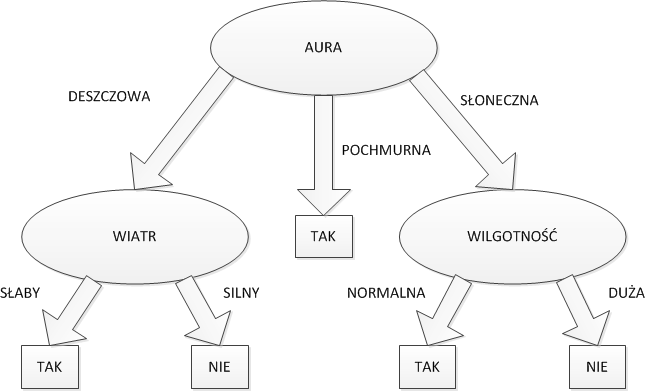
\includegraphics[width=.8\textwidth]{przykladoweDrzewoDecyzyjne.png}}
    \caption{Drzewo decyzyjne dla stan�w pogody}
    \label{rys:drzwewoDecyzyjneDlaPogody}
    \end{center}
\end{figure}

%---------------------------------------------------------------------------
%---------------------------------------------------------------------------

\subsection{Zalety i ograniczenia drzew decyzyjnych}
\label{sec:zaletyOgraniczeniaDrzew}

Drzewa decyzyjne posiadaj� wiele zalet, kt�rym zawdzi�czaj� swoj� popularno��. W zasadzie dowolne poj�cia pojedyncze i wielokrotne mog� by� reprezentowane przez drzewa decyzyjne, je�li tylko mo�na je zdefiniowa� za pomoc� atrybut�w u�ywanych do opisu przyk�ad�w. Dodatkowo, metoda ta cechuje si� do�� du�� efektywno�ci� pami�ciow� w por�wnaniu z innymi podej�ciami oraz pozwalaj� na efektown� implementacj� procesu klasyfikowania przyk�ad�w~\cite{Cich07}. Do tego nale�y zaznaczy�, �e dop�ki drzewo nie osi�gnie pewnego du�ego stopnia komplikacji, jest stosunkowo czytelne dla cz�owieka, co cz�sto nie pozostaje bez uwagi. Co wi�cej, mamy mo�liwo�� �atwego przej�cia do reprezentacji regu�owej, kt�rej czytelno�� dla cz�owieka jest co najmniej taka jak dla drzew decyzyjnych~\cite{Cich07}.

Z drugiej strony, z drzewami decyzyjnymi wi��� si� r�wnie� pewne ograniczenia. Po pierwsze, podstawowe algorytmy dzia�aj� tylko na atrybutach dyskretnych, przez co musimy dokonywa� dyskretyzacji wszelakich atrybut�w ci�g�ych. Oczywi�cie istniej� rozszerzenia tych algorytm�w, kt�re pozwalaj� pracowa� z atrybutami ci�g�ymi. Jednak wi��e si� to ze zwi�kszeniem stopnia skomplikowania samego algorytmu oraz cz�sto z utrat� wydajno�ci. R�wnie� testy pojedynczych atrybut�w nie pozwalaj� nam wyszukiwa� zale�no�ci mi�dzy r�nymi atrybutami. W tym przypadku r�wnie� istniej� rozszerzenia algorytm�w pozwalaj�ce radzi� sobie z t� niedogodno�ci�, ale r�wnie� tracimy na wydajno�ci algorytmu i komplikujemy samo rozwi�zanie problemu. Ostatni� rzecz� o kt�rej mo�na wspomnie�, jest inkrementacyjna aktualizacja, z kt�r� r�wnie� drzewa decyzyjne maj� problem~\cite{Cich07}. Dodatkowe informacje na ten temat mo�na znale�� w pozycji~\cite{Mit97} w rozdziale \emph{3.3}.

Tak naprawd�, to czy zalety lub ograniczenia wp�ywaj� na nasz wyb�r zale�y od samej domeny problemu. W przypadku rozwa�anym w pracy, czyli zarz�dzanie zadaniami w pewnej organizacji mamy do czynienia z danymi dyskretnymi. R�wnie� inkrementacyjna aktualizacja nie stanowi dla nas problemu ze wzgl�du na za�o�enie, �e mamy odpowiedni zbi�r danych ju� na  pocz�tku procesu uczenia si�. Dlatego warto ponownie zaznaczy�, �e poszczeg�lne wady i ograniczenia w r�ny spos�b oddzia�uj� na nasz wyb�r algorytmu do rozwi�zania problemu w zale�no�ci w�a�nie od jego dziedziny i innych szczeg��w.

%---------------------------------------------------------------------------
%---------------------------------------------------------------------------

\subsection{Algorytm indukcji drzew decyzyjnych - schemat og�lny}
\label{sec:algoytmyIndukcjiDrzewDecyzyjnychSchematOgolny}

W 1966 roku Hunt poda� algorytm CLS (ang. Concept Learning System)~\cite{Hun66}. Algorytm ten tworzy opis poj�cia w postaci drzewa decyzyjnego. Dalszym rozwini�ciem tego algorytmu by� algorytm ID3~\cite{Quin79}, kt�ry jest wykorzystywany jako podstawa algorytmu opracowanego w tej pracy. Oba algorytmy wykorzystuj� reprezentacj� przyk�ad�w domeny w postaci wektor�w w�asno�ci. Pocz�tkowym za�o�eniem by�o wykorzystanie tylko warto�ci dyskretnych we w�asno�ciach przyk�ad�w, co w p�niejszym czasie si� zmieni�o w kolejnych rozwini�ciach algorytmu ID3~\cite{BolZar93}. Drzewa reprezentuj� opisy poj��, w w�z�ach umieszczane s� testy, na wychodz�cych z nich ga��ziach - mo�liwe wyniki test�w, a w li�ciach - informacje o przynale�no�ci do konkretnych klas~\cite{BolZar93}.

Wi�kszo�� algorytm�w uczenia si� drzew decyzyjnych opiera si� na podobnym heurystycznym schemacie zst�puj�cego konstruowania drzewa (ang. TDIDT - Top Down Induction of Decision Trees). Rozwi�zanie to zosta�o u�yte ju� w pierwszych algorytmach, takich jak wspominany ID3~\cite{Quin79} czy CART~\cite{Brei84}. Spos�b wyboru testu dla w�z�a zwi�zanego z ocen� jako�ci podzia�u zbioru, techniki uwzgl�dniania r�nego rodzaju zaburze� w opisie przyk�ad�w ucz�cych to tylko niekt�re z r�nic mi�dzy konkretnymi algorytmami~\cite{Kraw04}.

Przedstawimy teraz podstawowy schemat zst�puj�cego konstruowania drzewa w oparciu o podstawowy algorytm ID3. Budowa drzewa rozpoczyna si� w od podj�cia decyzji, czy ma ono by� li�ciem czy w�z�em, oraz odpowiedniego wyboru etykiety kategorii w pierwszym przypadku lub testu w drugim przypadku. Gdy wybrany zosta� wariant z w�z�em, w�wczas poszczeg�lnym wynikom test�w odpowiadaj� ga��zie prowadz�ce z tego w�z�a do poddrzew skonstruowanych zgodnie z tym samym schematem~\cite{Mit97}~\cite{Cich07}.

Schemat ten najwygodniej zdefiniowa� w postaci procedury rekurencyjnej. Zak�adamy, �e otrzymuje ona jako argumenty zbi�r P etykietowanych przyk�ad�w poj�cia docelowego \emph{c}, dla kt�rych ma by� zbudowane drzewo, domy�ln� etykiet� kategorii \emph{d} przypisywan� tworzonemu li�ciowi, je�li w�a�ciwej etykiety nie mo�na okre�li� na podstawie zbioru \emph{P}, oraz zbioru test�w \emph{S}, jakie mog� by� u�yte w tworzonych w�z�ach. Algorytm zosta� przedstawiony w dalszej cz�ci pracy~\ref{lst:budujDrzewo}. Jest to oczywi�cie wy�ej wspomniany algorytm TDIDT. Operacja budowania drzewa dla zbioru trenuj�cego \emph{T} mo�e by� zapisana jako wywo�anie \emph{buduj-drzewo$(T, arg \max_{d} \left| T^{d} \right|, S)$} je�li przyjmiemy za domy�ln� etykiet� kategorii najliczniej reprezentowanej w zbiorze trenuj�cym~\cite{Cich07}.

O utworzeniu li�cia lub w�z�a w naszym algorytmie decyduje kryterium stopu. Je�li zosta�o spe�nione, tworzony jest li��~\textbf{l}~i~na podstawie etykietowanych przyk�ad�w ze zbioru \emph{P} ustalana jest jego etykieta $d_{l}$, na czym ko�czymy proces budowy drzewa. W przeciwnym wypadku tworzymy w�ze� \textbf{n} - dokonuje si� wyboru testu $t_{n}$ ze zbioru \emph{S}, a nast�pnie dla ka�dego z jego mo�liwych wynik�w odpowiednia ga��� w�z�a prowadzi do poddrzewa, kt�re jest budowane przez wywo�anie tej samej procedury rekurencyjnie. Ka�de wywo�anie rekurencyjne tworzy poddrzewo, do kt�rego ma prowadzi� ga��� odpowiadaj�ca wynikowi \emph{r} testu $t_{n}$. Dodatkowo, ka�de takie wywo�anie otrzymuje jako argument zbi�r przyk�ad�w zawieraj�cych wy��cznie te przyk�ady z \emph{P}, dla kt�rych test $t_{n}$ daje wynik \emph{r}. Zbi�r pozostaj�cych test�w \emph{S} jest pomniejszany o test $t_{n}$, gdy� jego ponowne zastosowanie na ni�szym poziomie drzewa nie przynosi �adnych korzy�ci~\cite{Cich07}.

Wyst�puj�ce w schemacie operacje \emph{kryterium-stopu, kategoria i wybierz-test} pozwalaj� na r�ne konkretyzacje algorytmu. W dalszej cz�ci zostan� opisane konkretne rozwi�zania realizuj�ce powy�sze operacje.

\lstset{emph={buduj-drzewo,kryterium-stopu,kategoria,wybierz-test}}

\begin{lstlisting}[name=BudujDrzewo, language=Pascal, caption={Schemat zst�puj�cego konstruowania drzewa decyzyjnego~\cite{Cich07}}, label={lst:budujDrzewo}]
function buduj-drzewo(P,d,S)
\end{lstlisting}
\textbf{Argumenty Wej�ciowe:}
\begin{enumerate}
\item P - zbi�r przyk�ad�w etykietowanych poj�cia c,
\item d - domy�lna etykieta kategorii,
\item S - zbi�r mo�liwych test�w;
\end{enumerate}
\textbf{Zwraca:} drzewo decyzyjne reprezentuj�ce hipotez� przybli�aj�c� \emph{c} na zbiorze \emph{P};

\begin{lstlisting}[name=BudujDrzewo, language=Pascal, frame = trBL, mathescape=true, otherkeywords={{l},{return}}]
if kryterium-stopu(P,S) then
	utw�rz li�� l;
	$d_{1}$ := kategoria(P,d);
	return l;
end if;
utw�rz w�ze� n;
$t_{n}$ := wybierz-test(P,S);
d := kategoria(P,S);

for $r \in R_{t_{n}}$ do
	n[r] := buduj-drzewo($P_{t_{n}r}, d, S - {t_{n}}$);
end for;

return n
\end{lstlisting}

%---------------------------------------------------------------------------
%---------------------------------------------------------------------------

\subsection{Realizacja schematu og�lnego}
\label{sec:realizacjaSchematuOgolnegoKryteriumStopu}

\subsubsection*{Kryterium stopu i ustalenie etykiety}

Ka�de rekurencyjne przej�cie algorytmu zaw�a nam liczb� przyk�ad�w analizowanych w kolejnych testach. Zag��biaj�c si� coraz dalej, liczba przyk�ad�w nadal si� zmniejsza a� do momentu kiedy wszystkie przyk�ady znajduj�ce si� w danym w�le nale�� do jednej kategorii lub zbi�r przyk�ad�w jest pusty. Widzimy tutaj najprostszy i zrazem naturalny warunek stopu. Warunek ten mo�e by� sformalizowany w nast�puj�cy spos�b~\cite{Cich07}:
\begin{equation}
	P = \emptyset \vee \left|~\{d' \in C~|~(\exists x \in P)~c(x) = d'\}~\right| = 1.
\end{equation}
W podanym r�wnaniu przez \emph{C} oznaczono zbi�r kategorii dla rozwa�anej klasy poj��. Dla dw�ch przypadk�w, kt�re s� rozwa�ane tworzymy li�cia. Gdy wszystkie przyk�ady nale�� do jednej kategorii, w�wczas przypisujemy li�ciowi t� kategorie. W przeciwnym przypadku, kiedy zbi�r przyk�ad�w jest pusty -- przypisujemy li�ciowi kategori� domy�ln�, czyli najcz�ciej kategorie najliczniej reprezentowan� przez zbi�r przyk�ad�w rozwa�anych we wcze�niejszym kroku algorytmu. W tym momencie mamy zdefiniowan� podstawow� wersj� operacji \emph{kategoria(P, d)}~\cite{Cich07}.

Dodatkowo mo�na za�o�y� pewne z�agodzenie warunku stopu, kt�re pozwoli wcze�niej nam zatrzyma� algorytm. Je�li dla pewnego problemu wystarczaj�ce jest aby wi�kszo�� przyk�ad�w nale�a�a do jednej kategorii gdy liczba przyk�ad�w spadnie poni�ej pewnego za�o�onego minimum, w�wczas mo�emy zdecydowa� si� na przypisanie tej kategorii jako warto�� li�cia. Jest to jedno z rozwi�za� stosowanych w celu unikni�cia nadmiernego dopasowania drzewa decyzyjnego do zbioru przyk�ad�w~\cite{Cich07}. Do problemu tego wr�cimy w dalszej cz�ci pracy.

\subsubsection*{Rodzaje test�w}

W naszej pracy wykorzystujemy wy��cznie testy dla atrybut�w nominalnych, dlatego te� opiszemy tylko ten rodzaj test�w. Innymi bardzo popularnymi testami s� testy dla atrybut�w porz�dkowych i ci�g�ych.

Zak�adamy, �e atrybuty posiadaj� warto�ci nominalne o sko�czonej, stosunkowo niewielkiej liczbie warto�ci. Stosowane testy s� dosy� proste, testujemy warto�� atrybutu. Mo�na to uj�� w spos�b formalny. Dla testu \emph{t} i atrybutu \emph{a}, takich �e $t~:~X \mapsto R_{t}, a~: X \mapsto A$ mamy $R_{t} = A$ oraz dla ka�dego $x \in X$ mamy $t(x) = a(x)$~\cite{Cich07}. Takie testy nazywamy testami \emph{to�samo�ciowymi}.

\subsubsection*{Kryterium wyboru testu}

Dochodzimy do g��wnego elementu algorytm�w drzew decyzyjnych -- wyboru testu. Od wyboru testu, czyli w naszym przypadku od wyboru atrybutu kt�ry testujemy i warunku, kt�ry musi spe�ni� zale�y jako�� dzia�ania samego drzewa decyzyjnego. Przy wyborze takiego testu na danym poziomie drzewa b�dziemy wykorzystywa� \emph{zysk informacyjny} (ang. information gain). Zysk informacyjny wskazuje jak du�� warto�� ma wykorzystanie danego atrybutu dziel�cego przyk�ady na podzbiory do dalszych test�w~\cite{Mit97}.

Najprostsz� i skuteczn� miar� spe�niaj�c� nasze wymagania jest \emph{entropia} (ang. entropy), kt�ra charakteryzuje czysto�� przyk�ad�w w danym zbiorze. Idea�em w tym przypadku jest zbi�r przyk�ad�w jednej kategorii, kt�ry jest zbiorem czystym z punktu widzenia entropii i osi�ga najkorzystniejsz� warto�� miary. Je�li we�miemy pod uwag� zbi�r przyk�ad�w \emph{S}, zawieraj�cy przyk�ady spe�niaj�ce pewien warunek i niespe�niaj�ce (binarna klasyfikacja), entropi� mo�emy zdefiniowa� w nast�puj�cy spos�b~\cite{Mit97}:

\begin{equation}
\label{eq:entropyBinary}
	Entropy(S) \equiv -p_{\varoplus} \log_{2} p_{\varoplus} - p_{\varominus} \log_{2} p_{\varominus},
\end{equation}

gdzie $p_{\varoplus}$ jest stosunkiem liczby przyk�ad�w spe�niaj�cych warunek do liczby wszystkich przyk�ad�w, a $p_{\varominus}$ jest stosunkiem przyk�ad�w niespe�niaj�cych warunku.

\begin{sample}
Przyk�adowo, S jest kolekcj� 20 element�w typu binarnego, gdzie 12 jest pozytywnych, a reszta negatywnych. W�wczas entropia wynosi:

$Entropy(12+,8-) = - (12/20)\log_{2}(12/20) - (8/20)\log_{2}(8/20) = 0,970$.
\end{sample}
Nale�y zwr�ci� uwag� na kilka aspekt�w powi�zanych z t� miar�. Gdy wszystkie przyk�ady nale�� do jednej kategorii, entropia wynosi 0. Gdy zbiory odpowiadaj�ce r�nym kategori� maj� te same liczby przyk�ad�w, entropia wynosi 1. W pozosta�ych przypadkach, warto�� entropii zawiera si� miedzy 0 i 1.

Jednak podana miara oczywi�cie jest niewystarczaj�ca. Potrzebujemy miary, kt�ra dla dowolnej liczby kategorii b�dzie wstanie wskaza� nam warto�� entropii. Dlatego b�dziemy korzysta� z bardziej og�lnej definicji~\cite{Mit97}:
\begin{equation}
\label{eq:entropy}
	Entropy(S) \equiv \sum_{i=1}^{C} - p_{i}\log_{2}p_{i}
\end{equation}
gdzie S jest zbiorem przyk�ad�w, \emph{i} jest kolejn� kategori� ze zbioru \emph{C}, a $p_{i}$ jest odpowiednim stosunkiem element�w kategorii \emph{i} do wszystkich element�w.

Maj�c jako narz�dzie mechanizm wyznaczania czysto�ci zbioru, mo�emy zdefiniowa� miar� \emph{zysku informacyjnego} opart� o definicj� og�ln� entropii. B�dziemy starali si� uzyska� oczekiwan� wysok� warto�� zysku informacyjnego poprzez partycjonowanie danych za pomoc� wyznaczania entropii dla ka�dego atrybutu. Najlepszy podzia� (najlepsza warto�� zysku informacyjnego) b�dzie nam wskazywa� najlepszy test, kt�ry powinien zosta� u�yty na danym poziomie drzewa decyzyjnego. Zysk informacyjny definiujemy nast�puj�co~\cite{Mit97}:
\begin{equation}
\label{eq:gainInformation}
	Gain(S,A) \equiv Entropy(S) - \sum_{v \in Values(A)} \frac{\left|S_{v}\right|}{\left|S\right|} Entropy(S_{v})
\end{equation}
gdzie $Values(A)$ jest zbiorem mo�liwych warto�ci atrybutu $A$ oraz $S_{v}$ jest podzbiorem przyk�ad�w $S$, kt�re posiadaj� odpowiedni� warto�� atrybutu $A$. Dodatkowo wykorzystujemy tu znan� nam miar� entropii, oraz stosunek liczby element�w zbioru $S_{v}$ i zbioru wszystkich element�w $S$ - $\frac{\left|S_{v}\right|}{\left|S\right|}$~\cite{Mit97}.

Poni�ej znajduje si� przyk�ad na podstawie danych z tabeli~\ref{tab:zbiorTrenujacyPogoda}. Sprawdzimy zysk informacyjny dla atrybut�w \emph{aura}, \emph{temperatura}, \emph{wilgotno��} i \emph{wiatr}.

\begin{sample}
\label{ex:zyskInformacyjny}
Zbi�r przyk�ad�w~\ref{tab:zbiorTrenujacyPogoda}, dane dla ca�ego zbioru: \textbf{S} = [9+,5-], \textbf{Entropy(S)} = 0.940 \\

\textbf{Zysk informacyjny dla atrybutu aura:} \\
Values(aura) = [s�oneczna, pochmurna, deszczowa] \\
$S_{sloneczna} = [2+,3-]$ \\
$S_{pochmurna} = [4+,0-]$ \\
$S_{deszczowa} = [3+,2-]$ 

\textbf{GAIN(S,aura)}~$= Entropy(S) - \sum_{v \in \{sloneczna,pochmurna,deszczowa\}} \frac{\left|S_{v}\right|}{\left|S\right|} Entropy(S_{v}) =$ \\
$=Entropy(S) - \frac{5}{14}Entropy(S_{sloneczna}) - \frac{4}{14}Entropy(S_{pochmurna}) - \frac{5}{14}Entropy(S_{deszczowa}) =$ \\
$=0,940 - \frac{5}{14}(0,970) - \frac{4}{14}(0) - \frac{5}{14}(0,970) = 0,247$ \\
\newline
\textbf{Zysk informacyjny dla atrybutu temperatura:} \\
Values(temperatura) = [ciep�a, umiarkowana, zimna] \\
$S_{ciepla} = [2+,2-]$ \\
$S_{umiarkowana} = [4+,2-]$ \\
$S_{zimna} = [3+,1-]$ 

\textbf{GAIN(S,temperatura)}~$= Entropy(S) - \sum_{v \in \{ciepla,umiarkowana,zimna\}} \frac{\left|S_{v}\right|}{\left|S\right|} Entropy(S_{v}) =$ \\
$=Entropy(S) - \frac{4}{14}Entropy(S_{ciepla}) - \frac{6}{14}Entropy(S_{umiarkowana}) - \frac{4}{14}Entropy(S_{zimna}) =$ \\
$=0,940 - \frac{4}{14}(1) - \frac{6}{14}(0,918) - \frac{4}{14}(0,811) = 0,029$ \\
\newline
\textbf{Zysk informacyjny dla atrybutu wilgotno��:} \\
Values(wilgotno��) = [du�a, normalna] \\
$S_{duza} = [3+,4-]$ \\
$S_{normalna} = [6+,1-]$ 

\textbf{GAIN(S,wilgotno��)}~$= Entropy(S) - \sum_{v \in \{duza,normalna\}} \frac{\left|S_{v}\right|}{\left|S\right|} Entropy(S_{v}) =$ \\
$=Entropy(S) - \frac{7}{14}Entropy(S_{duza}) - \frac{7}{14}Entropy(S_{normalna}) =$ \\
$=0,940 - \frac{7}{14}(0,985) - \frac{7}{14}(0,591) = 0,152$ \\
\newline
\textbf{Zysk informacyjny dla atrybutu wiatr:} \\
Values(wiatr) = [s�aby, silny] \\
$S_{slaby} = [6+,2-]$ \\
$S_{silny} = [3+,3-]$ 

\textbf{GAIN(S,wiatr)}~$= Entropy(S) - \sum_{v \in \{slaby,silny\}} \frac{\left|S_{v}\right|}{\left|S\right|} Entropy(S_{v}) =$ \\
$=Entropy(S) - \frac{8}{14}Entropy(S_{slaby}) - \frac{6}{14}Entropy(S_{silny}) =$ \\
$=0,940 - \frac{8}{14}(0,811) - \frac{6}{14}(1) = 0,048$ \\

Z oblicze� wynika, �e najlepszym atrybutem testowym w pocz�tkowej fazie tworzenia drzewa decyzyjnego jest atrybut aura, kt�rego zysk informacyjny jest najwy�szy~i~wynosi~$0,247$.
\end{sample}

Niestety algorytm ten ma pewn� wad�. Faworyzuje on atrybuty o dziedzinach wielowarto�ciowych wzgl�dem innych atrybut�w o niewielkiej liczbie warto�ci. W pewnych sytuacjach prowadzi to do niepotrzebnego i nadmiernego powi�kszania drzewa decyzyjnego (g��wnie wszerz). Algorytm ten zbytnio przywi�zuje si� do danych ucz�cych, przez co maleje jego korzy�� w sytuacjach og�lnych~\cite{Kraw04}. Dlatego, wykorzystamy inn� miar�, kt�ra niweluje t� wad�. Miar� tak� zaproponowa� Quinlan~\cite{Quin86}. Pomys� polega na karaniu atrybut�w o wielowarto�ciowych domenach, a sama miara nazywa si� \emph{podzia�em informaji} (ang. split information). Zdefiniowana jest w nast�puj�cy spos�b~\cite{Mit97}\cite{Quin86}:
\begin{equation}
	SplitInformation(S,A) \equiv - \sum_{i=1}^{C} \frac{\left|S_{i}\right|}{\left|S\right|} \log_{2} \frac{\left|S_{i}\right|}{\left|S\right|}
\end{equation}
gdzie $S_{i}$ jest podzbiorem S utworzonym podczas podzia�u przez warto�� atrybutu A odpowiedni� dla danej kategorii \emph{i}. Dzi�ki tak zdefiniowanej mierze, mo�emy p�j�� krok dalej i zapisa� now� miar� zysku informacyjnego, kt�r� b�dziemy nazywa� ilorazem przyrostu informacji (ang. gain ratio)~\cite{Quin86}:
\begin{equation}
\label{eq:gainRatio}
	GainRatio(S,A) \equiv \frac{Gain(S,A)}{SplitInformation(S,A)}
\end{equation}
Miara ta dokonuje normalizacji warto�ci, przez co znika bezzasadne faworyzowanie wielowarto�ciowych atrybut�w. R�wnie� w tym przypadku, atrybut kt�ry uzyska najwy�sz� warto�� naszej miary, b�dzie atrybutem preferowanym do utworzenia testu na aktualnym poziomie drzewa, dla przyk�ad�w \emph{S} i zbioru kategorii \emph{C}.
\newpage
\begin{sample}
Wykorzystuj�c dane z tabeli~\ref{tab:zbiorTrenujacyPogoda}, spr�bujemy dla wszystkich 4 atrybut�w ustali� warto�ci ilorazu przyrostu informacji. Po wykonanych obliczeniach, por�wnamy otrzymane wyniki z przyk�adem~\ref{ex:zyskInformacyjny}: \\\\
Gain(S, aura) = 0,247 \\
Gain(S, temperatura) = 0,029 \\
Gain(S, wilgotno��) = 0,152 \\
Gain(S, wiatr) = 0,048 \\

\textbf{Atrybut aura}: \\
SplitInformation(S,aura)~$= -\frac{5}{14}\log_{2}\frac{5}{14} -\frac{4}{14}\log_{2}\frac{4}{14} -\frac{5}{14}\log_{2}\frac{5}{14} = 1,577$ \\
GainRatio(S,aura)~$= \frac{Gain(S,aura)}{SplitInformation(S,aura)} = \frac{0,247}{1,577} = 0,157$ \\

\textbf{Atrybut temperatura}: \\
SplitInformation(S,temperatura)~$= -\frac{4}{14}\log_{2}\frac{4}{14} -\frac{6}{14}\log_{2}\frac{6}{14} -\frac{4}{14}\log_{2}\frac{4}{14} = 1,557$ \\
GainRatio(S,temperatura)~$= \frac{Gain(S,temperatura)}{SplitInformation(S,temperatura)} = \frac{0,029}{1,557} = 0,019$ \\

\textbf{Atrybut wilgotno��}: \\
SplitInformation(S,wilgotnosc)~$= -\frac{7}{14}\log_{2}\frac{7}{14} -\frac{7}{14}\log_{2}\frac{7}{14} = 1$ \\
GainRatio(S,wilgotnosc)~$= \frac{Gain(S,wilgotnosc)}{SplitInformation(S,wilgotnosc)} = \frac{0,152}{1} = 0,152$ \\

\textbf{Atrybut wiatr}: \\
SplitInformation(S,wiatr)~$= -\frac{6}{14}\log_{2}\frac{6}{14} -\frac{8}{14}\log_{2}\frac{8}{14} = 0,985$ \\
GainRatio(S,wiatr)~$= \frac{Gain(S,wiatr)}{SplitInformation(S,wiatr)} = \frac{0,048}{0,985} = 0,049$ \\

Poprawiona miara znormalizowa�a nasze wyniki. Atrybuty posiadaj�ce mniejsz� ilo�� warto�ci (wiatr, wilgotno��) maj� powi�kszon� lub t� sam� warto��, natomiast zmniejszy� si� zysk informacyjny dla atrybut�w z wi�ksz� ilo�ci� warto�ci (aura, temperatura) zmniejszaj�c r�nic� mi�dzy nimi, a atrybutami z mniejsz� liczb� warto�ci. Nadal, jednak teraz nieznacznie, przewa�a atrybut aura z warto�ci� $0,157$.

\end{sample}

%---------------------------------------------------------------------------
%---------------------------------------------------------------------------

\subsection{Przycinanie drzewa}
\label{sec:przycinanie drzewa}

Z algorytmami drzew decyzyjnych wi��e si� kilka problem�w. Niekt�re z nich, nie maj� wp�ywu na nasze rozwa�ania w pracy, takie jak atrybuty ci�g�e czy brak warto�ci atrybut�w. Jednak jest jeden problem, kt�ry mo�e si� pojawi� i nale�y mu si� dok�adniej przyjrze�. Chodzi o przeuczenie si� drzewa decyzyjnego. Problem wyst�puje, gdy dane ucz�ce zawieraj� pewne szumy czy niejasno�ci, co powoduje zbytnie przywi�zanie stworzonego drzewa do danych ucz�cych. Objawia si� to du�� efektywno�ci� drzewa decyzyjnego dla przyk�ad�w podobnych do tych, kt�rymi drzewo by�o uczone, oraz s�abszymi wynikami dla og�lnych przyk�ad�w, kt�re cz�sto mog� si� nieco r�ni� wzgl�dem danych ucz�cych. Wed�ug bada�~\cite{Ming89} prowadzonych na zbiorze danych niedeterministycznych i zaszumionych, przeuczenie drzewa prowadzi�o nawet do 10\%-25\% spadku efektywno�ci. Dlatego jest to powa�ny problem i to nie tylko w dziedzinie drzew decyzyjnych, ale w ca�ym obszarze zwi�zanym z uczeniem maszynowym. Je�li chodzi o drzewa decyzyjne, to opracowano dwa mechanizmy zapobiegania przeuczeniu drzewa~\cite{Mit97}:
\begin{itemize}
\item zapobieganie rozrastaniu si� drzewa poprzez ustalanie pewnych wystarczaj�cych prog�w (np. ustalamy minimum liczby egzemplarzy, na podstawie kt�rych ustalamy warto�� li�cia - kategori�. W przypadku kiedy nie wszystkie przyk�ady nale�� do jednej kategorii, wybieramy kategori� wi�kszo�ciow�). Mechanizm ten b�dziemy nazywa� \emph{przycinaniem wst�pnym} (ang. pre-pruning). Podej�cie to zastosowano w systemie Assistant~\cite{Cest87}. Stosuje si� tam trzy kryteria stopu, kt�re pomagaj� stosowa� podej�cie przycinania wst�pnego i zapobieganiu nadmiernemu dopasowaniu do danych ucz�cych.
\item podej�cie drugie nazywa� b�dziemy \emph{przycinaniem w pe�ni zbudowanego drzewa} (ang. post-prunning). Jest to podej�cie skuteczniejsze w praktyce, poniewa� operuje na ca�ym drzewie, co pozwala na og�lniejsz� analiz� i ocen� sytuacji~\cite{Kraw04}. W podej�ciu tym, kiedy mamy ju� zbudowane ca�e drzewo, obcinamy pewne fragmenty drzewa w zale�no�ci od wybranego podej�cia. Dok�adnie mechanizm ten om�wiony jest poni�ej.
\end{itemize}

\subsubsection*{Schemat przycinania}
Schemat rozpoczyna si� od przegl�dni�cia nieprzyci�tych jeszcze w�z��w w drzewie, zaczynaj�c od w�z��w po�o�onych najbli�ej li�ci. Redukujemy, a nast�pnie zast�pujemy li�ciem w�ze� i jego poddrzewo. Teraz mo�emy obliczy� wybran� miar� oceny dla przyci�tego drzewa i por�wnujemy z drzewem, kt�re tej redukcji nie posiada�o. Pogorszenie warto�ci miary oceny wskazuje, �e operacja nie zako�czy�a si� sukcesem, zatem nale�y przywr�ci� przyci�ty w�ze� wraz z jego poddrzewem. W przeciwnym wypadku, akceptujemy przyci�te drzewo i powtarzamy operacje dla kolejnych niezredukowanych w�z��w~\cite{Kraw04}.

Decyduj�c� rzecz� jest spos�b szacowania warto�ci miary oceny, gdzie wyr�niamy dwa g��wne podej�cia~\cite{Kraw04}:
\begin{enumerate}
\item U�ywamy oddzielnego zbioru przyk�ad�w w stosunku do zbioru ucz�cego i za jego pomoc� oceniamy drzewo po przyci�ciu.
\item Wykorzystujemy wszystkie dane ze zbioru ucz�cego korzystaj�c dodatkowo z metod statystycznych w celu okre�lenia, czy zredukowane drzewo z pewnym okre�lonym prawdopodobie�stwem b�dzie lepsze od drzewa niezredukowanego.
\end{enumerate}
Pierwsze podej�cie najcz�ciej jest wykorzystywane, kiedy dysponujemy sporym zbiorem danych i mo�emy podzieli� zbi�r na \emph{zbi�r ucz�cy} i \emph{zbi�r waliduj�cy} (ang. training and validation approach). Jest to podej�cie bezpieczniejsze i cz�sto skuteczniejsze ni� wykorzystywanie tylko zbioru ucz�cego, ale tak jak wspomnieli�my powy�ej wymagane jest posiadanie sporej liczby etykietowanych przyk�ad�w~\cite{Kraw04}.
W drugim podej�ciu jeste�my zdani na pewne heurystyczne oszacowania na zbiorze ucz�cym. W tej tematyce zosta�o zaproponowane kilka podej��~\cite{Kraw04}:
\begin{itemize}
\item wyznaczenie pesymistycznego oszacowania b��du przycinanego w�z�a (modyfikacja rozk�adu dwumianowego), a nast�pnie por�wnanie z b��dem li�cia, kt�ry mia�by go zast�pi�~\cite{Quin87},
\item wykorzystanie miary oceny z�o�ono�ci kodowania przyk�ad�w ucz�cych oraz drzewa decyzyjnego - metoda oparta na minimalizacji d�ugo�ci kodu (ang. MDL - Minimum Description Lenght)~\cite{Mit97}\cite{Kraw04}. Ocena skuteczno�ci tej i innych metod znajduje si� w pracach~\cite{Ming89} oraz~\cite{Male95},
\item metoda przycinania zastosowana w algorytmie C4.5, om�wiona szczeg�owo w rodziale 4 ksi��ki~\cite{Quin93} oraz w kr�tszej wersji, opisana w pracy~\cite{Koha02}.
\end{itemize}
%---------------------------------------------------------------------------

\section{Podsumowanie}
\label{sec:uczenieMaszynowePodsumowanie}

W tym rozdziale dowiedzieli�my si�, czym tak naprawd� jest uczenie maszynowe, oraz poznali�my dok�adnie jedn� z dziedzin uczenia maszynowego - drzewa decyzyjne. Skupili�my si� na drzewach decyzyjnych, poniewa� jest to metoda, kt�ra doskonale pasuje do rozwi�zania problemu stawianego na pocz�tku pracy - zwi�kszenie efektywno�ci pracy systemu zarz�dzania zadaniami. Przy naszych za�o�eniach, �e dane s� kompletne i prawdziwe oraz zawieraj� przyk�ady opisywane atrybutami dyskretnymi, mo�emy prze�ledzi� implementacje takiego algorytmu oraz jego dostosowanie do potrzeb istniej�cego systemu. Przez istniej�cy system rozumiemy stworzon� platform� dla cel�w tej pracy, do zarz�dzania zadaniami w przedsi�biorstwie. Dok�adny opis platformy znajduje si� w rozdziale~\ref{cha:systemZarzadzaniaZadaniami}. Implementacja algorytmu drzew decyzyjnych z naszymi rozszerzeniami zostanie opisana w kolejnym rozdziale~\ref{cha:implementacjaIndukcjiDrzew}. 

Celem podsumowania cz�ci teoretycznej, zbierzemy w kr�tkie podsumowanie informacje na temat drzew decyzyjnych~\cite{Cich07}:
\begin{itemize}
\item Drzewo decyzyjne to struktura drzewiasta - w�z�y reprezentuj� testy atrybut�w, li�cie reprezentuj� przypisywane przyk�adom kategorie.
\item Zaletami drzew decyzyjnych s� miedzy innymi: mo�liwo�� reprezentowania dowolnych hipotez, �atwy spos�b wygenerowania regu� z drzewa decyzyjnego, efektywno�� pami�ciowa i czasowa klasyfikowania przyk�ad�w, czytelno�� dla cz�owieka.
\item Algorytmy drzew decyzyjnych mo�na opisa� jako specjalizacja og�lnego schematu zst�puj�cego konstruowania drzewa. Specjalizacja sprowadza si� do okre�lenia kryterium stopu oraz mechanizmu wyboru test�w.
\end{itemize}

Dodatkowo, zainteresowani tematem mog� rozszerzy� swoj� wiedz� o zaawansowane aspekty zwi�zane z drzewami decyzyjnymi korzystaj�c z poni�ej wymienionych prac:
\begin{itemize}
\item Przyrostowe konstruowanie drzewa -- \cite{Utgof89}\cite{Utgof97}\cite{Schli86}.
\item Testy na wielu atrybutach -- \cite{Brod95}\cite{Murth94}\cite{Fult95}.
\item Problem uwzgl�dniania koszt�w test�w -- \cite{Tan93}\cite{Nune91}.
\item Metody testowania hipotez statystycznych -- \cite{Cest90}.
\item Brakuj�ce warto�ci atrybut�w w danych -- \cite{Quin89}.
\end{itemize}

\chapter{Implementacja algorytmu indukcji drzew decyzyjnych}
\label{cha:implementacjaIndukcjiDrzew}

W trzecim rozdziale skupimy si� na implementacji algorytmu ID3 oraz na jego rozszerzeniach. B�dziemy w trakcie analizy algorytmu odwo�ywa� si� do teorii zawartej w rozdziale~\ref{cha:uczenieMaszynowe}. Na sam koniec poka�emy przyk�ady wykorzystania algorytmu wraz z testami poszczeg�lnych komponent�w algorytmu. Sam algorytm zosta� zaimplementowany przy u�yciu j�zyka C$\sharp$~\cite{CSharpWiki} i platformy .NET~\cite{DotNetWiki} z wykorzystaniem �rodowiska Visual Studio 2010~\cite{VisualStudio}.

Wszystkie diagramy zosta�y utworzone z wykorzystaniem programu Visual Paradigm for UML~\cite{VisualParadigm}.
%---------------------------------------------------------------------------

\section{Opis implementacji algorytmu i warstwy przystosowania danych}
\label{sec:opisImplementacjiAlgorytmu}

W tej cz�ci dokonamy analizy obiektowej implementacji algorytmu oraz opiszemy elementy warstwy przystosowania danych do pracy z algorytmem. W dalszej cz�ci skupimy si� na analizie szczeg�owej pewnych cz�ci implementacji. Analiza obiektowa b�dzie obejmowa� diagramy klas i diagramy przep�ywu. Jednak na samym pocz�tku skupimy si� na diagramie wysokiego poziomu - diagramie komponent�w. Dodatkowo poka�emy kilka przypadk�w u�ycia algorytmu. 

%---------------------------------------------------------------------------
%---------------------------------------------------------------------------

\subsection{Analiza obiektowa}

Nasz� analiz� rozpoczniemy od om�wienia zamieszczonego poni�ej diagramu przypadk�w u�ycia~\ref{rys:useCaseID3} dla naszego algorytmu. Przypadki u�ycia s� stosunkowo proste. Aktorem (user) mo�e by� zar�wno programista lub architekt bezpo�rednio pracuj�cy z algorytmem lub wykorzystuj�cy go zewn�trzny system. Pocz�tkowo, aktor wysy�a polecenie wygenerowania drzewa decyzyjnego. Algorytm wykorzystuje pewien zbi�r danych do wygenerowania drzewa, kt�re w p�niejszym czasie b�dzie s�u�y�o aktorowi do klasyfikacji kolejnych przyk�ad�w. Nast�pnie wysy�a zapytanie do wygenerowanego drzewa decyzyjnego, podaj�c mu obiekt posiadaj�cy pewne parametry i oczekuje dopasowania go do pewnej kategorii. Drzewo decyzyjne przetwarza podany przyk�ad i jako wynik zwraca kategori�, do kt�rej powinien zosta� przypisany.

\begin{figure}[ht]
    \begin{center}
    \fbox{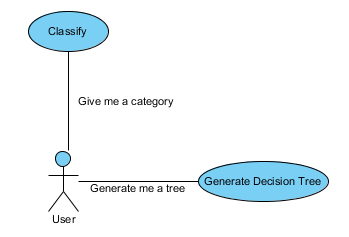
\includegraphics{UseCase_ID3.PNG}}
    \caption{Przypadek u�ycia dla algorytmu drzew decyzyjnych}
    \label{rys:useCaseID3}
    \end{center}
\end{figure}

Przeanalizujemy teraz diagram komponent�w~\ref{rys:componentDiagram}. Wyr�niamy nast�puj�ce elementy:
\begin{itemize}
\item \textbf{System} odpowiada aktorowi z diagramu~\ref{rys:useCaseID3}. Przewa�nie taki system operuje na zbiorze danych, kt�ry nie jest dopasowany do pracy z specyficznym formatem wymaganym przez algorytm. Dlatego pierwszym krokiem jaki wykonujemy, jest wykorzystanie komponentu \emph{Data Transformator} do transformacji danych (System Specific Data) tak, aby wygenerowane drzewo mog�o wykorzysta� ten zbi�r. Dodatkowo, programista odpowiedzialny za integracje mi�dzy \emph{Systemem}, a \emph{Data Transormatorem} musi dostarczy� plik mapowania danych, na podstawie kt�rego transformacja danych b�dzie wykonana. Dok�adne om�wienie tego mechanizmu znajdziemy w dalszej cz�ci rozdzia�u,
\item \textbf{Data Transformator} wspominany powy�ej komponent, s�u�y do przekszta�cania zbioru danych specyficznego dla \emph{Systemu} (System Specific Data) do postaci zgodnej z naszym algorytmem (Transformated Data),
\item \textbf{Data Loader} prosty komponent wczytuj�cy zbi�r danych w specyficznej dla naszego algorytmu postaci,
\item \textbf{Decision Tree Algorithm} rozszerzona implementacja algorytmu ID3~\ref{sec:algoytmyIndukcjiDrzewDecyzyjnychSchematOgolny} opisywana w tym rozdziale, wykorzystuje komponent \emph{Data Loader} do wczytania zbioru danych w celu wygenerowania drzewa decyzyjnego. Po wygenerowaniu drzewa, pozwala na klasyfikowanie obiekt�w zgodnych ze schematem dostarczonych danych.

\end{itemize}

\begin{figure}[ht]
    \begin{center}
    \fbox{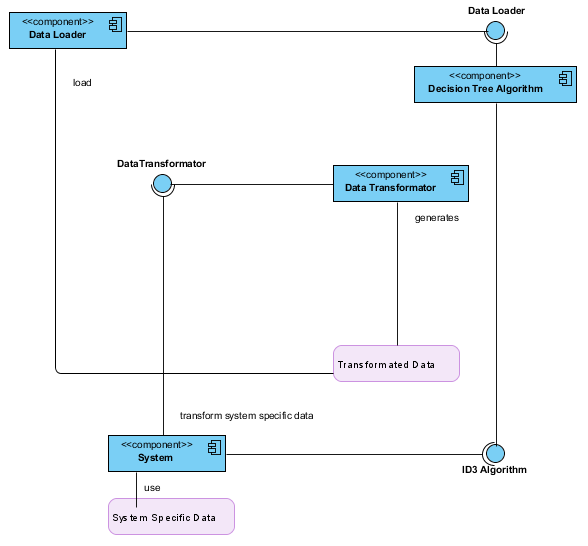
\includegraphics{ComponentDiagram.png}}
    \caption{Diagram komponent�w - przetwarzanie danych przez algorytm drzew decyzyjnych}
    \label{rys:componentDiagram}
    \end{center}
\end{figure}

Mamy teraz og�lny widok na struktur� algorytmu i komponent�w dodatkowych, wspieraj�cych warstw� przetwarzania danych. W dalszej cz�ci skupimy si� na om�wieniu dok�adnie poszczeg�lnych komponent�w, zaczynaj�c od cz�ci transformuj�cej dane specyficzne dla wykorzystuj�cego algorytm systemu.

%---------------------------------------------------------------------------
%---------------------------------------------------------------------------

\subsection{Data Transformator}
\label{sec:dataTransformator}
\begin{figure}[htb!]
    \begin{center}
    \fbox{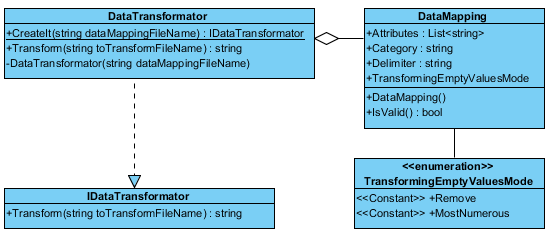
\includegraphics{DataTransformatorClassDiagram.png}}
    \caption{Diagram klas - komponent przetwarzaj�cy dane}
    \label{rys:dataTransformatorClass}
    \end{center}
\end{figure}

Komponent ten odpowiedzialny jest za transformacje danych, z formatu specyficznego dla klienta do formatu specyficznego dla naszego algorytmu drzew decyzyjnych. Jego struktura jest dosy� prosta, wida� j� na diagramie klas~\ref{rys:dataTransformatorClass}.

Komponent posiada jedn� metod� -- \emph{Transform}, kt�ra przyjmuje jako parametr nazw� pliku z danymi klienta, kt�re powinny by� przetworzone. Dodatkowo, podczas tworzenia komponentu za pomoc� metody \emph{CreateIt}, podajemy nazw� pliku mapowania danych. Struktura tego pliku zostanie om�wiona w dalszej cz�ci sekcji. Po utworzeniu komponentu jest tworzona instancja klasy, kt�ra przechowuje dane z pliku mapowania danych -- \emph{DataMapping}. Instancja ta mo�e by� stworzona tylko i wy��cznie podczas tworzenia komponentu \emph{Data Transformator} i jednocze�nie oznacza specjalizacj� komponentu transformacji dla konkretnego przypadku mapowania danych.

W czasie wykonywania metody \emph{Transform} mo�e zosta� rzucony wyj�tek typu \emph{DataTransformationException} gdy pojawi si� jakakolwiek b��d. Gdy wszystko zostanie wykonane poprawnie, w katalogu aplikacji wykorzystuj�cej komponent zostanie utworzony plik z przetworzonymi danymi. Nazwa tego pliku zostanie zwr�cona przez metod� \emph{Transform} po udanym zako�czeniu operacji.

\subsubsection*{Konfiguracja mapowania danych}

Sercem ca�ej operacji transformowania danych jest plik konfiguracyjny. Tak jak mo�na zobaczy� w przyk�adzie~\ref{ex:plikKonfiguracyjnyMapowanieDanych}, konfiguracja sk�ada si� z 4 w�a�ciwo�ci -- atrybuty (\emph{Attributes}), rodzaj operacji dla pustych danych (\emph{TransformingEmptyValuesMode}), kategoria (\emph{Category}) oraz ogranicznik (\emph{Delimiter}). Atrybuty, jak sama nazwa wskazuje, s� opisem poszczeg�lnych warto�ci obiektu dla okre�lonej domeny problemu. Kolejno�� atrybut�w okre�la kolejno�� warto�ci atrybut�w w pliku danych. Dodatkowo, w kategorii ustalamy, kt�ry z wymienionych atrybut�w jest atrybutem kategorii. Ma to znacz�cy wp�yw na wynikowy plik z danymi, poniewa� atrybut kategorii i wszystkie jego warto�ci jest przenoszony do ostatniej kolumny -- wzgl�dy optymalizacyjne. Pozosta�y nam dwa atrybuty. Ogranicznik definiuje, jakim znakiem (lub zbiorem znak�w) rozgraniczone s� kolejne warto�ci atrybut�w obiektu. Ostatni� w�asno�ci� jest wyb�r operacji dla pustych danych. Mamy dwie mo�liwo�ci - usuwanie niepe�nych danych lub przypisywanie wi�kszo�ciowej warto�ci atrybutu (kolejno - \emph{Remove, MostNumerous}).

\begin{sample}
\label{ex:plikKonfiguracyjnyMapowanieDanych}
Przyk�adowy plik konfiguracyjny dla danych z tabeli~\ref{tab:zbiorTrenujacyPogoda}:
\begin{lstlisting}[language=Xml]
<?xml version="1.0"?>
<DataMapping>
  <Attributes>
    <string>Aura</string>
    <string>Temperatura</string>
    <string>Wilgotno��</string>
    <string>Wiatr</string>
    <string>GramyWTenis</string>
  </Attributes>
  <TransformingEmptyValuesMode>
		Remove
  </TransformingEmptyValuesMode>
  <Category>GramyWTenis</Category>
  <Delimiter>;</Delimiter>
</DataMapping>
\end{lstlisting}
\end{sample}

Tak przygotowana konfiguracja przechodzi walidacj� podczas tworzenia komponentu s�u��cego do transformacji danych. Gdy wszystko idzie dobrze, dane z konfiguracji s� wykorzystywane do przetworzenia pliku danych specyficznych dla systemu i utworzenia finalnego pliku z danymi. Utworzone dane b�d� u�yte w procesie generowania drzewa, co zostanie om�wione w dalszej cz�ci rozdzia�u.

%---------------------------------------------------------------------------
%---------------------------------------------------------------------------

\subsection{Data Loader}

Komponent ten odpowiedzialny jest za wczytanie przygotowanego przez administratora systemu zbioru danych. Dodatkowo jego zadaniem jest przetworzenie zbioru danych z formatu specyficznego dla zewn�trznego systemu do postaci akceptowalnej przez omawiany komponent. Odbywa si� to za pomoc� komponentu transformacji danych opisywanego powy�ej~\ref{sec:dataTransformator}. 

Pocz�tkowo wykorzystuj�c �cie�k� do pliku z danymi komponent ten tworzy instancj� klasy~\emph{EntityData}. Instancja ta zawiera opis atrybut�w oraz zbi�r danych gotowy do dalszego przetworzenia. Pojedynczy obiekt jest definiowany jako obiekt klasy~\emph{DataRow}, czyli jako zbi�r warto�ci atrybut�w. Po wczytaniu z pliku danych, komponent~\emph{IDataLoader} wykorzystuje agregowan� instancj� klasy~\emph{IEntityDataValidator}, aby sprawdzi� poprawno�� wczytanych danych. Walidator zwraca obiekt klasy~\emph{Outcome}, kt�ry zawiera proste metody s�u��ce do sprawdzenia, czy operacja si� powiod�a. Dodatkowo mo�emy odczyta� wiadomo�� powi�zan� z b��dem, je�li taki wyst�pi�. Opisywane elementy mo�na zobaczy� na diagramie klas~\ref{rys:dataLoaderClass}.

\begin{figure}[ht]
    \begin{center}
    \fbox{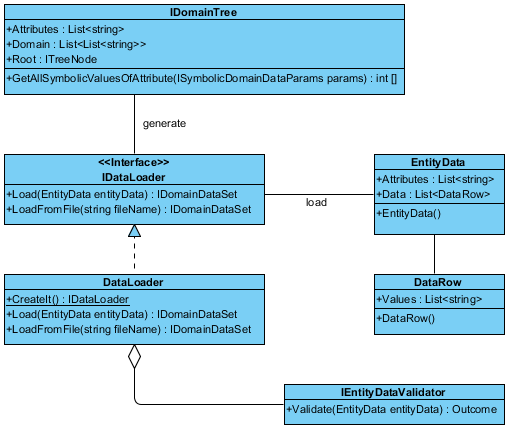
\includegraphics{DataLoaderClassDiagram.png}}
    \caption{Diagram klas - komponent wczytuj�cy dane}
    \label{rys:dataLoaderClass}
    \end{center}
\end{figure}

W tym momencie, kiedy nasz komponent ma opakowane dane, nast�puje ich przetwarzanie do instancji klasy implementuj�cej interfejs~\emph{IDomainTree}. Instancja ta b�dzie g��wn� struktur� danych (drzewem), na kt�rej b�dzie operowa� nasz algorytm drzew decyzyjnych i zostanie om�wiona dok�adnie w dalszej cz�ci. Kolejnymi etapami b�dzie generowanie drzewa oraz, w p�niejszym czasie, klasyfikacja obiekt�w.

%---------------------------------------------------------------------------
%---------------------------------------------------------------------------

\subsection{Domain Tree}

Pocz�tkowa posta� tej struktury jest tworzona przez wy�ej omawiany komponent -- \emph{DataLoader}. W pierwszej fazie struktura ta zawiera zbi�r atrybut�w oraz opis domeny. Opis domeny zawiera zbi�r mo�liwych warto�ci wszystkich atrybut�w, w postaci kolekcji warto�ci dla ka�dego atrybutu. Pozwala nam to na pewn� optymalizacje -- operacje por�wnywania w algorytmie drzew decyzyjnych b�d� wykonywany na liczbach ca�kowitych zamiast na zmiennych znakowych. Pomys� reprezentacji symbolicznej zosta� zaczerpni�ty z artyku�u dost�pnego w sieci~\cite{JavaIllustrations}. Dodatkowo do naszej dyspozycji pozostaje metoda~\emph{GetAllSymbolicValuesOfAttribute}. Metodzie tej podajemy symboliczne reprezentacje obiekt�w ze zbioru danych. W rezultacie pytamy j� o okre�lony symboliczny zbi�r wszystkich warto�ci znajduj�cych si� w podanym zbiorze danych dla konkretnego atrybutu, podaj�c jego indeks. Diagram klas dla omawianej struktury mo�na zobaczy� poni�ej~\ref{rys:dataTreeClass}.

\begin{figure}[ht]
    \begin{center}
    \fbox{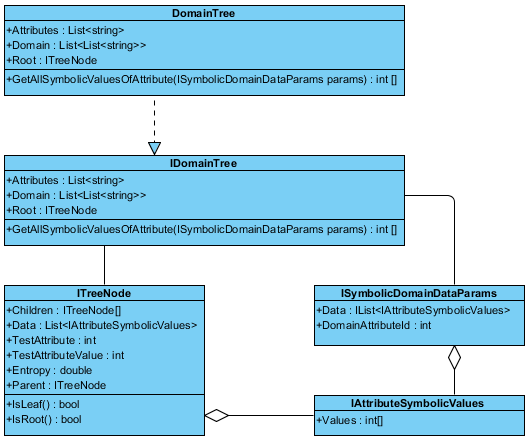
\includegraphics{DomainTreeClassDiagram.png}}
    \caption{Diagram klas - podstawowa struktura algorytmu}
    \label{rys:dataTreeClass}
    \end{center}
\end{figure}

W cz�ci omawiaj�cej dzia�anie algorytmu drzew decyzyjnych zostanie om�wiony proces generowania drzewa. Proces ten zaczyna si� od utworzenia korzenia, czyli instancji klasy implementuj�cej interfejs~\emph{ITreeNode} reprezentuj�cej korze� drzewa. Podczas pracy z struktur�~\emph{IDomainTree} b�dziemy operowa� na danych symbolicznych i wykorzystywa� implementacj� interfejsu~\emph{ISymbolicDomainDataParams}. Instancje tego interfejsu zawiera� b�d� pewien zbi�r przyk�ad�w reprezentowany w postaci symbolicznej oraz identyfikator atrybutu domeny. 

W tym momencie mamy przedstawione wszystkie potrzebne informacje, aby przej�� do om�wienia implementacji algorytmu drzew decyzyjnych. W naszym wypadku implementacja ta bazuje na podstawowym algorytmie ID3~\cite{Quin86}, w pewien spos�b go rozszerzaj�c.

%---------------------------------------------------------------------------
%---------------------------------------------------------------------------

\subsection{Decision Tree Algorithm}
\label{sec:decisionTreeAlgorithm}

Om�wienie algorytmu drzew decyzyjnych zaczniemy od opisu klasy pomocniczej~\emph{Entropy}. Klasa ta opakowuje nam obliczenia zwi�zane z wyznaczeniem entropii~\ref{eq:entropy}, zysku informacyjnego~\ref{eq:gainInformation} oraz ilorazu zysku informacyjnego~\ref{eq:gainRatio}, kt�re jak wiemy z rozwa�a� z rozdzia�u~\ref{cha:uczenieMaszynowe} s� nam niezb�dne. Diagram klasy~\emph{Entropy} znajduje si� na rysunku~\ref{rys:entropyClass}.

\begin{figure}[ht]
    \begin{center}
    \fbox{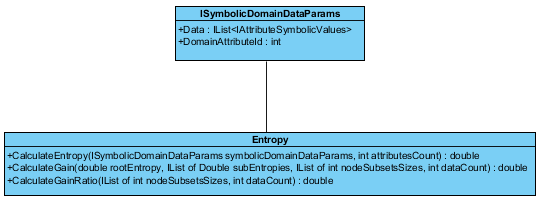
\includegraphics{EntropyClassDiagram.png}}
    \caption{Diagram klas - klasa opakowuj�ca obliczenia zwi�zane z wyznaczeniem entropii, zysku informacyjnego i ilorazu zysku informacyjnego}
    \label{rys:entropyClass}
    \end{center}
\end{figure}

Do dyspozycji mamy trzy metody:
\begin{itemize}
\item \textbf{CalculateEntropy} pozwala nam na wyliczenie entropii zgodnie ze wzorem~\ref{eq:entropy}, na podstawie zbioru przyk�ad�w w postaci symbolicznej oraz liczby atrybut�w.
\item \textbf{CalculateGain} pozwala nam na wyliczenie zysku informacyjnego zgodnie ze wzorem~\ref{eq:gainInformation}. Do wyznaczenia wyniku metoda u�ywa wyliczonych wcze�niej entropii dla poszczeg�lnych atrybut�w oraz entropii aktualnie analizowanego w�z�a.
\item \textbf{CalculateGainRatio} pozwala nam na wyliczenie ilorazu zysku informacyjnego zgodnie ze wzorem~\ref{eq:gainRatio}.
\end{itemize}

Mo�emy teraz przej�� do om�wienia w�asno�ci klasy~\emph{ID3Algorithm}, b�d�cej implementacj� interfejsu~\emph{IDecisionTreeAlgorithm}. Klasa ta implementuje rozszerzony algorytm ID3. Jej diagram klas znajduje si� na rysunku~\ref{rys:decisionTreeAlgorithmClass}. Jak widzimy na diagramie, algorytm wykorzystuje klas�~\emph{Entropy} do obliczania potrzebnych warto�ci. Dodatkowo, wykorzystuje struktury~\emph{IDomainTree} oraz~\emph{ITreeNode} do generowania drzewa i w p�niejszym czasie, do klasyfikowania przyk�ad�w. 

\begin{figure}[ht]
    \begin{center}
    \fbox{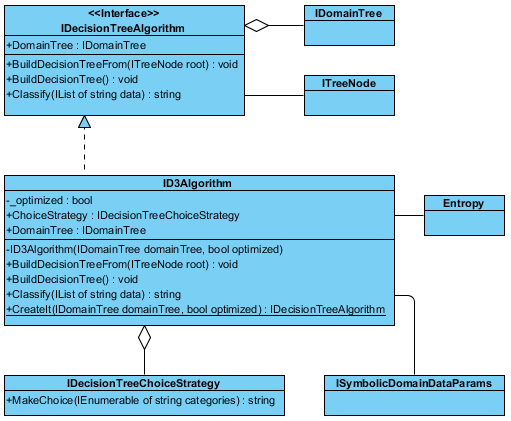
\includegraphics{DecisionTreeAlgorithmClassDiagram.png}}
    \caption{Diagram klas - algorytm tworzenia drzewa decyzyjnego i jego wykorzystania}
    \label{rys:decisionTreeAlgorithmClass}
    \end{center}
\end{figure}

Operacje budowania drzewa i klasyfikacji przyk�ad�w zostan� opisane dok�adnie poni�ej. Warto zwr�ci� uwag� na rozszerzenie zastosowane w algorytmie -- kompozycj� obiektu implementuj�cego interfejs~\emph{IDecisionTreeChoiceStrategy}. Element ten zosta� zaprojektowany, aby w przypadkach gdy podczas klasyfikacji zostanie wybranych kilka pasuj�cych kategorii, klient algorytmu m�g� dokona� w spos�b preferowany przez siebie wyboru poprzez podpi�cie swojej implementacji interfejsu~\emph{IDecisionTreeChoiceStrategy}. Domy�lna implementacja zwraca pierwsz� kategori� jako t� w�a�ciw�. Kolejn� rzecz�, o kt�rej warto wspomnie� jest mo�liwe uruchamianie algorytmu w dw�ch trybach. Zoptymalizowany tryb (flaga \emph{optimized} przy tworzeniu algorytmu ustawiona na \emph{true}) polega na wyznaczaniu wsp�czynnika trafno�ci wyboru atrybutu na podstawie zysku informacyjnego~\ref{eq:gainInformation}. Wersja niezoptymalizowana, b�d�ca jednocze�nie rozszerzon� wersj� algorytmu, bazuje na obliczeniu ilorazu zysku informacyjnego ze wzoru~\ref{eq:gainRatio}. Tryb ten jest w��czany poprzez ustawienie flagi~\emph{optimized} na warto��~\emph{false}. W cz�ci opisuj�cej przyk�ady poka�emy r�nice mi�dzy dzia�aniem obu tryb�w.

\subsubsection*{Budowanie drzewa}

\lstset{tabsize=2, basicstyle=\small}

\begin{lstlisting}[caption={Algorytm tworzenia drzewa decyzyjnego}, language=Java, frame = trBL, mathescape=true, label={lst:budujDrzewoID3}]
void budujDrzewo(ITreeNode korzen)
{
	idKategori = wyznaczIdKategorii();
	liczbaKategorii = wyznaczLiczbeKategorii();

	korzen.Entropy = Entropy.CalculateEntropy(...);

	if (entropiaRownaZero()) return;

	idNajlepszegoAtrybutu = wyznaczNajkorzystniejszyAtrybut(...);

	if (najlepszyAtrybutNieZostalWyznaczony()) return;

	liczbaWartosciNajlepszegoAtrybutu 
		= wyznaczLiczbeWartosciNajlepszegoAtrybutu(...);

	korzen.TestAttribute = idNajlepszegoAtrybutu;
	korzen.Children 
		= new TreeNode[liczbaWartosciNajlepszegoAtrybutu];

	for (id = 0; id < liczbaWartosciNajlepszegoAtrybutu; id++)
		przypiszNowyWezel(korzen, idNajlepszegoAtrybutu, id);

	foreach (var treeNode in korzen.Children)
		budujDrzewo(treeNode);
}
\end{lstlisting}

Powy�ej zosta� zamieszczony pseudokod operacji buduj drzewo~\ref{lst:budujDrzewoID3}. W zasadzie, wnikliwsza analiza nale�y si� dw�m metod�: metodzie \emph{wyznaczNajkorzystniejszyAtrybut(...)} oraz metodzie~\emph{przypiszNowyWezel(...)}. Sam algorytm bazuje na wcze�niej zamieszczonym algorytmie podstawowym~\ref{lst:budujDrzewo}. Metoda~\emph{przypiszNowyWezel(...)} tworzy now� instancj� klasy implementuj�cej interfejs~\emph{ITreeNode}, nast�pnie dodaje j� do dzieci aktualnie przetwarzanego w�z�a oraz przypisuje go jako rodzica oraz wyznacza podzbi�r danych dla testowanego atrybutu, kt�re s� z nim zgodne.

Operacja~\emph{wyznaczNajkorzystniejszyAtrybut(...)} wymaga wi�kszej uwagi. Poni�ej znajduje si� pseudokod operacji~\ref{lst:wyznaczNajlepszyAtrybut}. Jak mo�na zaobserwowa� w pseudokodzie, dla ka�dego atrybutu jest wyliczana warto�� entropii. Nast�pnie za pomoc� metody~\emph{CalculateGainFactor} wyliczany jest wska�nik zysku informacyjnego. W zale�no�ci od ustawienia wy�ej wspominanej w�asno�ci algorytmu~\emph{optimized}, je�li algorytm jest u�yty w wersji zoptymalizowanej, wyliczany jest ze wzoru~\ref{eq:gainInformation}, a w przeciwnym wypadku wyliczany jest iloraz ze wzoru~\ref{eq:gainRatio}. Je�li wsp�czynnik jest wy�szy od poprzednich, warto�� symboliczna atrybutu jest przechowywana jako najlepszy wyb�r testu dla aktualnie analizowanego w�z�a.

\lstset{tabsize=2, basicstyle=\small}

\begin{lstlisting}[caption={Operacja wyznaczenia najlepszego atrybutu do testu w w�le}, language=Java, frame = trBL, mathescape=true, label={lst:wyznaczNajlepszyAtrybut}]
int wyznaczLiczbeWartosciNajlepszegoAtrybutu(
	ITreeNode korzen, int liczbaKategorii, int idKategorii)
{
	for (idAtrybutu = 0; idAtrybutu < idKategorii; idAtrybutu++)
	{
		if (czyAtrybutBylJuzSprawdzany(idAtrybutu)) 
			continue;

		listaEntropii = stworzNowaListeEntropii();
		rozmiaryPodzbiorowElementowWezla = stworzNowaListe();

		liczbaWartosciAtrybutu = wyznaczLiczbeWartosci(idAtrybutu);

		for (wartoscSymboliczna = 0; 
			wartoscSymboliczna < liczbaWartosciAtrybutu; 
			wartoscSymboliczna++)
		{
			podzbiorElementow = 
				wezPodzbiorElementowPosiadajacychWartosc(wartoscSymboliczna);
			rozmiaryPodzbiorowElementowWezla.Add(podzbiorElementow.Count);

			if (podzbiorElementow.Count == 0) 
				continue;

			entropia = Entropy.CalculateEntropy(...);
			listaEntropii.Add(entropia);
		}

		wspolczynnikZyskuInformacyjnego = CalculateGainFactor(...);

		if (wspolczynnikZyskuInformacyjnego <= najlepszyWspolczynnik) 
			continue;

		najlepszyWspolczynnik = wspolczynnikZyskuInformacyjnego;
		najlepszyAtrybut = idAtrybutu;
	}

	return najlepszyAtrybut;
}
\end{lstlisting}

\subsubsection*{Klasyfikacja przyk�ad�w}

Klasyfikacja przyk�ad�w jest mo�liwa po wcze�niejszym wygenerowaniu drzewa decyzyjnego. Wystarczy wywo�a� operacj�~\emph{Classify} i jako argument poda� list� warto�ci atrybut�w obiektu w odpowiedniej kolejno�ci. Operacja ta przeszuka drzewo por�wnuj�c warto�ci atrybut�w i wyznaczy kilka lub jedn� dopasowan� kategori� (w naszej, podstawowej implementacji algorytm zawsze zwraca jedn� kategori�). Ostatecznie za pomoc� instancji klasy implementuj�cej interfejs~\emph{IDecisionTreeChoiceStrategy} wyliczane jest, kt�ra kategoria jest t� w�a�ciw�.

Na tym ko�czy si� przedstawienie warstwy przystosowania danych i implementacji algorytmu. W dalszej cz�ci poka�emy przyk�ady zastosowania poszczeg�lnych komponentu, a na ko�cu dokonamy podsumowania analizy przeprowadzonej w tym rozdziale.

%---------------------------------------------------------------------------

\section{Przyk�ady wykorzystania algorytmu i warstwy przystosowania danych}
\label{sec:przykladyWykorzystaniaAlgorytmuIWarstwyPrzystosowaniaDanych}

W rozdziale tym skupimy si� na przedstawieniu komponent�w omawianych powy�ej w dzia�aniu. Tak jak temat rozdzia�u sugeruje, nasze rozwa�ania podzielimy na dwie cz�ci: przyk�ady dla warstwy przystosowania danych oraz przyk�ady dla dzia�ania samego algorytmu.

%---------------------------------------------------------------------------
%---------------------------------------------------------------------------

\subsection{Warstwa przystosowania danych}

\subsubsection*{Data Transformator}

Pierwszym naszym przyk�adem b�dzie transformacja danych do postaci zgodnej z naszym algorytmem. Dane zamieszczone poni�ej~\ref{prz:daneDoTransofrmacji} zosta�y wzi�te z ksi��ki Toma Mitchella~\cite{Mit97}. Dotycz� one stanu pogody i podj�cia decyzji, czy gramy w tenisa czy nie. Dane sk�adaj� si� z pi�ciu atrybut�w: aura, temperatura, wilgotno��, wiatr i atrybut kategorii okre�laj�cy nasz� decyzj�, czy gramy w tenisa.

\begin{sample}
\label{prz:daneDoTransofrmacji}
Przyk�adowy zbi�r danych - dane opisuj�ce decyzj� czy gramy w tenisa, uzale�nion� od stanu pogody~\cite{Mit97}.

\begin{lstlisting}
No;sunny;Hot;High;Weak
No;sunny;Hot;High;Strong
Yes;Overcast;Hot;High;Weak
Yes;Rain;Mild;High;Weak
Yes;Rain;Cool;Normal;Weak
\end{lstlisting}
\end{sample}

Programista lub architekt odpowiedzialny za integracje systemu zewn�trznego z algorytmem tworzy plik mapowania danych. Dla przyk�adu danych~\ref{prz:daneDoTransofrmacji}, plik mapowania danych przedstawiony jest poni�ej~\ref{ex:plikKonfiguracjiDanychDlaPogoda}. W pliku tym definiujemy list� atrybut�w opisuj�ce nasze dane~\ref{prz:daneDoTransofrmacji}. Opisujemy jak nale�y post�powa� z niepe�nymi danymi (usuwanie przyk�ad�w), a nast�pnie okre�lamy kt�ry z atrybut�w jest atrybutem kategorii (PlayTennis). Na koniec, definiujemy ogranicznik danych (warto�ci atrybut�w), w tym przypadku b�dzie to �rednik.

\begin{sample}
\label{ex:plikKonfiguracjiDanychDlaPogoda}
Przyk�ad opisuje konfiguracje mapowania danych dla zbioru danych~\ref{prz:daneDoTransofrmacji}.

\begin{lstlisting}[language=Xml]
<?xml version="1.0"?>
<DataMapping>
  <Attributes>
    <string>PlayTennis</string>
    <string>Outlook</string>
    <string>Temperature</string>
    <string>Humidity</string>
    <string>Wind</string>
  </Attributes>
  <TransformingEmptyValuesMode>Remove</TransformingEmptyValuesMode>
  <Category>PlayTennis</Category>
  <Delimiter>;</Delimiter>
</DataMapping>
\end{lstlisting}
\end{sample}

Dla tak przygotowanych danych mo�emy u�y� programu~\emph{Agh.DecisionTree.DataTransformator.exe} przygotowanego wraz z prac�. Program ten wykorzystuje wcze�niej omawiany komponent transformacji danych~\ref{sec:dataTransformator}. Wywo�ujemy go z konsoli systemowej podaj�c mu dwa argumenty: �cie�k� pliku z danymi do transformacji oraz �cie�k� do pliku mapowania danych. W naszym wypadku, kiedy oba pliki~\ref{ex:plikKonfiguracjiDanychDlaPogoda} oraz \ref{prz:daneDoTransofrmacji} znajduj� si� w tym samym katalogu, wywo�anie wygl�da nast�puj�co: \emph{Agh.DecisionTree.DataTransformatorAgh.DecisionTree.DataTransformator.exe data.txt dataMapping.xml}. W wyniku wywo�ania programu otrzymujemy nast�puj�cy wynik:

\begin{sample}
\label{ex:danePrzetworzone}
Przetworzone dane~\ref{prz:daneDoTransofrmacji} z u�yciem konfiguracji mapowania danych~\ref{ex:plikKonfiguracjiDanychDlaPogoda}.

\begin{lstlisting}[language=Xml]
<?xml version="1.0"?>
<EntityData>
  <Attributes>
    <string>Wind</string>
    <string>Outlook</string>
    <string>Temperature</string>
    <string>Humidity</string>
    <string>PlayTennis</string>
  </Attributes>
  <Data>
    <DataRow>
      <Values>
        <string>Weak</string>
        <string>sunny</string>
        <string>Hot</string>
        <string>High</string>
        <string>No</string>
      </Values>
    </DataRow>
    <DataRow>
      <Values>
        <string>Strong</string>
        <string>sunny</string>
        <string>Hot</string>
        <string>High</string>
        <string>No</string>
      </Values>
    </DataRow>
    <DataRow>
      <Values>
        <string>Weak</string>
        <string>Overcast</string>
        <string>Hot</string>
        <string>High</string>
        <string>Yes</string>
      </Values>
    </DataRow>
    <DataRow>
      <Values>
        <string>Weak</string>
        <string>Rain</string>
        <string>Mild</string>
        <string>High</string>
        <string>Yes</string>
      </Values>
    </DataRow>
    <DataRow>
      <Values>
        <string>Weak</string>
        <string>Rain</string>
        <string>Cool</string>
        <string>Normal</string>
        <string>Yes</string>
      </Values>
    </DataRow>    
  </Data>
</EntityData>
\end{lstlisting}
\end{sample}

W pliku wynikowym~\ref{ex:danePrzetworzone} widzimy, �e zamieszczone zosta�y atrybuty w zmienionej kolejno�ci w taki spos�b, aby atrybut kategorii znalaz� si� na ostatnim miejscu. R�wnie� dla ka�dego przyk�adu warto�ci atrybut�w znalaz�y si� w odpowiedniej kolejno�ci. Wygenerowany plik jest kompletnym i wystarczaj�cym opisem zestawu danych, kt�ry w �atwy spos�b mo�na wczyta� do instancji klasy~\emph{EntityData}, u�ywanej podczas �adowania danych i tworzenia instancji klasy implementuj�cej interfejs~\emph{IDomainTree}.

Uwa�ny czytelnik zauwa�y, �e spos�b ten ma pewne ograniczenia. Jeste�my zmuszeni do przechowywania ca�ego zbioru danych w pami�ci, co mo�e by� dla bardzo du�ych zbior�w danych nie do przyj�cia. Dlatego wynik transformacji mo�e by� przechowywany w bazie danych i odpowiednio doczytywany w razie potrzeby. Jest to pierwsze mo�liwe rozszerzenie dla rozwi�zania opracowywanego w pracy.

\subsubsection*{Data Loader}

Dzia�anie tego komponentu jest prostsze ni� pozosta�ych, dlatego om�wimy og�lnie jego zadanie bez szczeg�owego przyk�adu. Zadaniem komponentu jest przede wszystkim wczytanie pliku utworzonego przez komponent transformuj�cy dane~\ref{sec:dataTransformator}, a nast�pnie walidacja poprawno�ci utworzonej struktury z danymi.

Po udanej weryfikacji wczytywanego pliku, tworzona jest struktura drzewa (\emph{IDomainTree}), kt�ra b�dzie wykorzystywana przy generowaniu drzewa decyzyjnego. Przepisywana jest kolekcja atrybut�w, a nast�pnie definiowana jest domena problemu poprzez zdefiniowanie kolekcji atrybut�w. Do ka�dego atrybutu przypisujemy kolekcje mo�liwych warto�ci, a indeksy poszczeg�lnych warto�ci stanowi� b�d� symboliczn� reprezentacje przyk�ad�w domeny. Przyk�ady w symbolicznej postaci zapisywane s� jako dane, w nowo utworzonym drzewie.

%---------------------------------------------------------------------------
%---------------------------------------------------------------------------

\subsection{Algorytm drzew decyzyjnych}

Na sam koniec, przedstawimy przyk�ady dzia�ania naszego algorytmu. Algorytm w tej cz�ci pracy b�dzie uczony ma�ymi zbiorami danych przyk�ad�w, o niewielkiej liczbie atrybut�w tak, aby pokaza� jego przyk�adowe dzia�anie. Bardziej �yciowe przyk�ady zostan� przedstawione w rozdziale~\ref{cha:wynikiBadanEksperymentalnych}.

Aby pokaza� jak dzia�a, wykorzystamy ma�y zbi�r danych zaczerpni�ty ze strony internetowej~\cite{JavaIllustrations}. Przyk�ad~\ref{ex:bridgeData} reprezentuje dane powi�zane z in�ynieri� budowy most�w.

\begin{sample}
\label{ex:bridgeData}
Plik bridges.dat

\begin{lstlisting}
Span		Shape		Slab
//**************************************
long		square		waffle
long		rectangle	waffle
short		square		two-way
short		rectangle	one-way
\end{lstlisting}
\end{sample}

Dla naszych danych wywo�ujemy program: \emph{Agh.DecisionTree.ID3.Program.exe bridges.dat}. W wyniku otrzymujemy nast�puj�ce drzewo:

\begin{figure}[ht]
    \begin{center}
    \fbox{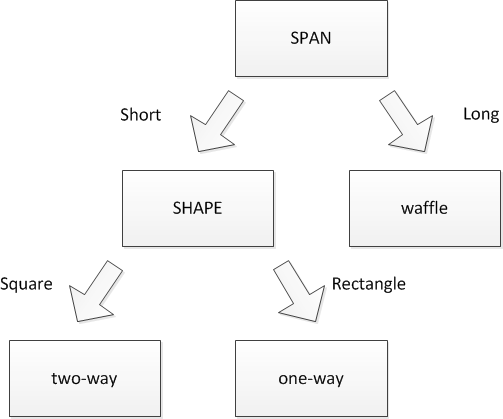
\includegraphics{bridgeTree.png}}
    \caption{Drzewo decyzyjne utworzone za pomoc� naszego algorytmu dla pliku bridges.dat~\ref{ex:bridgeData}}
    \label{rys:bridgeTree}
    \end{center}
\end{figure}

Na rysunku~\ref{rys:bridgeTree} wida� wyra�nie, �e najwi�kszy zysk informacyjny jest dla atrybutu \emph{span}, kt�ry pozwala nam od razu wybra� klas� \emph{waffle} gdy warto�� atrybutu wynosi~\emph{Long}. Drugim w kolejno�ci atrybutem jest atrybut~\emph{shape}, kt�ry dzieli nasze egzemplarze na dwie kategorie:~\emph{two-way} oraz~\emph{one-way}.

Poni�ej zosta� zamieszczony fragment kodu w j�zyku C\#~\ref{ex:kodBridgeTree}, kt�ry wykorzystuje bibliotek� stworzon� dla cel�w pracy magisterskiej. Pocz�tkowo deklarujemy referencje do implementacji algorytmu, a nast�pnie tworzymy komponent do �adowania danych, wstrzykuj�c mu domy�lny walidator danych. Kolejno, �adujemy dane z pliku~\emph{bridges.xml}, kt�ry to zosta� utworzony przez komponent transformacji danych dla pliku~\ref{ex:bridgeData}. W tym momencie mo�emy wykorzysta� utworzon� struktur�~\emph{domainTree} do wygenerowania drzewa decyzyjnego. W tym celu wykorzystujemy metod�~\emph{CreateIt} do wstrzykni�cia wspomnianej struktury danych i wywo�ujemy metod�~\emph{BuildDecisionTree}. Wygenerowane drzewo pos�u�y nam do klasyfikacji przyk�adu, kt�rego warto�ci atrybut�w~\emph{Span}~i~\emph{Shape} to odpowiednio:~\emph{short} oraz~\emph{rectangle}. W wyniku wywo�ania metody~\emph{Classify} otrzymujemy dopasowan� kategori� do testowanego obiektu, w tym przypadku jest to klasa~\emph{one-way}. Odpowiada to wy�ej zamieszczonemu drzewu decyzyjnemu na rysunku~\ref{rys:bridgeTree}.

\begin{lstlisting}[caption={Przyk�adowy kod w j�zyku C\# wykorzystuj�cy drzewo decyzyjne}, language=Java, frame = trBL, mathescape=true, label={ex:kodBridgeTree}]
ID3Algorithm _id3;

IDataLoader loader = 
	DataLoader.CreateIt(EntityDataValidator.CreateIt());

var domainTree = loader.LoadFromFile("bridges.xml");

_id3 = ID3.ID3Algorithm.CreateIt(domainTree);
_id3.BuildDecisionTree();

// short;rectangle;one-way

var data = new List<string> { "short", "rectangle" };

string classification = _id3.Classify(data);

Assert.That(classification, Is.EqualTo("one-way"));

\end{lstlisting}

Innym ciekawym przyk�adem generowania drzewa decyzyjnego jest wygenerowane drzewo na podstawie pliku z danymi~\ref{ex:strategieMarketingowe}, w zale�no�ci od zastosowanego parametru~\emph{optimized}~\ref{sec:decisionTreeAlgorithm}. Odrazu wida�, �e plik z danymi jest obszerniejszy od wcze�niej analizowanego~\ref{ex:bridgeData}. W tym przyk�adzie ujawnia si� niechciana cecha podstawowej wersji algorytmu ID3, o kt�rej wspominali�my w rozdziale~\ref{sec:realizacjaSchematuOgolnegoKryteriumStopu}. 

\lstset{tabsize=2, basicstyle=\small}

\begin{sample}
\label{ex:strategieMarketingowe}
Zestaw danych opisuj�cy fikcyjne strategie marketingowe~\cite{DecisionTreesNet}.

\begin{lstlisting}
Date			District	House_Type		Income	Prev. Customer Outcome
//*******************************************************************
3/10/03		Suburban	Detached			High		No						Nothing
14/9/03		Suburban	Detached			High		Responded			Nothing
2/4/02		Rural			Detached			High		No						Responded
18/1/03		Urban			Semi-detached	High		No						Responded
3/4/03		Urban			Semi-detached	Low			No						Responded
15/10/02	Urban			Semi-detached	Low			Responded			Nothing
15/10/02	Rural			Semi-detached	Low			Responded			Responded
2/3/01		Suburban	Terrace				High		No						Nothing
4/5/03		Suburban	Semi-detached	Low			No						Responded
2/1/03		Urban			Terrace			Low			No						Responded
3/10/03		Suburban	Terrace			Low			Responded			Responded
3/10/03		Rural			Terrace			High		Responded			Responded
8/4/03		Rural			Detached		Low			No						Responded
6/5/02		Urban			Terrace			High		Responded			Nothing
\end{lstlisting}
\end{sample}

W tym przypadku, wynikowe drzewa (ze wzgl�du na ich obj�to��) przedstawimy za pomoc� regu�. Regu�y b�d� zbiorem kolejnych wyra�e� warunkowych. Poni�sze drzewo~\ref{ex:drzewoZoptymalizowane} zosta�o wygenerowane za pomoc� algorytmu wykorzystuj�cego tylko obliczenia na podstawie~\emph{zysku informacyjnego}, przez co drzewo w stosunku do drzewa nieoptymalizowanego jest d�u�sze, jednak czas potrzebny na wygenerowanie drzewa jest stosunkowo kr�tszy.

\lstset{tabsize=2, basicstyle=\small}

\begin{sample}
\label{ex:drzewoZoptymalizowane}
Wygenerowane drzewo z parametrem~\emph{optimized} o warto�ci~\emph{true}.

\begin{lstlisting}[language=Java, frame = trBL]
if ( Date == "3/10/03") {
	if( Previous_Customer == "No") {
		Outcome = "Nothing";
	} else  if( Previous_Customer == "Responded") {
		Outcome = "Responded";
	}
} else if( Date == "14/9/03") {
	Outcome = "Nothing";
} else if( Date == "2/4/02") {
	Outcome = "Responded";
} else if( Date == "18/1/03") {
	Outcome = "Responded";
} else if( Date == "3/4/03") {
	Outcome = "Responded";
} else if( Date == "15/10/02") {
	if( Previous_Customer == "No") {
		Outcome = undefined;
	} else  if( Previous_Customer == "Responded") {
		if( Income == "High") {
			Outcome = undefined;
		} else if( Income == "Low") {
			if( House_Type == "Detached") {
				Outcome = undefined;
			} else if( House_Type == "Semi-detached") {
				if( District == "Suburban") {
					Outcome = undefined;
				} else if( District == "Rural") {
					Outcome = "Responded";
				} else if( District == "Urban") {
					Outcome = "Nothing";
				}
			} else if( House_Type == "Terrace") {
				Outcome = undefined;
			}
		}
	}
} else if( Date == "2/3/01") {
	Outcome = "Nothing";
} else if( Date == "4/5/03") {
	Outcome = "Responded";
} else if( Date == "2/1/03") {
	Outcome = "Responded";
} else if( Date == "8/4/03") {
	Outcome = "Responded";
} else if( Date == "6/5/02") {
	Outcome = "Nothing";
}
\end{lstlisting}
\end{sample}

Drzewo wygenerowane z wykorzystaniem~\emph{ilorazu zysku informacyjnego} jest p�ytsze i mniejsze, przez co pozwala na lepsze dopasowywanie przyk�ad�w, zw�aszcza tych nie pokrywaj�cych si� bezpo�rednio z przyk�adami ze zbioru testowego. Widzimy r�wnie�, �e promowany przez powy�sze drzewo~\ref{ex:drzewoZoptymalizowane} atrybut~\emph{Prev. Customer} ze wzgl�du na liczno�� wyst�powania warto�ci atrybutu, nie jest ju� preferowanym atrybutem w drzewie~\ref{ex:drzewoNieoptymalizowane}. Pozwoli�o to na uzyskanie lepszego drzewa, kosztem czasu generowania drzewa decyzyjnego.

\lstset{tabsize=2, basicstyle=\small}

\begin{sample}
\label{ex:drzewoNieoptymalizowane}
Wygenerowane drzewo z parametrem~\emph{optimized} o warto�ci~\emph{false}.

\begin{lstlisting}[language=Java, frame = trBL]
if( Date == "3/10/03") {
	if( House_Type == "Detached") {
		Outcome = "Nothing";
	} else  if( House_Type == "Semi-detached") {
		Outcome = undefined;
	} else  if( House_Type == "Terrace") {
		Outcome = "Responded";
	}
} else if( Date == "14/9/03") {
	Outcome = "Nothing";
} else if( Date == "2/4/02") {
	Outcome = "Responded";
} else if( Date == "18/1/03") {
	Outcome = "Responded";
} else if( Date == "3/4/03") {
	Outcome = "Responded";
} else if( Date == "15/10/02") {
	if( District == "Suburban") {
		Outcome = undefined;
	} else  if( District == "Rural") {
		Outcome = "Responded";
	} else  if( District == "Urban") {
		Outcome = "Nothing";
	}
} else if( Date == "2/3/01") {
	Outcome = "Nothing";
} else if( Date == "4/5/03") {
	Outcome = "Responded";
} else if( Date == "2/1/03") {
	Outcome = "Responded";
} else if( Date == "8/4/03") {
	Outcome = "Responded";
} else if( Date == "6/5/02") {
	Outcome = "Nothing";
}
\end{lstlisting}
\end{sample}

%---------------------------------------------------------------------------

\section{Podsumowanie}
\label{sec:implementacjaAlgorytmuPodsumowanie}

Aktualnie mamy �wiadomo��, jak wygl�da implementacja algorytmu przedstawionego w teoretycznym rozdziale~\ref{cha:uczenieMaszynowe}. Wiemy z jakich komponent�w sk�ada si� ca�o��, pozwalaj�ca nie tylko na wygenerowanie drzewa decyzyjnego i klasyfikacje przyk�ad�w, ale r�wnie� warstwa przetwarzania danych. W�a�ciwie to od tej warstwy zale�y praktyczna u�yteczno�� implementacji konkretnego algorytmu. Gdy jeste�my w stanie dowolne specyficzne dane wykorzysta� w istniej�cym algorytmie, w�wczas mo�emy czerpa� wszelakie korzy�ci id�ce z zastosowanym algorytmem.

Wprowadzone rozszerzenie algorytmu, pozwalaj�ce na definiowanie strategii, gdy algorytm zwr�ci nam wiele odpowiadaj�cych kategorii, w doskona�y spos�b wpasowuje si� w problem rozwa�any w pracy. Za��my, �e zadanie zosta�o dopasowane do kilku pracownik�w. Najprostszym kryterium wyboru tak ograniczonego zbioru ze wszystkich pracownik�w mo�e by� ich obci��enie. Zatem bezpo�rednio jeste�my w stanie poprzez to rozszerzenie wp�ywa� na dane wynikowe, co r�wnie� ma ogromne znaczenie na u�yteczno�� algorytmu uczenia maszynowego.

W nast�pnym rozdziale zostanie przedstawiona platforma do zarz�dzania zadaniami stworzona na cele pracy. Dopiero kolejny rozdzia�, czyli po��czenie implementacji algorytmu oraz stworzonej platformy poka�e nam prawdziw� si�� algorytm�w uczenia maszynowego. Na przypadkach zbli�onych do realnych problem�w prze�ledzimy zalety wykorzystania metod uczenia maszynowego. Dodatkowo zwr�cimy uwag� na problemy powi�zane z integracj� takiego algorytmu z istniej�cym systemem.



















\chapter{System zarz�dzania zadaniami}
\label{cha:systemZarzadzaniaZadaniami}

W czwartym rozdziale skupimy si� na przedstawieniu platformy s�u��cej do zarz�dzania zadaniami na przyk�adzie firmy informatycznej. Opiszemy system i jego funkcje, wraz z podzia�em na role. Na koniec opisane zostan� dane przygotowane dla cel�w pracy, kt�re zostan� wykorzystane w badaniach i analizach w rozdziale~\ref{cha:wynikiBadanEksperymentalnych}. 
Rozdzia�~\ref{cha:wynikiBadanEksperymentalnych} wykorzystuje po��czenie systemu zarz�dzania zadaniami i algorytmu drzew decyzyjnych. Po��czenie to jest przedstawione pod koniec tego rozdzia�u.

%---------------------------------------------------------------------------

\section{Opis systemu}
\label{sec:opisSystemu}

System zarz�dzania zadaniami, jak sama nazwa wskazuje, ma na celu umo�liwi� definiowanie zada�, ich zarz�dzanie poprzez przypisywanie do konkretnych os�b i raportowanie czasu, stanu realizacji zada� przez osoby wykonuj�ce. Te dwa zadania s� przypisane kolejno do roli menad�era oraz do roli pracownika (w tym przypadku, programisty). Dodatkowo w systemie znajduje si� rola administratora, kt�ry pozwala na definiowanie nowych pracownik�w i innych rzeczy administracyjnych potrzebnych do pracy dw�m wcze�niej wymienionym rol�.

System zosta� napisany przy u�yciu j�zyka C\#\cite{CSharpWiki}. Jako technologi� pozwalaj�c� utworzy� platform� internetow� zosta�a u�yta technologia ASP.NET MVC 3~\cite{AspNetMvc}. Do integracji z baz� danych wykorzystali�my Entity Framemework 4~\cite{EntityFramework}, a sama baza zosta�a utworzona przy pomocy serwera MS SQL Server 2008~\cite{SqlServer}. W dalszej cz�ci nie b�dziemy si� odwo�ywa� do specyficznych technologicznych niuans�w powi�zanych z wy�ej wymienionymi technologiami. Po bardziej szczeg�owe informacje nale�y uda� si� do wymienionych odno�nik�w.

%---------------------------------------------------------------------------
%---------------------------------------------------------------------------
\subsection{Model danych}

W cz�ci tej skupimy si� na opisie modelu danych. Obrazowo model ten przedstawiony jest na poni�szym diagramie~\ref{rys:dbDiagram} tabel bazy danych u�ywanej podczas pracy z systemem zarz�dzania zadaniami.

\begin{figure}[ht]
    \begin{center}
    \fbox{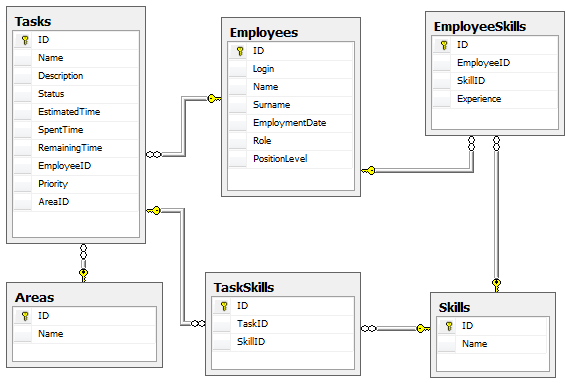
\includegraphics{DbDiagram.PNG}}
    \caption{Diagram tabel dla bazy danych systemu zarz�dzania zadaniami}
    \label{rys:dbDiagram}
    \end{center}
\end{figure}

Model danych jest podzielony na 4 elementy, przy czym na diagramie mo�na zaobserwowa� a� 6 tabel. Wynika to z prostego faktu, tzn. dwie dodatkowe tabele s� tabelami ��cznikowymi wiele do wiele pozwalaj�ce uzyska� nam oczekiwane powi�zanie mi�dzy konkretnymi typami danych. Dodatkowo tabela ��cz�ca pracownika z umiej�tno�ci� (\emph{EmployeeSkills}) posiada dodatkowy parametr, okre�laj�cy stopie� zaawansowania danej umiej�tno�ci (\emph{Experience}). Poni�ej zosta�y opisane cztery podstawowe elementy modelu danych:
\begin{itemize}
\item \textbf{Tasks} jest tabel� odpowiedzialn� za przechowywanie zada�. Ka�de zadanie opr�cz opisowych danych takich jak nazwa, opis, posiada przypisanego pracownika, kt�ry praktycznie rzecz bior�c b�dzie klas�, do kt�rej b�dziemy chcieli przypisa� dane zadanie. Dodatkowo, do zadania przypisujemy obszar funkcjonalny (\emph{Area}). Pozosta�e parametry s� powi�zane z statusem i priorytetem zadania oraz z raportowanym i estymowanym czasem zadania. Dodatkowo, zadania opisywane s� za pomoc� tabeli ��cznikowej~\emph{TaskSkills}, kt�ra okre�la wymagane lub wskazane umiej�tno�ci potrzebne do realizacji danego zadania.
\item \textbf{Employees} jest tabel� przechowuj�ca pracownik�w przypisanych do roli menad�era lub programisty. Typ pracownika jest okre�lony za pomoc� parametru~\emph{Role}. Dodatkowo, tabela zawiera dane opisowe pracownika takie jak jego login, imi� i nazwisko, data zatrudnienia oraz pozycja stanowiska. Dodatkowym opisem pracownik�w jest tabela ��cznikowa~\emph{EmployeeSkills} zwieraj�ca przypisane umiej�tno�ci i ich poziom do pracownika.
\item \textbf{Areas} to prosta tabela zawieraj�ca nazw� obszaru funkcjonalnego, kt�ry jest cz�ci� ca�ej domeny interesuj�cej dan� firm�. 
\item \textbf{Skills} to kolejna prosta tabela zawieraj�ca nazw� umiej�tno�ci powi�zanej w pewien spos�b z programowaniem (nasz konkretny przyk�ad zarz�dzania zadaniami).

\end{itemize}

%---------------------------------------------------------------------------
%---------------------------------------------------------------------------
\subsection{Architektura systemu}

Architektura systemu jest stosunkowo prosta. Mamy trzy warstwy, warstw� prezentacji w postaci aplikacji internetowej, do kt�rej u�ytkownik musi si� zalogowa�. Ciekawym faktem jest, �e warstwa ta ca�kowicie r�ni si� w zale�no�ci od roli pracownika. Menad�er ma do dyspozycji ca�kiem inne ekrany, ni� te pozostaj�ce do dyspozycji programisty czy administratora. Dodatkowym narz�dziem warstwy prezentacji u�ywanym przez administratora, jest aplikacja internetowa do zarz�dzania rolami na bazie danych stworzona przez firm� Microsoft.

Warstwa biznesowa jest odpowiedzialna za przechwytywanie zdarze� warstwy prezentacji i odpowiednie przetwarzanie danych. Do jej stworzenia zosta�y u�yte wcze�niej wspominane technologie, ASP.NET MVC jako cz�� pozwalaj�ca na utworzenie i integracj� warstwy prezentacji i warstwy biznesowej oraz Entity Framework jako framework pozwalaj�cy wsp�pracowa� z baz� danych.

Ostatni� warstw� jest warstwa danych, kt�ra ogranicza si� do bazy danych utworzonej za pomoc� serwera MS Sql Server 2008. Model bazy zosta� zaprezentowany powy�ej na diagramie~\ref{rys:dbDiagram}.

%---------------------------------------------------------------------------
%---------------------------------------------------------------------------
\subsection{Role w systemie zarz�dzania zadaniami}

Tak jak wy�ej wspomnieli�my, w systemie mamy wyr�nione trzy role: menad�er, programista (in�ynier) oraz administrator. Administrator skupia si� na zarz�dzaniu ca�� infrastruktur� systemu, natomiast funkcjonalno�� biznesowa systemu jest wykorzystywana przez menad�era i programist�.

\subsubsection*{Administrator}

Poni�ej zamieszczony jest diagram przypadk�w u�ycia opisuj�cy zadania wykonywane przez administratora~\ref{rys:administratorUseCase}.

\begin{figure}[ht]
    \begin{center}
    \fbox{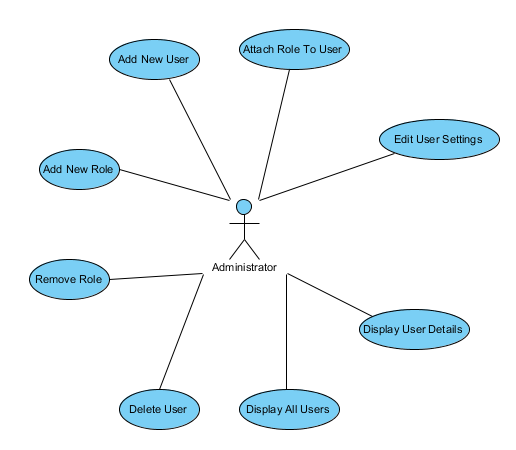
\includegraphics{AdministratorUseCase.png}}
    \caption{Diagram przypadk�w u�ycia dla roli Administrator}
    \label{rys:administratorUseCase}
    \end{center}
\end{figure}

Trzy przypadki u�ycia s� wykonywane przez administratora za pomoc� narz�dzia~\emph{ASP.NET Web Site Administration Tool}. Opis narz�dzia wraz z odniesieniami do szczeg�owych informacji mo�na znale�� na stronie~\cite{AspNetAdministrationTool}. Wspomniane przypadki to \emph{Add New Role}, \emph{Remove Role} oraz \emph{Atach Role To User}, czyli innymi s�owy m�wi�c zarz�dzanie rolami wyst�puj�cymi w aplikacji. Jako �e aplikacja ma trzy predefiniowane role i zakres pracy nie przewiduje rozszerzania liczby r�l, interesuj�cym przypadkiem b�dzie dla nas jedynie przypisywanie roli do u�ytkownika. Dodatkowo, dwa przypadki u�ycia s�u��ce do dodawania i usuwania u�ytkownik�w aplikacji (\emph{Add New User}, \emph{Delete User}) s� realizowane po cz�ci po stronie wymienionego narz�dzia, a po cz�ci po stronie systemu do zarz�dzania zadaniami. Dok�adniejszy opis tych przypadk�w u�ycia znajduje si� poni�ej.

Przypadki u�ycia dla roli administratora:
\begin{itemize}
\item \textbf{Add New Role} to jedynie dodanie litera�u definiuj�cego rol� u�ytkownika. Role te s� wykorzystywane w aplikacji do ograniczania uprawnie� (lub ich nadawania) dla poszczeg�lnych u�ytkownik�w systemu w zale�no�ci od przypisanych do nich r�l. W aplikacji mamy predefiniowane trzy role: menad�er, administrator oraz programista (in�ynier). W czasie pracy nie b�dziemy zmienia� liczby r�l.
\item \textbf{Remove Role} pozwala na usuni�cie wcze�niej dodanej roli do systemu.
\item \textbf{Attach Role To User} przypisuje wybran� rol� do u�ytkownika. U�ytkownik po stworzeniu i dodaniu do systemu nie ma dost�pu do �adnych interesuj�cych funkcjonalno�ci systemu. Dopiero po przypisaniu mu roli, funkcjonalno�ci powi�zane z dan� rol� w systemie s� dla niego dost�pne.
\item \textbf{Add New User} polega na dodaniu nowego u�ytkownika do systemu. Jest to proces dwu stopniowy. Pierwszy polega na dodaniu u�ytkownika za pomoc� narz�dzia ASP.NET Web Site Administration Tool do bazy danych. Podajemy w�wczas jedynie login u�ytkownika, mail oraz has�o. Reszta danych b�dzie tworzona w drugiej fazie, kt�r� wykonujemy w systemie zarz�dzania zadaniami. Aby u�ytkownik w pe�ni m�g� korzysta� z systemu, administrator musi zalogowa� si� do naszego systemu i tam wybra� spo�r�d nowo dodanych u�ytkownik�w w pierwszej fazie interesuj�cej go osoby, a nast�pnie przypisa� do niej pozosta�e dane. Tak utworzony u�ytkownik jest pe�noprawnym u�ytkownikiem systemu zarz�dzania zadaniami.
\item \textbf{Delete User} pozwala na usuni�cie istniej�cego u�ytkownika. R�wnie� jest to proces dwu stopniowy, lecz wykonujemy go w odwrotnej kolejno�ci w stosunku do powy�szego przypadku u�ycia.
\item \textbf{Display All Users} pozwala zalogowanemu do systemu administratorowi wy�wietli� informacje na temat wszystkich u�ytkownik�w systemu.
\item \textbf{Display User Details} polega na wy�wietleniu danych konkretnego u�ytkownika systemu.
\item \textbf{Edit User Settings} pozwala zalogowanemu do systemu administratorowi edytowa� dane u�ytkownika systemu.

\end{itemize}

\subsubsection*{Programista (in�ynier)}

Je�li chodzi natomiast o dwie pozosta�e role, wszystkie ich przypadki u�ycia realizowane s� w systemie zarz�dzania zadaniami.

Poni�ej zamieszczony jest diagram przypadk�w u�ycia opisuj�cy zadania wykonywane przez programist�~\ref{rys:engineerUseCase}.

\begin{figure}[ht]
    \begin{center}
    \fbox{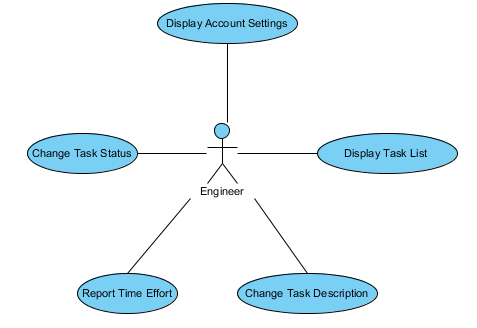
\includegraphics{EngineerUseCase.png}}
    \caption{Diagram przypadk�w u�ycia dla roli Engineer}
    \label{rys:engineerUseCase}
    \end{center}
\end{figure}

Przypadki u�ycia dla roli programisty to:
\begin{itemize}
\item \textbf{Display Account Settings} polega na wy�wietleniu przez u�ytkownika danych na jego temat.
\item \textbf{Display Task List} pozwala programi�cie przegl�da� list� przypisanych do niego zada�. Bezpo�rednio z tej listy mo�e przej�� do edycji konkretnego zadania w zale�no�ci od post�p�w pracy.
\item \textbf{Change Task Status} polega na zmianie statusu zadania w zale�no�ci od post�p�w pracy. Zadanie mo�e znajdowa� si� w czterech stanach: \emph{new} - zaraz po utworzeniu i przypisaniu do konkretnej osoby, \emph{open} - podczas pracy nad zadaniem, \emph{close} - po zako�czeniu zadania oraz \emph{cancel} gdy zadanie zosta�o anulowane.
\item \textbf{Report Time Effort} polega na aktualizowaniu czasu zwi�zanego z zadaniem. Do dyspozycji programisty s� trzy warto�ci: \emph{estimation} uzupe�niana na pocz�tku, stanowi�ca oszacowanie czasu potrzebnego na realizacj� zadania, \emph{completed} wskazuj�ca liczb� godzin sp�dzonych na realizacji zadania oraz \emph{remaining} stanowi�ca oszacowanie liczby godzin potrzebnych jeszcze do zako�czenia zadania.
\item \textbf{Change Task Description} pozwala programi�cie zmienia� opis zadania, np. poprzez dodanie komentarza opisuj�cego rozwi�zywane zadanie lub problemy, kt�re pojawi�y si� podczas realizacji zadania.

\end{itemize}

\subsubsection*{Menad�er}

Poni�ej zamieszczony jest diagram przypadk�w u�ycia opisuj�cy zadania wykonywane przez menad�era~\ref{rys:managerUseCase}.

\begin{figure}[ht]
    \begin{center}
    \fbox{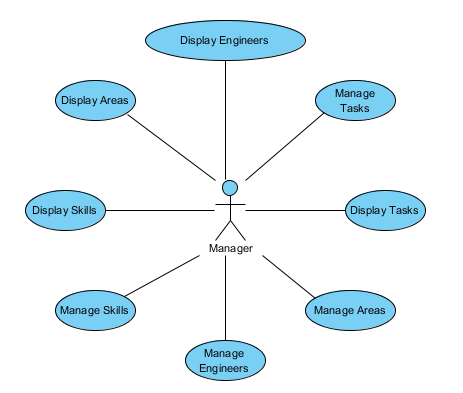
\includegraphics{ManagerUseCase.png}}
    \caption{Diagram przypadk�w u�ycia dla roli Manager}
    \label{rys:managerUseCase}
    \end{center}
\end{figure}

Przypadki u�ycia dla roli menad�era:
\begin{itemize}
\item \textbf{Display Skills} polega na wy�wietleniu dodanych do systemu umiej�tno�ci, kt�re mog� zosta� przypisane do programist�w.
\item \textbf{Manage Skills} polega na dodawaniu, usuwaniu i edycji umiej�tno�ci w systemie zarz�dzania zadaniami.
\item \textbf{Display Areas} polega na wy�wietleniu dodanych do systemu obszar�w funkcjonalno�ci, kt�re mog� zosta� przypisane do konkretnych zada�.
\item \textbf{Manage Areas} polega na dodawaniu, usuwaniu i edycji obszar�w funkcjonalnych w systemie zarz�dzania zadaniami.
\item \textbf{Display Tasks} polega na wy�wietleniu dodanych do systemu zada�, kt�re nie zosta�y jeszcze przypisane do �adnego programisty (s� przypisane do menad�era).
\item \textbf{Manage Tasks} polega na dodawaniu, usuwaniu i edycji zada�, kt�re powinny by� wykonane przez programist�w. Dodatkowo przypadek u�ycia zawiera w sobie mo�liwo�� przypisania zadania do konkretnego programisty, co skutkuje tym, �e zadanie nie jest ju� wy�wietlane na tablicy zada� menad�era oraz menad�er nie mo�e ju� zarz�dza� danym zadaniem.
\item \textbf{Display Engineers} polega na wy�wietleniu dodanych do systemu programist�w wraz ze szczeg�owymi informacjami takimi jak umiej�tno�ci pracownika wraz ze stopniem opanowania danej umiej�tno�ci. Dodatkowo menad�er mo�e przegl�da� histori� przypisanych zada� do programist�w oraz szczeg�y wykonania poszczeg�lnych zada�.
\item \textbf{Manage Engineers} polega na zarz�dzaniu umiej�tno�ciami pracownik�w (dodawanie, usuwanie). Sam menad�er nie mo�e zmienia� informacji o pracowniku i jego pozycji, na jego zlecenie mo�e to zrobi� administrator systemu.

\end{itemize}

%---------------------------------------------------------------------------

\section{Przygotowanie danych}
\label{sec:przygotowanieDanych}

Aby przeprowadzi� eksperymenty zbli�one do realnego problemu, musimy przygotowa� spor� liczb� danych. Dodatkowo, dane te b�d� musia�y jak najbardziej odzwierciedla� realia. Dlatego na podstawie pewnej firmy zosta�y przygotowane dane, kt�re pozwol� nam uzyska� oczekiwany efekt.

\subsection{Skills}

Przygotowany zestaw umiej�tno�ci reprezentuje typow� wiedz� potrzebn� w r�nych aspektach pracy programisty .net. Tak te� ukierunkowujemy funkcjonalno�� naszej firmy, jako firmy programistycznej tworz�cej oprogramowanie w technologiach Microsoftu oraz wykorzystuj�ce og�lne paradygmaty i praktyki dobrego programowania. Same umiej�tno�ci mo�emy podzieli� na kilka rodzaj�w:
\begin{itemize}
\item \textbf{Og�lne} - Architecture Fundamentals, Localization Fundamentals, Performance Fundamentals, Refactoring Fundamentals.
\item \textbf{Technologie Internetowe} - ASP.NET Fundamentals, CSS Fundamentals, JavaScript Programming, Sharepoint, Silverlight Fundamentals.
\item \textbf{Administracja} - BizTalk Server Administration Fundamentals, IIS Administration Fundamentals, Build Server.
\item \textbf{Systemy Rozproszone} - COM Fundamentals, WCF Programming.
\item \textbf{Bazy Danych} - Ms Sql Server, Oracle Database.
\item \textbf{Interfejs GUI} - WPF Programming.
\item \textbf{Specjalistyczne} - OPC Fundamentals, VB.NET Programming, WF Programming, XML Framework Fundamentals.

\end{itemize}

Sztuk� jest dywersyfikacja tych umiej�tno�ci wzgl�dem dodanych programist�w tak, aby przedstawi� zbli�one do reali�w �rodowisko firmy programistycznej, kt�ra stara si� w ka�dej osobie mie� pewne specyficzne umiej�tno�ci. Dzi�ki temu firma staje si� samowystarczalna je�li chodzi o wiedz� potrzebn� do realizacji r�nych zada� w zakresie interesuj�cych j� technologii.

\subsection{Areas}

Jako obszary funkcjonalne zosta�y wymienione najwa�niejsze wymagania niefunkcjonalne dotycz�ce ka�dego projektu informatycznego, oraz pewne specyficzne funkcjonalno�ci biznesowe korzystne z punktu widzenia naszej firmy. Dodatkowo znajduje si� tutaj obszar \emph{Organization} odpowiadaj�cy zarz�dzaniu i wewn�trznym spraw� firmy, nie powi�zanymi z obszarami wy�ej wymienionymi. Pozosta�e obszary to: \emph{Security}, \emph{Performance}, \emph{Business Inteligence}, \emph{Database}, \emph{Web Portal}, \emph{Business Process Studio}, \emph{Configuration Tools}, \emph{Services}, \emph{Localization}. Wyja�nienie obszar�w domeny firmy znajduj� si� poni�ej.

Bezpiecze�stwo i wydajno�� (\emph{security}, \emph{performance}) to typowe wymagania niefunkcjonalne. Obszar \emph{business inteligence} obejmuje wszystko powi�zane z analiz� danych, kostkami danych, natomiast \emph{database} obejmuje obszar transakcyjnych baz danych. \emph{Web Portal} obejmuje ca�y interfejs webowy powi�zany z produktami firmy, \emph{Business Process Studio} jest �rodowiskiem do tworzenia i zarz�dzania procesami biznesowymi jako konkretne narz�dzie tworzone w naszej firmie. Pozosta�y nam trzy obszary, \emph{Configuration Tools} to wszystkie aplikacje i narz�dzia tworzone przez firm� w celu konfigurowania wszystkich podstawowych produkt�w, \emph{Services} odpowiada za serwisy serwerowe pozwalaj�ce wykonywa� operacje zdalnie oraz ostatni obszar \emph{Localization} odpowiada za wszelkie zadania zwi�zane z lokalizacj� i globalizacj� aplikacji tworzonych przez firm�.

\subsection{Employees}

Dane pracownik�w, kt�rzy b�d� stanowi� kategorie dla tworzonych w przysz�o�ci zada� wymagaj� wi�cej uwagi. Aby odwzorowa� naturalne �rodowisko firmy programistycznej, musimy w pewien spos�b zr�nicowa� i zbalansowa� umiej�tno�ci przypisane do poszczeg�lnych pracownik�w.

Dla cel�w badawczych przygotowali�my 16 pracownik�w, w tym jeden to administrator, jeden pe�ni rol� administratora oraz 14 pracownik�w z r�nymi przypisanymi umiej�tno�ciami, pozycj� i obszarami zainteresowa�. Tak naprawd�, dla nas interesuj�cy jest jedynie opis tych 14 pracownik�w. Dzi�ki temu b�dziemy wiedzie� jakiego typu zadania by�y przypisywane do poszczeg�lnych pracownik�w i jak to si� przek�ada w p�niejszym czasie na zastosowany algorytm drzewa decyzyjnego.

Pracownicy b�d� rozr�niani za pomoc� loginu (login jest unikalny dla ka�dego pracownika). Poni�ej znajduj� si� og�lne opisy ukierunkowania poszczeg�lnych pracownik�w:
\begin{itemize}
\item \textbf{bogumil} to osoba zwi�zana z obszarem~\emph{Database}, g��wnie z baz� danych Oracle. Dodatkowo dysponuje wiedz� z obszar�w Security oraz Business Intelligence. Jej umiej�tno�ci to: \emph{Oracle Database}, \emph{Ms Sql Server} oraz \emph{Architecture Fundamentals}.
\item \textbf{grzesiek} to osoba zwi�zana z obszarem~\emph{Business Process Studio} oraz \emph{Web Portal}, jako jeden ze specjalist�w tworzenia interaktywnego interfejsu u�ytkownika. Jej umiej�tno�ci to: \emph{WPF Programming}, \emph{CSS Fundamentals}, \emph{JavaScript Programming}, \emph{Performance Fundamentals}, \emph{Refactoring Fundamentals} oraz \emph{Silverlight Fundamentals}.
\item \textbf{jag} to osoba zwi�zana z obszarem~\emph{Configuration Tools}, jako specjalista od setup'u oraz wszelakich aplikacji i pakiet�w konfiguracyjnych. Dodatkowo dysponuje wiedz� z obszaru \emph{Performance}. Jej umiej�tno�ci to: \emph{Build Server}, \emph{IIS Administration Fundamentals}, \emph{Performance Fundamentals} oraz \emph{VB.net Programming}.
\item \textbf{karlik} to osoba zwi�zana z obszarem~\emph{Organization}, jako prowadz�cy i zarz�dzaj�cy zespo�em programist�w. Dodatkowo dysponuje wiedz� z obszar�w \emph{Security} oraz \emph{Localization}. Jej umiej�tno�ci to: \emph{Architecture Fundamentals}, \emph{COM Fundamentals}, \emph{Localization Fundamentals}, \emph{Ms Sql Server} oraz \emph{Refactoring Fundamentals}.
\item \textbf{grzesiul} to osoba zwi�zana z obszarem~\emph{Database}, g��wnie z baz� danych Ms Sql Server. Dodatkowo dysponuje wiedz� z obszaru \emph{Business Intelligence} . Jej umiej�tno�ci to: \emph{Oracle Database}, \emph{Ms Sql Server}, \emph{XML Framework Fundamentals} oraz \emph{Architecture Fundamentals}.
\item \textbf{igor} to osoba zwi�zana z obszarem~\emph{Services}, jako specjalista od serwis�w WCF oraz konfiguracji i u�ywania serwera BizTalk. Dodatkowo dysponuje wiedz� z obszaru \emph{Business Process Studio}. Jej umiej�tno�ci to: \emph{BizTalk Server Administration Fundamentals}, \emph{Silverlight Fundamentals}, \emph{WCF Programming} oraz \emph{WPF Programming}.
\item \textbf{irek} to osoba zwi�zana z obszarem~\emph{Web Portal}, jako specjalista od aplikacji internetowych. Dodatkowo dysponuje wiedz� z obszar�w \emph{Performance} oraz \emph{Configuration Tools}. Jej umiej�tno�ci to: \emph{CSS Fundamentals}, \emph{JavaScript Programming}, \emph{Architecture Fundamentals}, \emph{ASP.NET Fundamentals}, \emph{Build Server}, \emph{Performance Fundamentals} oraz \emph{Refactoring Fundamentals}.
\item \textbf{jacek} to osoba zwi�zana z obszarem~\emph{Localization}, jako specjalista od lokalizacji i globalizacji. Dodatkowo dysponuje wiedz� z obszar�w \emph{Services} oraz \emph{Security}. Jej umiej�tno�ci to: \emph{WCF Programming}, \emph{Ms Sql Server}, \emph{Architecture Fundamentals}, \emph{Localization Fundamentals}, \emph{IIS Administration Fundamentals}, \emph{Performance Fundamentals} oraz \emph{Refactoring Fundamentals}.
\item \textbf{jarek} to osoba zwi�zana z obszarem~\emph{Web Portal} oraz \emph{Services} w konte�cie wsp�pracy~z~platfrom� Sharepoint. Dodatkowo dysponuje wiedz� z obszar�w \emph{Security}. Jej umiej�tno�ci to: \emph{Architecture Fundamentals}, \emph{ASP.NET Fundamentals}, \emph{IIS Administration Fundamentals}, \emph{JavaScript Programming}, \emph{Sharepoint} oraz \emph{WCF Programming}.
\item \textbf{konrad} to osoba zwi�zana z obszarem~\emph{Services}, g��wnie w kontek�cie serwera OPC jako specjalista. Dodatkowo dysponuje wiedz� z obszar�w \emph{Organization} oraz \emph{Configuration Tools}. Jej umiej�tno�ci to: \emph{Architecture Fundamentals	}, \emph{COM Fundamentals}, \emph{JavaScript Programming} oraz \emph{OPC Fundamentals}.
\item \textbf{marcin} to osoba zwi�zana z obszarem~\emph{Business Intelligence}, g��wnie w kontek�cie wykorzystywania BizTalk serwera do komunikacji z narz�dziami typu BI. Dodatkowo dysponuje wiedz� z obszar�w \emph{Business Process Studio} oraz \emph{Organization}. Jej umiej�tno�ci to: \emph{BizTalk Server Administration Fundamentals}, \emph{COM Fundamentals} oraz \emph{WF Programming}.
\item \textbf{zuber} to osoba zwi�zana z obszarem~\emph{Organization},  jako prowadz�cy i zarz�dzaj�cy zespo�em programist�w. Dodatkowo dysponuje wiedz� z obszar�w \emph{Business Process Studio} oraz \emph{Web Portal}. Jej umiej�tno�ci to: \emph{ASP.NET Fundamentals}, \emph{Localization Fundamentals}, \emph{Sharepoint} oraz \emph{WF Programming}.
\item \textbf{szymon} to osoba zwi�zana z obszarem~\emph{Organization}, jako specjalista od tworzenia dokumentacji. Dodatkowo dysponuje wiedz� z obszar�w \emph{Web Portal} oraz \emph{Business Process Studio}. Jej umiej�tno�ci to: \emph{CSS Fundamentals}, \emph{WPF Programming}, oraz \emph{XML Framework Fundamentals}.
\item \textbf{tomasz} to osoba zwi�zana z obszarem~\emph{Business Process Studio}, jako programista logiki biznesowej i specjalista od j�zyka programowania VB.net. Dodatkowo dysponuje wiedz� z obszaru \emph{Configuration Tools}. Jej umiej�tno�ci to: \emph{COM Fundamentals}, \emph{IIS Administration Fundamentals}, \emph{Ms Sql Server}, \emph{Silverlight Fundamentals} oraz \emph{VB.net Programming}.

\end{itemize}

\subsection{Tasks}

Na sam koniec, zosta�y utworzone zadania przypisane do poszczeg�lnych os�b. Ka�da z wy�ej opisanych os�b otrzyma�a po pi�� zada�, kt�rych opis odpowiada� przypisanej osobie (kategorii). W sumie zosta�o przypisanych 70 zada�, a ka�de zadanie ma przypisan� przynajmniej jedn� umiej�tno��.

%---------------------------------------------------------------------------

\section{Uczenie maszynowe w systemie zarz�dzania zadaniami}
\label{sec:uczenieMaszynoweWSystemieZarzadzaniaZadaniami}

Sekcja ta jest esencj� pracy wykonanej do tej pory. Zawiera opis integracji implementacji algorytmu drzewa decyzyjnego (w oparciu o algorytm ID3~\cite{Quin86}) z  rozdzia�u~\ref{cha:implementacjaIndukcjiDrzew} z systemem zarz�dzania zadaniami, stworzonemu na potrzeby naszej pracy (opisany w tym rozdziale).

W pierwszej cz�ci przedstawimy kroki do przygotowania potrzebnych danych, tak aby w kolejnym kroku mo�na by�o wygenerowa� efektywne drzewo, kt�re b�dzie mog�o klasyfikowa� dla nas wszystkie przysz�e zadania. W drugiej cz�ci wska�emy, w jaki spos�b zintegrowali�my nasze rozwi�zania i co nam daje to po��czenie. Na koniec podsumujemy nasze dokonania.

%---------------------------------------------------------------------------

\subsection{Przygotowanie danych}
\label{sec:zastosowane praktyczne}

W rozdziale tym opiszemy wszystkie kroki wykonane przez nas potrzebne do utworzenia pliku zawieraj�ce dane w formacie zgodnym z formatem oczekiwanym przez nasz algorytm.

%---------------------------------------------------------------------------
%---------------------------------------------------------------------------

\subsubsection{Ekstrakcja danych}

Dane dla systemu~\ref{cha:systemZarzadzaniaZadaniami} znajduj� si� w bazie danych. Jako �e warstwa pracy z danymi w aktualnej wersji nie wspiera wsp�pracy bezpo�rednio z baz� danych, wyci�gniemy za pomoc� prostej aplikacji dane z bazy danych do pliku tekstowego. Operacj� t� zrealizujemy z wykorzystaniem poni�szego programu~\ref{lst:ekstrahowanieDanych}. Program tworzy pocz�tkowo plik (\emph{db\_management.dat}) i otwiera strumie� zapisu do pliku. Nast�pnie, wykorzystuj�c technologi� Entity Framework 4~\cite{EntityFramework} oraz wcze�niej przygotowane struktury danych dla systemu zarz�dzania zadaniami, tworzymy kontekst bazy danych (\emph{TaskManagementContext}) kt�ry dostarcza nam wszystkich potrzebnych danych. Zapisujemy jako kategori� przyk�adu login pracownika oraz zapisujemy obszar, kt�rego dotyczy zadanie. Nast�pnie iterujemy po wszystkich umiej�tno�ciach przypisanych do zadania i oznaczamy je jako wymagane (\emph{true}). Tak przygotowany zbi�r danych zapisujemy jako wiersz w zbiorze danych, kt�ry b�dzie nast�pnie przekszta�cany do postaci specyficznej dla naszego algorytmu.

\lstset{tabsize=2, basicstyle=\small}

\begin{lstlisting}[caption={Ekstrahowanie danych do pliku z bazy danych - system zarz�dzania zadaniami}, language=Java, frame = trBL, mathescape=true, label={lst:ekstrahowanieDanych}]
var outputFile = new FileInfo("db_management.dat");

using (var fileStream = outputFile.OpenWrite())
{
	using (var streamWriter = new StreamWriter(fileStream))
	{
		using (var dbContext = new TaskManagementContext())
		{
			foreach (var task in dbContext.Tasks)
			{
				var dbManagementRow = new DbManagementRow();

				dbManagementRow.Employee = task.Employee.Login;
				dbManagementRow.Area = task.Area.Name.GetEnum<AreaName>();

				foreach (var taskSkill in task.TaskSkills)
					dbManagementRow.CheckValue(taskSkill.Skill.Name);

				streamWriter.WriteLine(dbManagementRow.ToString());
			}
		}
	}
}
\end{lstlisting}

Wspomniany program~\ref{lst:ekstrahowanieDanych} zawiera struktur� danych stworzon� dla cel�w ekstrahowania i zapisywania danych z bazy danych - \emph{DbManagementRow}. Jest to prosta struktura sk�adaj�ca si� z trzech cz�ci. Pierwsz� jest kategoria w postaci napisu - w�a�ciwo��~\emph{Employee}. Drug� cz�ci� jest w�a�ciwo��~\emph{Area}, kt�re posiada warto�� enumeracji zawieraj�cej wszystkie mo�liwe nazwy obszar�w. Ostatni� cz�ci� jest s�ownik zawieraj�cy wskazania na umiej�tno�ci jakie mo�e wymaga� dane zadanie oraz czy ta konkretna umiej�tno�� powinna by� wymagana (ustawienie jej na warto��~\emph{true}).

%---------------------------------------------------------------------------
%---------------------------------------------------------------------------

\subsubsection{Plik mapowania danych}

W sekcji~\ref{sec:dataTransformator} omawiali�my komponent transformuj�cy dane oraz plik mapowania danych pozwalaj�cy przekszta�ci� format danych ze specyficznego dla systemu do formatu wymaganego przez nasz algorytm. Komponent ten (aplikacja) zostanie teraz wykorzystana, aby wcze�niej przygotowany plik tekstowy z danymi przetworzy� do pliku xml z potrzebnymi danymi.

\begin{lstlisting}[caption={Plik konfiguracyjny dla danych z systemu zarz�dzania zadaniami z rozdzia�u~\ref{cha:systemZarzadzaniaZadaniami}:},language=Xml,label={lst:plikMapowaniaDanychIntegracja}]
<DataMapping>
  <Attributes>
    <string>Area</string>
    <string>WCF Programming</string>
    <string>WPF Programming</string>
    <string>WF Programming</string>
    <string>Ms Sql Server</string>
    <string>Oracle Database</string>
    <string>JavaScript Programming</string>
    <string>CSS Fundamentals</string>
    <string>OPC Fundamentals</string>
    <string>Silverlight Fundamentals</string>
    <string>ASP.NET Fundamentals</string>
    <string>Localization Fundamentals</string>
    <string>Architecture Fundamentals</string>
    <string>Performance Fundamentals</string>
    <string>COM Fundamentals</string>
    <string>Refactoring Fundamentals</string>
    <string>Build Server</string>
    <string>VB.net Programming</string>
    <string>Sharepoint</string>
    <string>IIS Administration Fundamentals</string>
    <string>BizTalk Server Administration Fundamentals</string>
    <string>XML Framework Fundamentals</string>
    <string>Employee</string>
  </Attributes>
  <TransformingEmptyValuesMode>Remove</TransformingEmptyValuesMode>
  <Category>Employee</Category>
  <Delimiter>;</Delimiter>
</DataMapping>
\end{lstlisting}

Do tego celu b�dziemy te� potrzebowa� wspomnianego pliku mapowania danych~\ref{lst:plikMapowaniaDanychIntegracja}. Plik mapowania danych przedstawia opis atrybut�w dla zadania: obszar, umiej�tno�ci oraz login pracownika jako kategoria. Dodatkowo zawiera oznaczenie~\emph{Employee} jako atrybutu kategorii, ogranicznik warto�ci atrybutu (\emph{;}) oraz strategie post�powania z brakuj�cymi danymi (usuwanie wierszy).

Dzi�ki u�yciu aplikacji transformuj�cej oraz przygotowanego pliku mapowania otrzymujemy kompletny plik z danymi w formacie zgodnym z naszym algorytmem. W nast�pnej cz�ci poka�emy, jak zintegrowa� nasz system~\ref{cha:systemZarzadzaniaZadaniami} z algorytmem drzew decyzyjnych~\ref{cha:implementacjaIndukcjiDrzew} oraz jak u�y� wygenerowany plik z danymi.

%---------------------------------------------------------------------------

\subsection{Integracja systemu z algorytmem}
\label{sec:realizacja}

Integracja systemu zarz�dzania zadaniami z algorytmem drzew decyzyjnych rozpoczyna si� od dostarczenia przygotowanego przez nas pliku z danymi we wcze�niejszej cz�ci. Plik ten b�dzie wykorzystywany podczas generowania drzewa. Drzewo generowane przez nas b�dzie drzewem nie zoptymalizowanym~\ref{cha:implementacjaIndukcjiDrzew}, poniewa� gdyby�my wybrali podstawowy algorytm generowania drzewa, atrybut dotycz�cy obszaru zdominowa� by wygenerowane drzewo przez liczno�� warto�ci, kt�re przyjmuje (enumerowane obszary).

\subsubsection{Budowanie drzewa}

Na samym pocz�tku �adowania si� naszego systemu dodajemy kod odpowiedzialny za stworzenie instancji algorytmu drzew decyzyjnych oraz za zbudowanie drzewa na podstawie przygotowanego i dostarczonego pliku z danymi. Kod wymienionych operacji znajduje si� poni�ej~\ref{lst:inicjalizacjaDrzewa}.

\begin{lstlisting}[caption={Inicjalizacja i budowanie drzewa - system zarz�dzania zadaniami}, language=Java, frame = trBL, mathescape=true, label={lst:inicjalizacjaDrzewa}]
var dbManagementXmlFileName 
	= ConfigurationManager.AppSettings["DBManagementXmlFileName"];
            
IDataLoader loader 
	= DataLoader.CreateIt(EntityDataValidator.CreateIt());
var data = loader.LoadFromFile(dbManagementXmlFileName);

_algorithm = ID3Algorithm.CreateIt(data);

_algorithm.BuildDecisionTree();
\end{lstlisting}

Kod ten zawiera pocz�tkowo odczytanie �cie�ki do pliku z danymi ustawionej w pliku konfiguracyjnym systemu. Nast�pnie �cie�ka ta jest wykorzystana do za�adowania danych do pami�ci. Dane te s� w ko�cowym etapie kodu wykorzystane do zbudowania drzewa, kt�re w p�niejszym czasie b�dzie wykorzystywane do klasyfikacji zada�.

\subsubsection{Dopasowanie kategorii}

Ostatnim elementem jest umo�liwienie za pomoc� interfejsu aplikacji internetowej (naszego systemu) wykorzystanie mo�liwo�ci klasyfikacji przez nasz algorytm. Dzi�ki temu, �e budowa drzewa rozpoczyna si� przy starcie aplikacji, najwi�kszy koszt zwi�zany z wykorzystaniem algorytm�w decyzyjnych jest ju� za nami. Klasyfikacja praktycznie odbywa si� b�yskawicznie, zale�y jedynie od pliku z danymi, kt�ry zosta� przez nas przygotowany wcze�niej oraz od modyfikacji samego algorytmu generowania drzewa.

W naszym zastosowaniu regeneracja drzewa sprowadza si� do wykorzystania aktualnych danych z bazy danych, powt�rzeniu krok�w przygotowania danych oraz ponownemu uruchomieniu systemu zarz�dzania zadaniami. Wraz z wiekiem �ycia systemu wzrasta jako�� podejmowanych decyzji przez algorytm. Dlatego te� w pracy podj�li�my decyzj�, �e wykorzystamy stworzone drzewo w celu sugerowania menad�erowi, kt�ry pracownik najlepiej pasuje do utworzonego zadania.

W tym celu, zosta�a utworzona nowa akcja dla kontrolera zada�, kt�ra sugeruje wyb�r pracownika za pomoc� klasyfikacji drzewa decyzyjnego. Metoda ta analizuje stan zadania: obszar do kt�rego zosta� przypisany oraz wymagane umiej�tno�ci i na tej podstawie wybiera najlepszego pracownika podaj�c jego login. Menad�er wywo�uj�cy t� metod� otrzymuje detale opisuj�ce danego pracownika. Pozwala to na wymuszenie na menad�erze weryfikacji klasyfikacji dokonanej przez algorytm. W razie b��dnego dopasowania przez algorytm, menad�er przypisuje zadanie do innej osoby, a algorytm na podstawie �wie�ych danych jest w stanie poprawi� swoj� jako�� klasyfikacji.

%---------------------------------------------------------------------------

\section{Podsumowanie}
\label{sec:systemZarzadzaniaZadaniamiPodsumowanie}

Na tym ko�czymy czwarty rozdzia�, opisuj�cy system do zarz�dzania zadaniami stworzony na potrzeby naszej pracy. System ten zosta� rozwini�ty wystarczaj�co, aby m�g� symulowa� firm� informatyczn�, gdzie role s� podzielone na: administratora, menad�era oraz in�ynier�w. Za pomoc� systemu mo�emy przygotowywa� zadania do realizacji, po przypisaniu ich do konkretnego pracownika zmienia� ich stan i raportowa� stan i czas pracy.

Dodatkowo w rozdziale tym opisali�my przygotowane dane, kt�re w rozdziale~\ref{cha:wynikiBadanEksperymentalnych} pozwoli nam na przeprowadzenie bada� nad zbli�onym do rzeczywistego, w miar� mo�liwo�ci, systemem. Na koniec, opisana zosta�a integracja implementacji algorytmu drzew decyzyjnych z rozdzia�u~\ref{cha:implementacjaIndukcjiDrzew} z systemem omawianym w tym rozdziale, aby wykorzysta� mo�liwo�ci metod uczenia maszynowego. Dzi�ki �atwej integracji dobrze zdefiniowanych komponent�w algorytmu oraz zastosowaniu warstwy transformacji danych do potrzebnego formatu, bezproblemowo byli�my w stanie wykorzysta� si�� algorytmu drzew decyzyjnych w istniej�cym systemie.

W nast�pnej cz�ci zostanie przeprowadzona seria bada�, kt�re wska�� co mo�emy osi�gn�� przy takiej ilo�ci danych za pomoc� naszego algorytmu i jak wp�ywa to na jako�� pracy os�b w firmie programistycznej.

%---------------------------------------------------------------------------

\chapter{Wyniki bada� eksperymentalnych}
\label{cha:wynikiBadanEksperymentalnych}

W tym rozdziale skupimy si� na wykorzystaniu algorytmu w naszym systemie. Ca�y rozdzia� podzielimy na trzy r�ne sekcje. Pierwsza b�dzie dotyczy� prostych test�w, przedstawiaj�cych w zasadzie ju� na samym pocz�tku dzia�ania algorytmu stu procentow� skuteczno��. Dalej, skupimy si� na trudniejszych przypadkach wskazuj�c na problemy, kt�re mog� si� pojawi� podczas pr�by dopasowania przyk�adu o bardziej skomplikowanym opisie. W ostatniej cz�ci opiszemy, jak z czasem mo�na wp�ywa� na jako�� dzia�ania algorytmu. Poprzez iteracyjne generowanie drzewa na podstawie istniej�cego zbioru danych mo�emy stale wp�ywa� na popraw� dzia�ania algorytmu.

%---------------------------------------------------------------------------

\section{Proste przyk�ady}
\label{sec:prostePrzyklady}

W tej cz�ci poka�emy przyk�ady u�ycia algorytmu u�ywaj�c prostych zada�, kt�re b�dziemy chcieli dopasowa� w podobny spos�b jak w etapie przygotowania danych do generowania drzewa.

%---------------------------------------------------------------------------
%---------------------------------------------------------------------------

\subsection{Opis bada�}

\subsubsection*{Nowe zadanie wymagaj�ce wiedzy z OPC serwera}

W naszej firmie znajduje si� tylko jeden specjalista serwera OPC. Dlatego te�, dowolnie zdefiniowane zadanie, zawieraj�ce t� umiej�tno�� jako wymagan�, zawsze trafi do pracownika z loginem~\emph{konrad}. Pocz�tkowo jednak definiujemy tylko obszar jako~\emph{Services}. Algorytm rozszerzony wskazuje w�wczas na pracownika~\emph{jacek}, natomiast podstawowa wersja algorytmu ju� wskazuje na pracownika~\emph{konrad}. Wynika to z faktu, �e najwi�cej zada� z przypisanym obszarem dotycz�cym serwis�w jest do tych dw�ch pracownik�w. W zale�no�ci od wyboru algorytmu, podstawowy algorytm promuje argument wielowarto�ciowy (\emph{Area}), przez co wskazuje na osob�, kt�ra ma najwi�cej przypisanych zada� z~\emph{service}. Drugi algorytm promuje warto�� zysku informacyjnego kolejnych atrybut�w wyliczan� w odpowiednim stosunku ilo�ciowym mo�liwych warto�ci parametru. Tak zbudowane drzewo wskazuje w�a�nie na pracownika z loginem~\emph{jacek}.

Jednak�e, wystarczy doda� interesuj�c� nas umiej�tno��~\emph{OPC Fundamentals}, aby ka�de nast�pne wskazanie obu wersji algorytmu dawa�o w wyniku login~\emph{konrad}. Jest to tylko po�owiczna prawda, poniewa� tak dzia�a tylko wersja rozszerzona algorytmu, kt�ra promuje zysk informacyjny osi�gany w�a�nie z informacji, �e tylko jedna osoba jest specjalist� danej dziedziny. Prostszy algorytm promuje jako bardziej warto�ciowy atrybut zwi�zany z obszarem, przez co wskazania na inne umiej�tno�ci, kt�rymi nie cechuje si� nasza osoba mo�e wskaza� na inn� osob� i b�dzie wymaga� od niej nauki specjalistycznej umiej�tno�ci. W zale�no�ci od punktu widzenia, menad�er decyduje czy jest to dobry czy z�y pomys�.

\subsubsection*{Dodanie kolumny do bazy danych Oracle}

Definiujemy dla zadania pocz�tkowo tylko jego obszar --~\emph{Database}. Obie wersje algorytm�w wskazuj� na: grzesiul~(\emph{specjalista od bazy danych Ms Sql Server} - wersja rozszerzona algorytmu) oraz na bogumil~(\emph{specjalista od bazy danych Oracle} - wersja zoptymalizowana algorytmu). Wyb�r jest jak najbardziej poprawny ze wzgl�du na to, �e obaj pracownicy maj� przypisan� do siebie najwi�ksz� ilo�� zada� zwi�zanych z bazami danych. Dodanie umiej�tno�ci~\emph{Oracle} - czyli wyspecjalizowanie zadania sprawia, �e obie wersje algorytmu wskazuj� na pracownika~\emph{bogumil}, czyli osi�gamy efekt oczekiwany.

\subsubsection*{Rozpisanie zada� zwi�zanych z nowym projektem obszaru lokalizacja}

W tym momencie, chcemy aby zasugerowanym loginem pracownika by�~\emph{karlik}. Jest to lider zespo�u, kt�ry mi�dzy innymi zajmuje si� lokalizacj� i globalizacj�, wi�c nasze wskazanie jest jak najbardziej trafne. Pocz�tkowo dodajemy zadanie okre�laj�c obszar jako~\emph{Organization}. Dwie wersje algorytmu wskazuj� na dw�ch pracownik�w:~\emph{karlik} oraz \emph{zuber}. Obaj wymienieni pracownicy s� osobami zarz�dzaj�cymi, tak�e wskazanie jest trafne. Jedyn� dodatkow� rzecz� jak� chcemy wyspecyfikowa�, jest wymagana umiej�tno��~\emph{Localization Fundamentals}. Niestety jedynie rozszerzony argument wskazuje teraz w�a�ciw� osob�, algorytm podstawowy nie potrafi wskaza� �adnej osoby - mo�e to wskazywa� za brak przyk�ad�w ucz�cych na podstawie kt�rych, podstawowy algorytm m�g�by udzieli� poprawnej odpowiedzi. Do przyk�adu tego wr�cimy w cz�ci dotycz�cej iteracyjnego uczenia si�.

\subsubsection*{Poprawienie b��d�w w kontrolce silverlight, wykorzystuj�cej kod napisany w j�zyku VB.net}

W tym przyk�adzie mamy podobn� sytuacj� do wcze�niej omawianego zadania zwi�zanego z serwerem OPC, z t� r�nic�, �e nasz� specjalizacj� jest po��czenie dw�ch umiej�tno�ci:~\emph{VB.net Programming} oraz \emph{Silverlight Fundamentals}. Te dwie umiej�tno�ci s� znane r�wnie� innym pracownikom, ale tylko pracownik z loginem~\emph{tomasz} zna obie naraz. Dodatkowo, nasze zadanie dotyczy obszaru~\emph{Business Process Studio}, z kt�rego oczekiwany pracownik jest specjalist�. Utworzone zadanie z przypisanym tylko obszarem ju� na samym pocz�tku wskazuje oczekiwan� przez nas osob� ze wzgl�du na ilo�� zada� zwi�zanych z tym obszarem przypisanych do tej osoby. Zmienimy teraz zadanie tak, aby obszar dotyczy� organizacji projektu. Tak jak w poprzednim przyk�adzie, wskazywanymi osobami s�~\emph{karlik} oraz \emph{zuber}. Dodamy teraz dwie specyficzne umiej�tno�ci i zobaczymy, czy pomo�e to algorytmowi w zasugerowaniu odpowiedniej osoby. Niestety brak jakichkolwiek powi�za� z tym obszarem naszej osoby wp�ywaj� na to, �e niezale�nie od wybranych umiej�tno�ci jest pomijana jako w�a�ciwa osoba do realizacji zadania. Do przyk�adu tego wr�cimy w dalszej cz�ci dotycz�cej iteracyjnego uczenia si�.

\subsubsection*{Dodawanie skrypt�w od�wie�aj�cych schemat bazy danych - wykorzystanie XML}

Kolejne zadanie, kt�re teoretycznie wskazuje na specjalist� posiadaj�cego kilka wymaganych umiej�tno�ci do realizacji tego zadania --~\emph{grzesiul}. Wspominane umiej�tno�ci to:~\emph{Ms Sql Server Fundamentals} oraz \emph{XML Framework Fundamentals}. Podobnie jak powy�sze zadanie zwi�zane z bazami danych, okre�lenie samego obszaru wskazuje na dw�ch specjalist�w (ka�dy przez inn� wersj� algorytmu) z zakresu baz danych. Dodanie kolejnych dw�ch wymaganych umiej�tno�ci bezpo�rednio wskazuje nam na oczekiwan� osob�, tj. pracownika z loginem~\emph{grzesiul}.

\subsubsection*{Dodanie serwisu WCF do portalu Sharepoint}

Zadanie to r�wnie� skupia si� na unikalnym po��czeniu dw�ch umiej�tno�ci, \emph{Sharepoint} oraz \emph{WCF Fundamentals}. R�wnie� jedna osoba posiada naraz te dwie umiej�tno�ci. Jest to pracownik z loginem~\emph{jarek}. Po dodaniu nowego zadania z przypisanym tylko obszarem~\emph{Web Portal}, wskazanie obu wersji algorytmu pokazuje login~\emph{grzesiek}, czyli osoby, kt�ra najcz�ciej w przyk�adach jest wi�zana z danym obszarem. Jednak dodanie jednej umiej�tno�ci \emph{Sharepoint} zaczyna wskazywa� na osob�~\emph{zuber}, kt�ry z kolei cz�ciowo jest powi�zany z obszarem portalu oraz jest specjalist� z zakresu~\emph{Sharepoint}. Ostatecznie, po dodaniu umiej�tno�ci~\emph{WCF Fundamentals} obie wersje algorytmu zgodnie wskazuj� na oczekiwan� przez nas osob�, czyli pracownika z loginem~\emph{jarek}.

Na tym ko�czymy nasze badania i analizy dotycz�ce prostych przyk�ad�w. W dalszej cz�ci skupimy si� na bardziej skomplikowanych przyk�adach przez co jednocze�nie jeszcze ciekawszych.

%---------------------------------------------------------------------------

\section{Zaawansowane pr�by klasyfikacji}
\label{sec:zaawansowanePrzyklady}

Po serii przyk�ad�w opartych na prostych scenariuszach, spr�bujemy teraz przeanalizowa� jak algorytm zachowuje si� przy bardziej skomplikowanych przypadkach. W dalszej cz�ci, dotycz�cej iteracyjnego uczenia si� przeanalizujemy te przypadki z tego rozdzia�u, kt�re nie zostan� dopasowane w spos�b jaki by�my sobie tego �yczyli.

%---------------------------------------------------------------------------
%---------------------------------------------------------------------------

\subsection{Opis bada�}

\subsubsection*{Rozplanowanie projektu stworzenia nowych serwis�w wraz z warstw� prezentacji do wsp�pracy z systemem SAP}

Zadanie to wymaga umiej�tno�ci zwi�zanych z obszarem~\emph{Organization}, wi�c mo�na my�le� �e wyborem menad�era by�aby jedna z os�b zarz�dzaj�cymi zespo�ami programist�w. Z drugiej strony, zadanie wymaga znajomo�ci wielu technologii, takich jak~\emph{BizTalk Server Administration Fundamentals}, \emph{WCF Fundamentals}, \emph{IIS Administration Fundamentals}, \emph{ASP.NET Fundamentals}, \emph{JavaScript Fundamentals} oraz \emph{Architecture Fundamentals}. Taka znajomo�� technologii pozwoli w spos�b swobodny zrealizowa� zadanie. Niestety, w naszej firmie nie ma takich ludzi i algorytm b�dzie musia� wskaza� jego zdaniem najbardziej dopasowan� osob�. Wersja uproszczona algorytmu nie podo�a�a zadaniu i nie znalaz�a �adnego odpowiadaj�cego kandydata. Natomiast wersja rozszerzona algorytmu wskaza�a na osob� z loginem~\emph{igor}. Osoba ta zosta�a wskazana ze wzgl�du na unikalne po��czenie w ca�ej firmie dw�ch umiej�tno�ci: \emph{BizTalk Server Administration Fundamentals} oraz \emph{WCF Fundamentals}. 

Id�c dalej, mo�emy uzna� �e zadanie to wymaga wi�kszej ilo�ci os�b. Spr�bujmy przeprowadzi� do�wiadczenie poprzez usuwanie umiej�tno�ci, kt�re zosta�y spe�nione przez wybran� osob� do zespo�u zajmuj�cego si� tym zadaniem. Pierwsz� tak� osob� b�dzie~\emph{igor}, zatem usuwamy dwie umiej�tno�ci powi�zane z t� osob�. W tym momencie, nasze dwie wersje algorytmu sugeruj� dwie nowe osoby. Wersja uproszczona sugeruj�~\emph{karlik} jako odpowiedni� osob�. Wyb�r ten jest uzasadniony promowaniem obszaru, jako atrybutu najbardziej decyzyjnego przez prostsz� wersj� algorytmu. Jako �e zadanie jest powi�zane z obszarem organizacyjnym, wybrana zosta�a jedna z os�b zarz�dzaj�cych zespo�ami. Wersja rozszerzona algorytmu wskazuje na~\emph{irek} ze wzgl�du na jego umiej�tno��~\emph{ASP.NET Fundamentals}. Jako �e \emph{irek} jest r�wnie� specjalist� z \emph{JavaScript}, r�wnie� t� umiej�tno�� mo�emy usun�� z naszego zadania, jako spe�nione wymaganie. Trzymamy si� naszego pierwszego wyboru i post�pujemy zgodnie z rozszerzon� wersj� algorytmu. Zesp� sk�ada si� teraz z os�b~\emph{igor} oraz \emph{irek}. Po usuni�ciu tej umiej�tno�ci, obie wersje wskazuj� na~\emph{karlik}. W tym momencie nasz zesp� sk�ada si� ju� z lidera zespo�u i dw�ch specjalist�w. Pozostaj�ce umiej�tno�ci s� powi�zane z serwisami internetowymi, dlatego teraz po dodaniu lidera zespo�u zmienimy typ zadania na \emph{Services}. Otrzymujemy wskazania na dwie osoby, przy czym rozszerzony algorytm wskazuje na~\emph{jacek}, kt�ry spe�nia wymagane dwie umiej�tno�ci, oraz prostszy algorytm wskazuje na~\emph{konrad}, kt�ry zosta� wybrany ze wzgl�du na wi�ksz� ilo�� zada� przypisanych do niego w zakresie obszaru~\emph{Services}. Finalnie, otrzymali�my kompletny zesp�, kt�ry spe�nia pocz�tkowe wymagania wobec zadania.

\subsubsection*{Stworzy� ulepszony model bezpiecze�stwa dla g��wnej aplikacji}

Kolejne zadanie jest dosy� enigmatyczne i raczej pojawia si� najcz�ciej jako meta wymaganie podczas tworzenia projekt�w. Zadanie technologicznie b�dzie obejmowa� wi�kszo�� umiej�tno�ci technicznych wykorzystywanych w produkcie naszej firmy. Opr�cz obszaru, ustawionego jako \emph{Security} wymagamy nast�puj�cych umiej�tno�ci:  \emph{Architecture Fundamentals}, \emph{ASP.NET Fundamentals}, \emph{IIS Administration Fundamentals}, \emph{WCF Programming}, \emph{OPC Fundamentals}, \emph{Sharepoint}, \emph{Silverlight Fundamentals}, \emph{Oracle Database}, \emph{Ms Sql Server}, \emph{BizTalk Server Administration Fundamentals}, \emph{COM Fundamentals} oraz \emph{JavaScript Programming}.

Pierwsze dopasowanie daje nam dwie r�ne osoby. Algorytm rozszerzony wskazuje na \emph{konrad}, czyli specjalist� od \emph{OPC Fundamentals}, natomiast drugi algorytm (prostszy) jak zwykle skupia si� wok� obszaru i wskazuje na specjalist� od bezpiecze�stwa - \emph{jarek}. R�wnie� w tym przypadku, skupimy si� wok� wybor�w rozszerzonego algorytmu, gdy� wed�ug naszej opinii s� trafniejsze.

Po dodaniu do zespo�y pierwszego cz�onka i usuni�ciu umiej�tno�ci, kolejne sugestie wskazuj� jednog�o�nie na pracownika z loginem \emph{jarek}. Wskazanie na jarka w rozszerzonym algorytmie pad�o, dzi�ki jego po��czeniu wiedzy z dw�ch umiej�tno�ci: \emph{Sharepoint} oraz \emph{WCF Fundamentals}. Dodatkowo, po analizie umiej�tno�ci wybranej osoby stwierdzamy, �e r�wnie� mo�emy wykorzysta� jego umiej�tno��i: \emph{ASP.NET Fundamentals}, \emph{IIS Administration Fundamentals} oraz \emph{JavaScript Programming}. Nie wykorzystujemy umiej�tno�ci \emph{Architecture Fundamentals}, kt�r� posiada \emph{jarek} ze wzgl�du na jej jedynie podstawowy poziom opanowania. Jest to decyzja nasza, kt�ra mog�a by zosta� dodana do algorytmu jako rozszerzenie. Dzi�ki rozleg�ej wiedzy wybranej aktualnie osoby, mo�emy usun�� spor� cz�� umiej�tno�ci wymaganych w zadaniu, poniewa� zosta�y spe�nione. Dodatkowo, jako �e \emph{jarek} jest specjalist� z obszaru \emph{Security} (dopasowanie podstawowej wersji algorytmu), mo�emy teraz zmieni� interesuj�cy nas obszar na \emph{Organization}, gdy� potrzebujemy r�wnie� kogo�, kto b�dzie w odpowiedni spos�b zarz�dza� przedsi�wzi�ciem, czyli po prostu realizacj� zadania.

Pr�ba dopasowania kolejnej osoby ko�czy si� wskazaniem na dwie r�ne osoby. Tak jak przypuszczali�my, prostsza wersja algorytmu wskazuje na osob� powi�zan� z aktualnym obszarem (\emph{Organization}), czyli na \emph{karlik}. Wersja rozszerzona wskazuje na specjalist� z obszaru \emph{BizTalk Server Administration Fundamentals}. Dodatkowo \emph{marcin} posiada wymagan� przez nas umiej�tno�� \emph{COM Fundamentals}. Id�c za tokiem post�powania w poprzednich krokach, zn�w potwierdzamy wyb�r rozszerzonej wersji algorytmu i \emph{marcin} do��cza do zespo�u, a my mo�emy uzna� kolejne dwie umiej�tno�ci za spe�nione.

Ponownie w kolejnym kroku dwie wersje algorytmu wskazuj� na dwie r�ne osoby. Prostsza wersja algorytmu nadal przystaj� przy wyborze \emph{karlik}, natomiast rozszerzona wersja algorytmu wskazuje na kolejnego specjalist�, tym razem z dziedziny baz danych - \emph{bogumil}. Wybrany specjalista z baz danych dysponuje trzema interesuj�cymi z punktu widzenia omawianego zadania umiej�tno�ciami: \emph{Oracle Database}, \emph{Ms Sql Server} oraz \emph{Architecture Fundamentals}. Dzi�ki kolejnemu wyborowi zgodnemu z rozszerzon� wersj� algorytmu mo�emy uzna� kolejne trzy umiej�tno�ci za spe�nione i doda� \emph{bogumil} do zespo�u. Aktualnie w zespole mamy czterech specjalist�w: \emph{konrad}, \emph{jarek}, \emph{marcin} oraz \emph{bogumil}. Zmniejszaj�ca si� ilo�� wymaganych jeszcze umiej�tno�ci oraz pozostaj�ce nadal ustawienie obszaru na \emph{Organization} pozwala nam przypuszcza�, �e nied�ugo r�wnie� rozszerzona wersja algorytmu wska�e na osob� zwi�zan� z wymienionym obszarem.

W kolejnym kroku nasze przypuszczenia si� ziszczaj�. Jedyna r�nica wzgl�dem poprzednich dopasowa� podstawowego algorytmu polega na tym, �e po usuni�ciu umiej�tno�ci \emph{Architectural Fundamentals} specyficznej r�wnie� dla osoby z loginem \emph{karlik}, kt�ra do tej pory by�a wskazywana przez t� wersj� algorytmu zostaje zast�piona inn� osob�. Osob� t� jest \emph{zuber}, kt�ry r�wnie� jest w naszej firmie zarz�dzaj�cym zespo�em. Rozszerzona wersja wskazuje na \emph{karlik}. Bior�c pod uwag� jednomy�lno�� z poprzednimi wyborami prostszego algorytmu, dodajemy do zespo�u \emph{karlik}. Teraz, gdy mamy ju� osob� odpowiedzialn� za organizacj� pracy zadania, zmieniamy obszar na \emph{Business Process Studio}.

Kolejn� i zarazem ostatni� osob� wybran� jednomy�lnie przez obie wersje algorytmu jest specjalista z wybranego obszaru (\emph{Business Process Studio}) - \emph{tomasz}. Dodatkowo osoba ta dysponuje ostatni� brakuj�c� w naszym zespole umiej�tno�ci� - \emph{Silverlight Fundamentals}. Finalnie po sze�ciu krokach otrzymujemy kompletny zesp� spe�niaj�cy wszystkie wymagania dotycz�ce omawianego zadania.

W ostatniej cz�ci rozdzia�u zwi�zanego z badaniami wykorzystania algorytmu drzew decyzyjnych skupimy si� na iteracyjnej poprawie jako�ci dzia�ania naszego drzewa decyzyjnego.

%---------------------------------------------------------------------------
%---------------------------------------------------------------------------

%---------------------------------------------------------------------------

\section{Iteracyjne uczenie si�}

W tej cz�ci skupimy si� na tym, jak mo�emy poprawi� b��dne decyzje algorytmu lub ich brak poprzez dodawanie nowych przyk�ad�w i ponowne uczenie si� drzewa decyzyjnego. Na pocz�tku skupimy si� na przyk�adach opisywanych w pierwszej cz�ci rozdzia�u, przed kt�rymi postawili�my znak zapytania. Nast�pnie om�wimy kilka interesuj�cych przyk�ad�w, kt�re pozwol� nam pokaza� si�� w iteracyjnym uczeniu si� algorytmu.

%---------------------------------------------------------------------------
%---------------------------------------------------------------------------

\subsection {Nawi�zanie do nierozwi�zanych przyk�ad�w - opis bada�}

\subsubsection*{Rozpisanie zada� zwi�zanych z nowym projektem obszaru lokalizacja}

W zadaniu mamy zdefiniowany obszar \emph{Organization} oraz wymagan� umiej�tno�� \emph{Localization Fundamentals}. Przyk�ad wydaje si� stosunkowo prosty, zw�aszcza �e obszar jak i umiej�tno�� s� specyficzne dla \emph{karlik}, kt�rego oczekujemy jako wskazanego pracownika. Niestety tylko rozszerzony algorytm wskazuje prawid�owo osob�, algorytm podstawowy nie znajduje osoby, kt�r� m�g�by dopasowa� do danego zadania. Problem prostszej wersji algorytmu polega na zbytnim powi�zaniu pary umiej�tno�ci: \emph{Localization Fundamentals} oraz \emph{Architecture Fundamentals} z osob� \emph{karlik}. Dzieje si� tak, poniewa� tylko jedno zadanie posiadaj�ce umiej�tno�� zwi�zan� z lokalizacj� jest zdefiniowane w naszych danych ucz�cych. Jednocze�nie to samo zadanie zawiera powi�zanie z umiej�tno�ci� \emph{Architecture Fundamentals}, przez co algorytm traktuje je jako wymagane ��cznie i nie mo�e dopasowa� nam w�a�ciwej osoby.

Dodamy jedno proste zadanie, kt�re b�dzie dotyczy�o obszaru \emph{Organization} i zawiera�o jedn� umiej�tno�� \emph{Localization Fundamentals}. Po ponownym wygenerowaniu danych i wygenerowaniu nowo nauczonego drzewa decyzyjnego, r�wnie� prostsza wersja algorytmu powinna wskaza� w�a�ciw� osob�. Cz�� wygenerowanego drzewa przez prosty algorytm przed zmian� danych ucz�cych mo�na zobaczy� poni�ej~\ref{lst:drzewoDecyzyjneLokalizacja}.

\lstset{tabsize=2, basicstyle=\small}

\begin{lstlisting}[caption={Fragment wygenerowanego drzewa decyzyjnego przez prostsz� wersj� algorytmu}, language=Java, frame = trBL, mathescape=true, label={lst:drzewoDecyzyjneLokalizacja}]
if( Area == "Organization") {
	if( Architecture Fundamentals == "False") {
		if( WCF Programming == "True") {
				Employee = "jacek";
		} else if( WCF Programming == "False") {
			if( Localization Fundamentals == "True") {
					Employee = "null";
			} else if( Localization Fundamentals == "False") {
				if( IIS Administration Fundamentals == "True") {
						Employee = "null";
				} else if( IIS Administration Fundamentals == "False") {
					if( WPF Programming == "False") {
						if( WF Programming == "False") {
								Employee = "zuber";
						} else if( WF Programming == "True") {
								Employee = "marcin";
						}
					} else if( WPF Programming == "True") {
							Employee = "szymon";
					}
				}
			}
		}
	} else if( Architecture Fundamentals == "True") {
		if( WCF Programming == "True") {
				Employee = "null";
		} else if( WCF Programming == "False") {
			if( OPC Fundamentals == "False") {
					Employee = "karlik";
			} else if( OPC Fundamentals == "True") {
					Employee = "konrad";
			}
		}
	}
}
\end{lstlisting}

\lstset{tabsize=2, basicstyle=\small}

\begin{lstlisting}[caption={Fragment wygenerowanego drzewa decyzyjnego przez prostsz� wersj� algorytmu dla wzbogaconych danych ucz�cych - iteracyjne uczenie si�}, language=Java, frame = trBL, mathescape=true, label={lst:drzewoDecyzyjneLokalizacjaPoprawione}]
if( Area == "Organization") {
	if( Localization Fundamentals == "True") {
		if( WCF Programming == "True") {
				Employee = "jacek";
		} else if( WCF Programming == "False") {
				Employee = "karlik";
		}
	} else if( Localization Fundamentals == "False") {
		if( WCF Programming == "True") {
				Employee = "null";
		} else if( WCF Programming == "False") {
			if( IIS Administration Fundamentals == "True") {
					Employee = "null";
			} else if( IIS Administration Fundamentals == "False") {
				if( Architecture Fundamentals == "False") {
					if( WPF Programming == "False") {
						if( WF Programming == "False") {
								Employee = "zuber";
						} else if( WF Programming == "True") {
								Employee = "marcin";
						}
					} else if( WPF Programming == "True") {
							Employee = "szymon";
					}
				} else if( Architecture Fundamentals == "True") {
					if( OPC Fundamentals == "False") {
							Employee = "karlik";
					} else if( OPC Fundamentals == "True") {
							Employee = "konrad";
					}
				}
			}
		}
	}
}
\end{lstlisting}

Po dodaniu jednego zadania do danych ucz�cych uzupe�niaj�cego wiedz� drzewa decyzyjnego, bez problemu r�wnie� prosta wersja algorytmu drzew decyzyjnych wskazuje na w�a�ciw� osob�. Zmiany w interesuj�cej cz�ci drzewa mo�na zobaczy� na wycinku drzewa~\ref{lst:drzewoDecyzyjneLokalizacjaPoprawione}. Poprawa drzewa zwi�ksza jako�� dopasowywania przyk�ad�w przez drzewo decyzyjne we wszystkich podobnych przypadkach.

\subsubsection*{Poprawienie b��d�w w kontrolce silverlight, wykorzystuj�cej kod napisany w j�zyku VB.net}

Jest to kolejne zadanie, kt�re pojawi�o si� ju� wcze�niej i jest zwi�zane z problemami niedouczenia drzewa decyzyjnego (lub przeuczenia). Chcemy, aby dwie specyficzne umiej�tno�ci: \emph{Silverlight Fundamentals} oraz \emph{VB.net Programming} posiadane razem tylko przez jedn� osob�, pozwoli�y na wskazanie przez algorytm tej w�a�nie osoby.

Pytanie dlaczego jednak nie zosta� odpowiedni pracownik dopasowany ju� teraz, pozostaje nadal aktualne. Odpowiedzi nale�y szuka� w niewielkiej ilo�ci zada� ��cz�cych te dwie umiej�tno�ci, a zw�aszcza fakt �e tylko jedno zadanie posiada wyspecyfikowane tylko te dwie umiej�tno�ci bez �adnych dodatkowych. Sprawia to, �e zysk informacyjny w obu wersjach algorytmu dla tych dw�ch umiej�tno�ci jest na tyle niewielki, �e jest pomijany na korzy�� innych kombinacji atrybut�w posiadaj�cych wi�kszy zysk informacyjny. Aby poprawi� sytuacj�, spr�bujemy doda� jedno zadanie posiadaj�ce te dwie umiej�tno�ci i przypisany obszar \emph{Organization}, dla kt�rego chcemy wskaza� programist� \emph{tomasz} jako preferowan� osob�. Tak jak przypuszczali�my, po dodaniu tej specyficznej wiedzy do danych ucz�cych algorytm dzia�a tak, jak tego oczekujemy dla podobnych przypadk�w.

%---------------------------------------------------------------------------
%---------------------------------------------------------------------------

\subsection {Pozosta�e przyk�ady - opis bada�}

W tej cz�ci skupimy si� na analizie wygenerowanego drzewa i pr�bie poprawy jako�ci dzia�ania drzewa decyzyjnego poprzez dodanie nowych przyk�ad�w ucz�cych.

\subsubsection*{Niedouczenie drzewa decyzyjnego}

Niedouczenie drzewa decyzyjnego jest �atwe do weryfikacji, kiedy mamy przed oczami wygenerowane drzewo decyzyjne. Wystarczy przeanalizowa� �cie�ki kt�re prowadz� do kategorii r�wnej warto�ci \emph{null}, czyli w�a�ciwie to braku kategorii.

Zaczniemy od analizy drzewa dla rozszerzonego algorytmu. Ciekawostk� jest fakt, �e mamy w tym drzewie tylko jedn� �cie�k� prowadz�c� do braku dopasowanej kategorii. �cie�k� t� mo�na zobaczy� w wycinku drzewa~\ref{lst:brakKategoriiDrzewo}. W zasadzie �cie�ka jest spe�niona gdy zadanie nie posiada �adnej z umiej�tno�ci: \emph{OPC Fundamentals}, \emph{BizTalk Server Administration Fundamentals}, \emph{Sharepoint}, \emph{ASP.NET Fundamentals}, \emph{XML Framework Fundamentals} oraz \emph{Oracle Database} i ma ustawiony obszar na \emph{BusinessIntelligence}.

\lstset{tabsize=2, basicstyle=\small}

\begin{lstlisting}[caption={Fragment wygenerowanego drzewa decyzyjnego przez rozszerzon� wersj� algorytmu - �cie�ka do pustej kategorii}, language=Java, frame = trBL, mathescape=true, label={lst:brakKategoriiDrzewo}]
if( OPC Fundamentals == "False") {
	if( BizTalk Server Administration Fundamentals == "False") {
		if( Sharepoint == "False") {
			if( ASP.NET Fundamentals == "False") {
				if( XML Framework Fundamentals == "False") {
					if( Oracle Database == "False") {
						if( Area == "Organization") {
							...
						} else if( Area == "Database") {
								...
						} else if( Area == "BusinessIntelligence") {
								Employee = "null";
						}
					}
				} else if( XML Framework Fundamentals == "True") {
					...
				}
			} else if( ASP.NET Fundamentals == "True") {
				...
			}
		} else if( Sharepoint == "True") {
			...
		}
	} else if( BizTalk Server Administration Fundamentals == "True") {
		...
	}
}
\end{lstlisting}

W takiej sytuacji wystarczy jedynie utworzy� odpowiednie zadanie ze zdefiniowan� osob�, a nasze drzewo stanie si� kompletne. Jedynym problemem, kt�ry mo�e p�niej wyst�pi� jest przeuczenie drzewa decyzyjnego. Problem ten zostanie om�wiony w dalszej cz�ci.

Dla drzewa wygenerowanego przez prostszy algorytm mamy a� 23 �cie�ki prowadz�ce do pustej kategorii. Przy czym nale�y zauwa�y�, �e drzewo dla prostszego algorytmu jest p�ytsze i d�u�sze co wynika bezpo�rednio z preferowania obszar�w wzgl�dem umiej�tno�ci (ze wzgl�du na liczb� warto�ci). Prowadzi to te� do wi�kszej ilo�ci kr�tkich �cie�ek, a bior�c pod uwag�, �e jednak umiej�tno�ci cz�ciej wyst�puj� ni� obszary (jeden na zadanie) cz�ciej wyst�puje problem niedouczenia. Co prawda cz�� z tych �cie�ek pokrywa si� ze �cie�k� drzewa algorytmu rozszerzonego to i tak du�o korzystniej pod tym wzgl�dem wypada w�a�nie algorytm rozszerzony.

\subsubsection*{Przeuczenie drzewa decyzyjnego}

Dok�adne informacje na temat jak radzi� sobie z przeuczeniem drzewa decyzyjnego wraz z odniesieniami do szczeg�owych tre�ci traktuj�cych na ten temat znajdziemy w rozdziale~\ref{cha:uczenieMaszynowe}. W tej cz�ci skupimy si� jedynie na prostym i skutecznym post�powaniu w przypadku przeuczenia dla naszego systemu, algorytmu i danych.

Reagowanie na wydarzenie, czyli reakcja podczas gdy sugestia algorytmu jest b��dna polegaj�ca na przypisaniu zadania przez menad�era. Post�powanie takie w spos�b iteracyjny polepsza jako�� dzia�ania naszego algorytmu, wymaga jednak interwencji menad�era. Z czasem, algorytm co raz rzadziej potrzebuje uwagi menad�era maj�c coraz bardziej kompletn� baz� wiedzy. Post�powanie to dotyczy obu wersji algorytm�w w taki sam spos�b, poniewa� �adna z zaimplementowanych przez nas wersji algorytmu nie ma wsparcia przy zapobieganiu przeuczeniu drzewa. Wsparcie takie ma implementacja algorytmu C4.5~\cite{Quin93}, kt�ry jest naturalnym rozszerzeniem algorytm�w zaimplementowanych dla potrzeb naszej pracy.

%---------------------------------------------------------------------------

\section{Podsumowanie}

Przedstawione przyk�ady i analiza w danym rozdziale pozwoli zrozumie� co zyskujemy i na co musimy uwa�a� podczas u�ywania algorytmu drzewa decyzyjnego w konkretnym istniej�cym systemie. Podkre�lone zosta�o znaczenie iteracyjnego uczenia si�, kt�re przy pocz�tkowym za�o�eniu interakcji algorytmu z menad�erem (weryfikacja wyniku) z czasem pozwala ograniczy� t� interakcj� do minimum. Warto te� wzi�� pod uwag�, �e dla rzeczywistych baz danych kt�re s� znacz�co wi�ksze od tej prezentowanej w przyk�adach, otrzymujemy bardziej kompletne i dok�adniejsze drzewo.

Na koniec przedstawimy w postaci tabel zebrane informacje z przeprowadzonych bada�. Pierwsza tabela~\ref{tab:eksperymentyJeden} zawiera dane dotycz�ce sekcji z prostymi przyk�adami~\ref{sec:prostePrzyklady}, natomiast druga tabela~\ref{tab:eksperymentyWiele} zawiera dane dotycz�ce sekcji z bardziej zaawansowanymi przyk�adami~\ref{sec:zaawansowanePrzyklady}. Obie tabele zawieraj� nazw� obszaru, liczb� atrybut�w, wynik dopasowania dla algorytmu podstawowego oraz wynik klasyfikacji dla algorytmu rozszerzonego.

Ka�da tabela skonstruowana jest tak, aby kolejno�ci� przyk�ad�w odpowiada� sekcj�, do kt�rych si� odnosz�. Dodatkowo ka�dy przyk�ad analizowany wcze�niej, jest w tabelach przedzielony podw�jnymi liniami. Gwiazdka wskazuje preferowany wyb�r, \emph{x} wskazuje brak dopasowanej kategorii.

Osoby zainteresowane dog��bniejsz� analiz� przyk�ad�w powinny powr�ci� w tym momencie do rozdzia�u~\ref{cha:systemZarzadzaniaZadaniami}, a dok�adnie do sekcji~\ref{sec:przygotowanieDanych}, gdzie dok�adnie om�wione s� zar�wno obszary i umiej�tno�ci, jak i powi�zania pomi�dzy nimi oraz pomi�dzy poszczeg�lnymi pracownikami.

\begin{table}[!htbp]
\caption{Zestawienie eksperyment�w klasyfikowania zada� - przyk�ady jednokrotne}
\label{tab:eksperymentyJeden}
\begin{center}

	\begin{tabular}{| l || c | l | l |}
	\hline 
	\textbf{Obszar} & \textbf{Liczba atr.} & \textbf{Prosty alg.} & \textbf{Rozszerzony alg.} \\ \hline \hline
	Services & 0 & *konrad & jacek \\ \hline
	Services & 1 & *konrad & *konrad \\ \hline
	Services & 2 & *konrad & *konrad \\ \hline \hline
	Database & 0 & *bogumil & grzesiul \\ \hline
	Database & 1 & *bogumil & *bogumil \\ \hline \hline
	Organization & 0 & zuber & *karlik \\ \hline
	Organization & 1 & x & *karlik \\ \hline \hline
	Business Process Studio & 0 & *tomasz & *tomasz \\ \hline
	Business Process Studio & 2 & *tomasz & *tomasz \\ \hline
	Organization & 2 & zuber & karlik \\ \hline \hline
	Database & 0 & *bogumil & grzesiul \\ \hline
	Database & 2 & *grzesiul & *grzesiul \\ \hline \hline
	Web Portal & 0 & grzesiek & grzesiek \\ \hline
	Web Portal & 1 & zuber & zuber \\ \hline
	Web Portal & 2 & *jarek & *jarek \\ \hline \hline
	\end{tabular}
\end{center}
\end{table}

\begin{table}[!htbp]
\caption{Zestawienie eksperyment�w klasyfikowania zada� - przyk�ady wielokrotne}
\label{tab:eksperymentyWiele}
\begin{center}

	\begin{tabular}{| l || c | l | l |}
	\hline 
	\textbf{Obszar} & \textbf{Liczba atr.} & \textbf{Prosty alg.} & \textbf{Rozszerzony alg.} \\ \hline \hline
	Organization & 6 & x & *igor \\ \hline
	Organization & 4 & karlik & *irek \\ \hline
	Organization & 2 & *karlik & *karlik \\ \hline
	Services & 2 & konrad & *jacek \\ \hline \hline
	Security & 12 & jarek & *konrad \\ \hline
	Security & 11 & *jarek & *jarek \\ \hline
	Organization & 6 & karlik & *marcin \\ \hline
	Organization & 4 & karlik & *bogumil \\ \hline
	Business Process Studio & 1 & *tomasz & *tomasz \\ \hline \hline
	\end{tabular}
\end{center}
\end{table}

%\include{rozdzial6}
\chapter{Zako�czenie}
\label{cha:zakonczenie}

Jest to rozdzia� podsumowuj�cy nasze dokonania w ca�ej pracy. Rozdzia� sk�ada si� z wniosk�w wyp�ywaj�cych z samej pracy magisterskiej oraz z mo�liwych kierunk�w bada� i rozwoju samego algorytmu oraz warstwy integracji.

\section{Wnioski}
\label{sec:wnioski}

Niezaprzeczalnie metody uczenia maszynowego s� sporym u�atwieniem w naszym �yciu. Praktycznie coraz cz�ciej b�d� obecne w naszym �yciu, czy to w analizach bankowych czy operator�w telekomunikacyjnych, a mo�e z czasem w urz�dzeniach u�ytku domowego, kt�re wzbogacone o pewn� inteligencj� b�d� w stanie dostosowa� si� do wymaga� swoich w�a�cicieli.

Og�lnie poj�te zarz�dzanie zadaniami to problem bardzo dobrze rozwi�zywany przez algorytmy drzew decyzyjnych. Oczywi�cie pewna praca jest wymagana od in�yniera, aby m�g� wyspecjalizowa� algorytm uczenia maszynowego dla konkretnego systemu. Jednak�e, ka�de �rodowisko zmieniaj�ce si� z czasem i daj�ce si� opisa� w pewien strukturalizowany spos�b mo�e by� wspierane przez metody uczenia maszynowego. Co wi�cej, z czasem te algorytmy jako�ci� podejmowania decyzji mog� dor�wna� ludziom lub nawet ich przewy�szy�. Przy po��czeniu z du�o szybszym przetwarzaniem ogromnych ilo�ci danych i szybko�ci� dzia�ania mog� sta� si� nieod��cznym elementem system�w informatycznych w przysz�o�ci.

Oczywi�cie algorytmy uczenia maszynowego w og�lnej postaci wymagaj� sporo pracy, aby wykorzysta� maksymalnie ich mo�liwo�ci w konkretnym specjalizowanym �rodowisku. Jednak�e wraz z wzrastaj�c� ilo�ci� danych i potrzeb� szybkiej analizy tych danych b�dzie wzrasta� znaczenie metod uczenia maszynowego, a koszt wysi�ku dostosowania takiego algorytmu b�dzie mala� wzgl�dem zysku osi�ganego w zwi�zku z jego u�yciem.

\section{Co zosta�o zrealizowane w ramach pracy}

Powy�sze wnioski mog�y zosta� wyci�gni�te, dzi�ki wysi�kowi w�o�onemu w prace. W ramach pracy zosta� zaimplementowany algorytm drzew decyzyjnych, bazuj�cy na algorytmie ID3~\cite{Quin86}. Dodatkowo, zosta�y zaimplementowane rozszerzenia zaproponowane w rozdziale~\ref{cha:uczenieMaszynowe}, kt�re pozwoli�y zniwelowa� s�abo�ci podstawowej wersji algorytmu. Pozytywne efekty tego zabiegu mo�na zaobserwowa� w rozdziale~\ref{cha:wynikiBadanEksperymentalnych}, podczas kt�rego przeprowadzili�my seri� eksperyment�w pracy z algorytmem. Algorytm zosta� zaimplementowany w j�zyku C\#, co zas�uguje na uwag�, ze wzgl�du na brak dobrej i pe�nej implementacji algorytmu drzew decyzyjnych dost�pnej za darmo w sieci. Dodatkowo, algorytm zosta� przez nas zmodyfikowany poprzez wprowadzenie rozszerzenia, umo�liwiaj�cego in�ynierowi podj�cie decyzji, jak nale�y post�powa� z wieloma dopasowanymi kategoriami. Rozszerzenie to opisywane jest w rozdziale~\ref{cha:implementacjaIndukcjiDrzew}.

Kolejn� rzecz�, stworzon� podczas realizacji pracy jest system zarz�dzania zadaniami. System by� stworzony w oderwaniu od algorytmu, tak aby pozwoli� w p�niejszym czasie zintegrowa� te dwa elementy. Pozwoli�o to nam zasymulowa� rzeczywiste wykorzystanie algorytmu w ju� istniej�cym systemie informatycznym. Dodatkowo, przygotowany zosta� obszerny zestaw danych, kt�ry po zintegrowaniu algorytmu z systemem, pozwoli� na prze�ledzenie korzy�ci i ogranicze� powi�zanych z wykorzystaniem algorytmu uczenia maszynowego, z wyszczeg�lnieniem algorytmu drzew decyzyjnych.

\section{Kierunki bada�}
\label{sec:kierunkiBadan}

Pierwszym mo�liwym kierunkiem bada� jest zastosowanie zamiast algorytmu ID3 jako podstawy do implementacji naszego algorytmu, algorytmu C4.5~\cite{Quin93}. Algorytm ten zawiera kilka ulepsze� w stosunku do swojego poprzednika, kt�re mog�y by wp�yn�� pozytywnie na wygenerowane drzewo decyzyjne i mo�liwo�ci konfiguracji samej generacji drzewa.

Kolejnym elementem zwi�zanym z naszym algorytmem i mo�liwymi usprawnieniami jest dopuszczenie, aby algorytm na podstawie podanego b��du podawa� kilka kategorii mieszcz�cych si� w danym b��dzie dopasowanych do danego przyk�adu. W�wczas w wyniku otrzymujemy posortowane kategorie w zale�no�ci od ich trafno�ci wzgl�dem przyk�adu. Dodatkowo, mo�emy r�wnie� wykorzysta� wtedy rozszerzenie w naszym algorytmie i zaimplementowa� strategi� post�powania z wieloma kategoriami, np. promowa� osoby z najmniejszym obci��eniem w�r�d najlepiej dopasowanych do danego zadania.

W rozdziale~\ref{cha:implementacjaIndukcjiDrzew} wspominali�my o mo�liwym problemie wykorzystywania pliku xml do przechowywania danych ucz�cych. Faktycznie, w bardzo du�ych systemach mo�e to by� du�y problem. Dlatego jednym z element�w, kt�ry nale�a�o by rozwin�� jest przechowywanie danych w formacie specyficznym dla algorytmu w efektywnym �r�dle, np. w relacyjnej bazie danych.

Wspominanym ju� wcze�niej elementem, kt�ry mo�na wzbogaci� i rozszerzy� jest stworzona przez nas warstwa transformacji i �adowania danych. Aktualnie operuje ona tylko na plikach tekstowych, stosunkowo �atwo mo�na j� rozszerzy� o wsp�prac� z baz� danych, serwisem webowym, plikiem typu excel lub innymi �r�d�ami danych. Pozwoli�o by to na unikni�cie potrzeby transformacji danych po stronie konkretnego systemu do pliku tekstowego, mo�na by od razu wykorzysta� mo�liwo�ci konkretnego �r�d�a danych do generowania finalnego pliku danych.

W naszym konkretnym przypadku, sam algorytm mo�na rozszerzy� o kilka funkcjonalnych rzeczy. Mianowicie, mogliby�my wykorzysta� rozr�nienie poziomu umiej�tno�ci i zwi�kszy� ilo�� parametr�w dopasowania algorytmu. Ka�da umiej�tno�� by�a by potrojona, przez dowi�zanie stopnia opanowania wiedzy z danego obszaru. Niestety, zwi�kszy�o by to wymaganie wobec ilo�ci dostarczonych danych ucz�cych, aby drzewo skutecznie mog�o klasyfikowa� nowe przyk�ady. Podobnie w ka�dej innej domenie problemu, mo�emy stara� si� jak najdok�adniej opisywa� kolejne przyk�ady, jednak tak jak wspomnieli�my wi��e si� to z potrzeb� dostarczenia wi�kszej ilo�ci danych ucz�cych.

Oczywistym rozszerzeniem algorytmu jest dodanie wi�kszej ilo�ci danych. Wi�ksza ilo�� danych, kt�re s� niesprzeczne i kompletne wp�ywa korzystnie na jako�� dzia�ania algorytmu i sprawia, �e jego decyzyjno�� jest bardziej kompletna.

\section{Podsumowanie}
\label{sec:podsumowanie}

Podsumowuj�c, wi�kszo�� aspekt�w poruszona w pracy mo�e by� przez czytaj�cego odnaleziona w pozycjach znajduj�cych si� w bibliografii. Prawdopodobnie z czasem pojawi si� coraz wi�cej aktualnej literatury r�wnie� w Polsce zwi�zanych z metodami uczenia maszynowego, wraz z rosn�cym znaczeniem tej dziedziny.










% ...
\appendix
\chapter{Interfejs systemu zarz�dzania zadaniami}
\label{cha:interfejsSystemu}

%---------------------------------------------------------------------------

\section{Interfejs systemu}

W cz�ci tej przedstawimy graficzny interfejs u�ytkownika udost�pniany w naszym systemie. Opis dzielimy na cztery cz�ci, w zale�no�ci od typu u�ytkownika wykorzystuj�cego system: \emph{u�ytkownik anonimowy}, \emph{administrator}, \emph{programista} oraz \emph{menad�er}.

%---------------------------------------------------------------------------
%---------------------------------------------------------------------------

\subsection{U�ytkownik anonimowy}

Anonimowy u�ytkownik ma do dyspozycji trzy ekrany. Ekran opisu systemu, ekran logowania oraz ekran rejestracji. Ekran opisu systemu zawiera proste informacje na temat pracy oraz autora systemu~\ref{rys:anonimowyHome}.

\begin{figure}[ht]
    \begin{center}
    \fbox{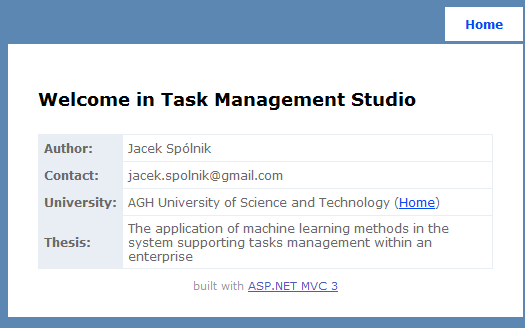
\includegraphics{anonymous_user.PNG}}
    \caption{Ekran powitania dla anonimowego u�ytkownika}
    \label{rys:anonimowyHome}
    \end{center}
\end{figure}

Kolejnym ekranem jest wspomniany ekran logowania. Pozwala on przej�� do funkcjonalnej cz�ci systemu po udanym procesie logowania. U�ytkownik jest informowany o b��dzie logowania, je�li poda nieprawid�owe dane identyfikacyjne. Dodatkowo z ekranu tego anonimowy u�ytkownik mo�e przej�� do ekranu rejestracji. Ekran ten przedstawiony jest na rysunku~\ref{rys:anonimowyLogin}.

\begin{figure}[ht]
    \begin{center}
    \fbox{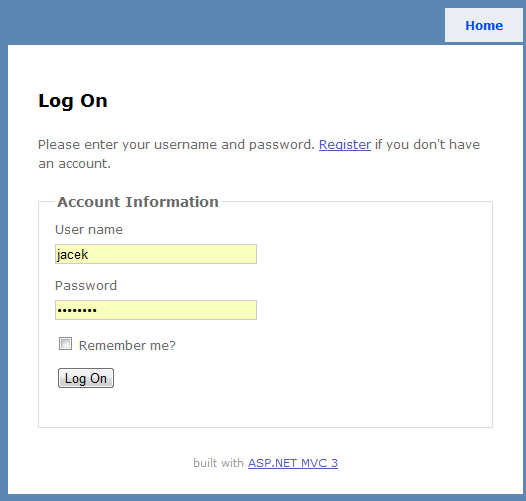
\includegraphics{anonymous_user_login.PNG}}
    \caption{Ekran logowania dla anonimowego u�ytkownika}
    \label{rys:anonimowyLogin}
    \end{center}
\end{figure}

Ostatnim ekranem dla anonimowego u�ytkownika jest ekran rejestracji. U�ytkownik podaje w nim potrzebne dane do rejestracji, po czym mo�e zalogowa� si� do systemu. Dop�ki jednak nie zostan� mu przypisane odpowiednie uprawnienia (rola), b�dzie widzia� t� sam� cz�� systemu co u�ytkownik niezalogowany poza ekranami logowania i rejestracji. Ekran rejestracji znajduje si� na rysunku~\ref{rys:anonimowyRegister}. Na ekranie wida� komunikat walidacji has�a m�wi�cy o b��dnie uzupe�nionym ha�le.

\begin{figure}[ht]
    \begin{center}
    \fbox{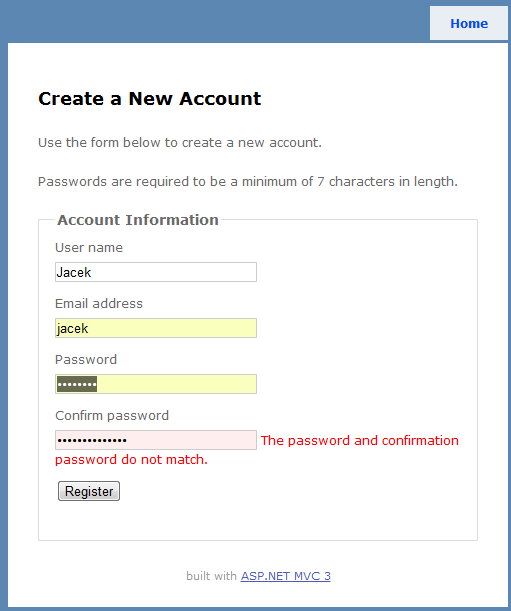
\includegraphics{anonymous_user_register.PNG}}
    \caption{Ekran rejestracji dla anonimowego u�ytkownika}
    \label{rys:anonimowyRegister}
    \end{center}
\end{figure}

%---------------------------------------------------------------------------
%---------------------------------------------------------------------------

\subsection{Administrator}

Administrator ma do dyspozycji jeden g��wny ekran, gdzie widzi detale wszystkich pracownik�w zarejestrowanych w systemie. Dodatkowo z tego ekranu mo�e przej�� do trzech innych ekran�w. Tworzenia nowego pracownika~\ref{rys:adminCreate}, usuwania istniej�cego pracownika~\ref{rys:adminDelete}, edycji danych pracownika~\ref{rys:adminEdit} oraz wy�wietlenia szczeg��w dotycz�cych pracownika~\ref{rys:adminDetails}. Cz�� ekranu g��wnego widoczna jest na rysunku~\ref{rys:adminList}.

\begin{figure}[ht]
    \begin{center}
    \fbox{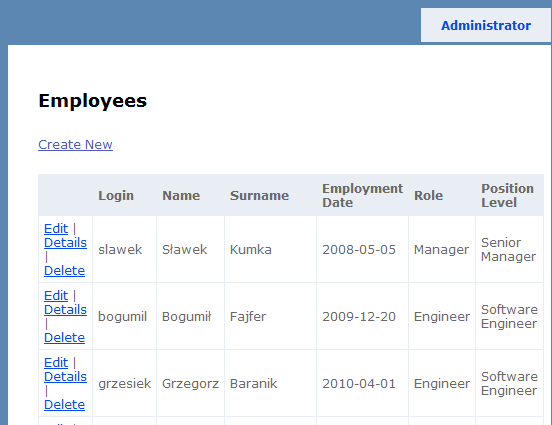
\includegraphics{admin_list.PNG}}
    \caption{Ekran g��wny dla administratora - widok na dane pracownik�w}
    \label{rys:adminList}
    \end{center}
\end{figure}

\begin{figure}[ht]
    \begin{center}
    \fbox{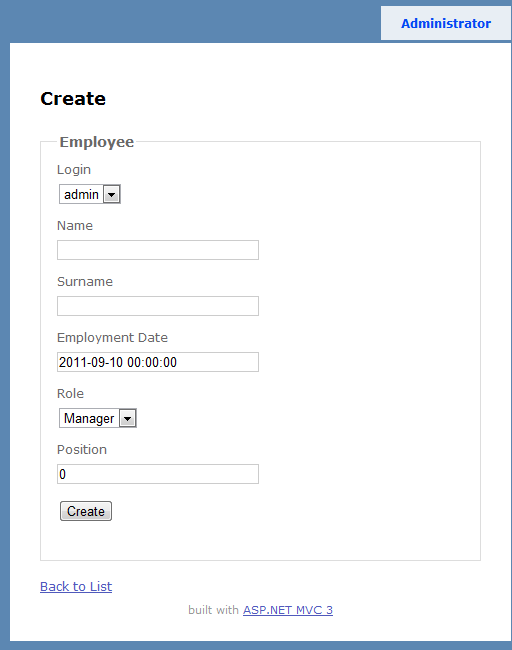
\includegraphics{admin_create.PNG}}
    \caption{Ekran tworzenia nowego pracownika}
    \label{rys:adminCreate}
    \end{center}
\end{figure}

\begin{figure}[ht]
    \begin{center}
    \fbox{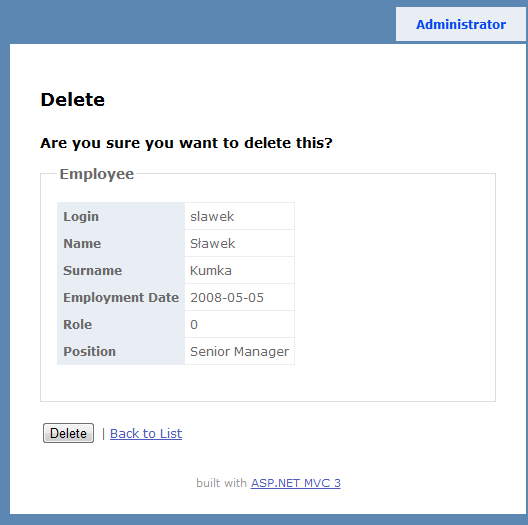
\includegraphics{admin_delete.PNG}}
    \caption{Ekran usuwania istniej�cego pracownika}
    \label{rys:adminDelete}
    \end{center}
\end{figure}

\begin{figure}[ht]
    \begin{center}
    \fbox{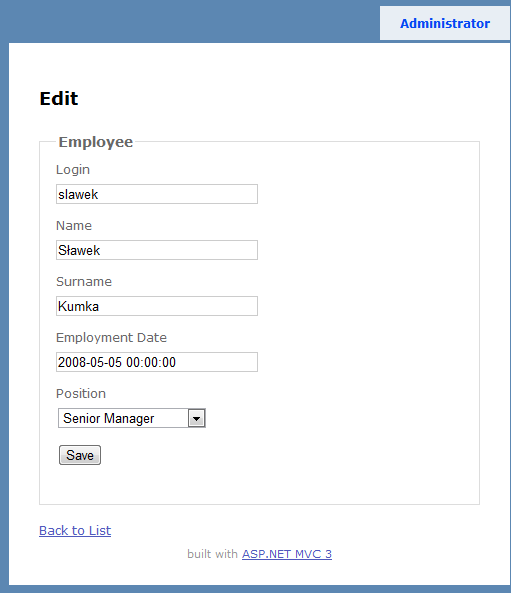
\includegraphics{admin_edit.PNG}}
    \caption{Ekran edycji danych pracownika}
    \label{rys:adminEdit}
    \end{center}
\end{figure}

\begin{figure}[ht]
    \begin{center}
    \fbox{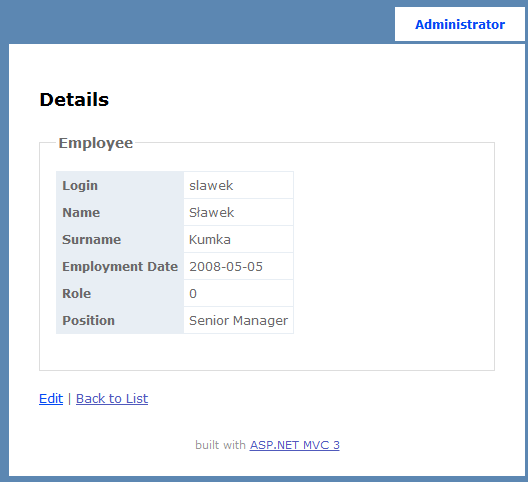
\includegraphics{admin_details.PNG}}
    \caption{Ekran wy�wietlania szczeg��w pracownika}
    \label{rys:adminDetails}
    \end{center}
\end{figure}

%---------------------------------------------------------------------------
%---------------------------------------------------------------------------

\subsection{Programista (in�ynier)}

Programista po zalogowaniu ma dost�p do dw�ch g��wnych ekran�w: ekran zada� przypisanych programi�cie oraz ekran opisuj�cy dane pracownia.

Ekran opisuj�cy dane pracownika jest stosunkowo prosty, pozwala zweryfikowa� u�ytkownikowi czy dane na jego temat zapisane w bazie firmy s� zgodne z rzeczywisto�ci�. Ekran mo�na zobaczy� na rysunku~\ref{rys:programistaAbout}.

\begin{figure}[ht]
    \begin{center}
    \fbox{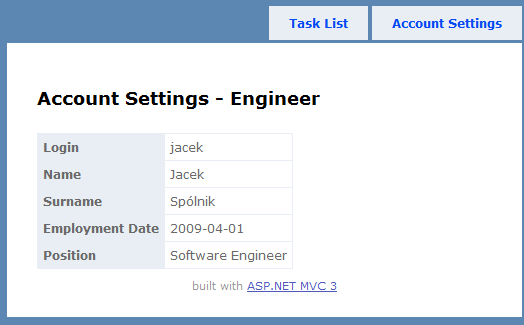
\includegraphics{developer_about.PNG}}
    \caption{Ekran informacji o zalogowanym programi�cie (in�ynierze)}
    \label{rys:programistaAbout}
    \end{center}
\end{figure}

G��wnym ekranem u�ywanym przez programist� jest ekran zada�. Ekran mo�na zobaczy� na rysunku~\ref{rys:programistaTasks}. Na ekranie jest widoczna wi�kszo�� informacji na temat poszczeg�lnych zada�. Dodatkowo z tego ekranu programista mo�e przej�� do ekranu edycji zadania~\ref{rys:programistaTaskEdit} oraz do ekranu szczeg��w zadania~\ref{rys:programistaTaskDetails}.

\begin{figure}[ht]
    \begin{center}
    \fbox{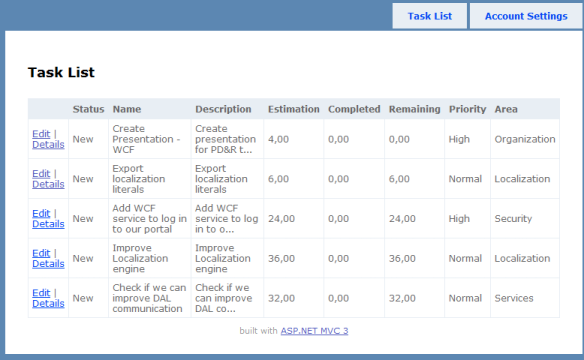
\includegraphics{developer_tasks.PNG}}
    \caption{Ekran z zadaniami przypisanymi do programisty}
    \label{rys:programistaTasks}
    \end{center}
\end{figure}

\begin{figure}[ht]
    \begin{center}
    \fbox{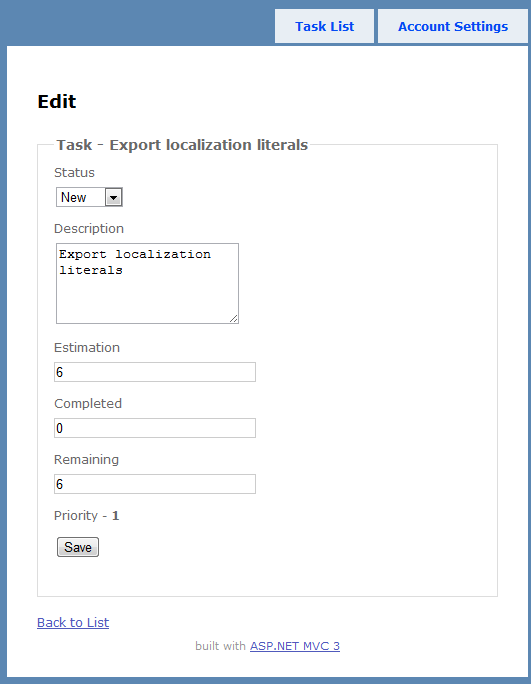
\includegraphics{developer_task_edit.PNG}}
    \caption{Ekran edycji zadania}
    \label{rys:programistaTaskEdit}
    \end{center}
\end{figure}

\begin{figure}[ht]
    \begin{center}
    \fbox{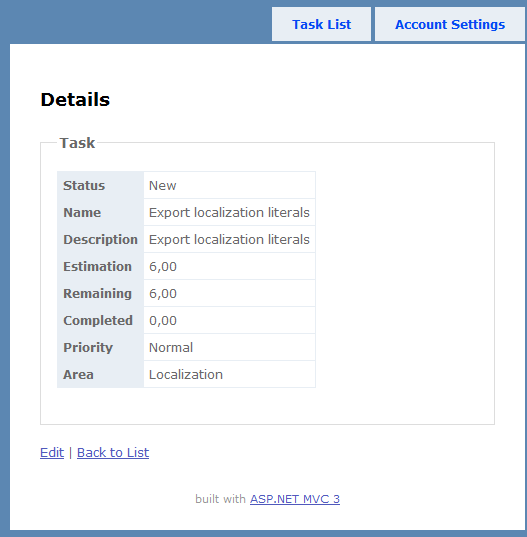
\includegraphics{developer_task_details.PNG}}
    \caption{Ekran szczeg��w zadania}
    \label{rys:programistaTaskDetails}
    \end{center}
\end{figure}

%---------------------------------------------------------------------------
%---------------------------------------------------------------------------

\subsection{Menad�er}

Menad�er, jako g��wny u�ytkownik systemu ma najwi�ksze mo�liwo�ci w samym systemie. Znaczna ilo�� ekran�w mo�liwych do przegl�dania przez menad�era nie pozwala na zamieszczenie ich wszystkich w naszej pracy. Jednak mo�emy odwo�a� si� do analogicznych ekran�w pokazywanych dla u�ytkownik�w z innymi rolami. Przyk�adowo, ekran z detalami na temat menad�era jest analogiczny do ekranu z detalami na temat programisty~\ref{rys:programistaAbout}. Ekrany do zarz�dzania wszelakimi typami obiekt�w s� analogiczne do tych, kt�re ju� widzieli�my. Usuwanie w zale�no�ci od tre�ci jest analogiczne do ekranu~\ref{rys:adminDelete}, wy�wietlanie szczeg��w obiektu do ekranu~\ref{rys:adminDetails}, edycja obiektu do ekranu~\ref{rys:adminEdit} oraz tworzenie obiektu do ekranu~\ref{rys:adminCreate}. Do om�wienia pozostaj� nam cztery specyficzne ekrany dla menad�era dotycz�ce r�nych obiekt�w.

Ekran z list� zada� prezentuje zadania przypisane do menad�era. Zadania takie czekaj� na przypisanie do konkretnego pracownika do realizacji. Bezpo�rednio z tego ekranu, kt�ry mo�na zobaczy� na rysunku~\ref{rys:managerTasks}, menad�er mo�e stworzy� nowe zadanie, doda� lub usun�� umiej�tno�� wymagan� przez zadanie, edytowa� lub przegl�da� dane zadania (mi�dzy innymi przypisa� zadanie) oraz mo�e usun�� zadanie. Dodatkowo, prezentowane okno zawiera rozszerzenie po integracji z cz�ci� algorytmiczn� w postaci dw�ch ekran�w z sugesti� najlepiej dopasowanego pracownika. Akcja \emph{Suggest Employee} u�ywa algorytmu rozszerzonego, natomiast akcja~\emph{Suggest Employee Optimized} u�ywa algorytmu podstawowego.

\begin{figure}[ht]
    \begin{center}
    \fbox{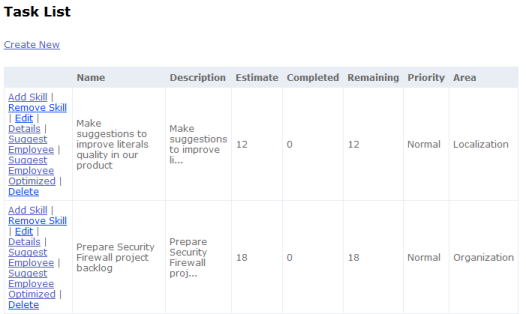
\includegraphics{manager_tasks.PNG}}
    \caption{Ekran z list� zada� przypisanych do menad�era}
    \label{rys:managerTasks}
    \end{center}
\end{figure}

Ekran z obszarami funkcjonalnymi i niefunkcjonalnymi projekt�w widoczny jest na rysunku~\ref{rys:managerAreas}. Z poziomu tego ekranu menad�er mo�e tworzy�, usuwa� i wy�wietla� szczeg�y poszczeg�lnych obszar�w.

\begin{figure}[ht]
    \begin{center}
    \fbox{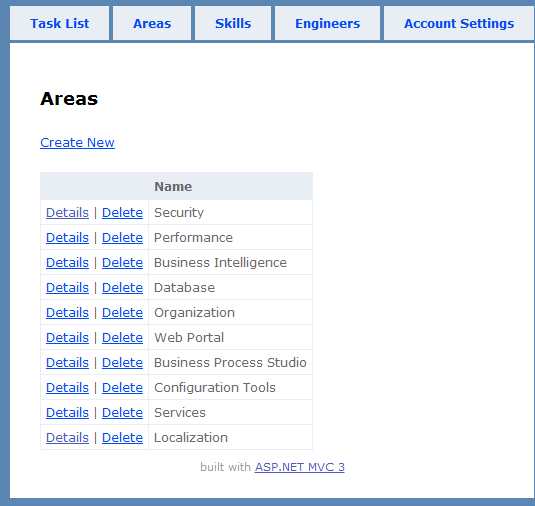
\includegraphics{manager_areas.PNG}}
    \caption{Ekran z list� obszar�w funkcjonalnych i niefunkcjonalnych}
    \label{rys:managerAreas}
    \end{center}
\end{figure}

Ekran z list� umiej�tno�ci widoczny jest na rysunku~\ref{rys:managerSkills}. Z poziomu tego ekranu menad�er mo�e tworzy�, edytowa�, usuwa� i wy�wietla� szczeg�y poszczeg�lnych umiej�tno�ci.

\begin{figure}[ht]
    \begin{center}
    \fbox{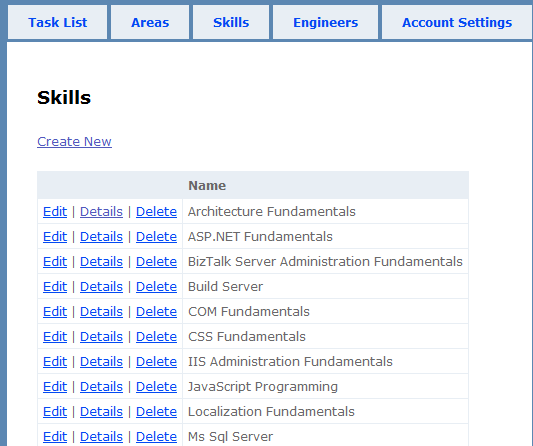
\includegraphics{manager_skills.PNG}}
    \caption{Ekran z list� umiej�tno�ci przypisywanych programistom}
    \label{rys:managerSkills}
    \end{center}
\end{figure}

Ekran z list� programist�w (in�ynier�w) widoczny jest na rysunku~\ref{rys:managerEmployees}. Ekran umo�liwia wyszukiwanie pracownika, tworzenie z jego poziomu nowego zadania, dodawania i usuwania umiej�tno�ci do pracownik�w oraz do przegl�dania danych szczeg�owych pracownik�w. Dane szczeg�owe pracownika opr�cz podstawowych danych zawieraj� list� przypisanych zada� do pracownika wraz ze szczeg�owym opisem oraz list� umiej�tno�ci przypisanych do pracownika.

\begin{figure}[ht]
    \begin{center}
    \fbox{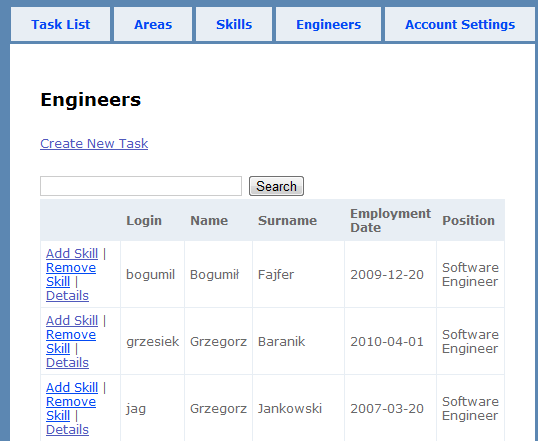
\includegraphics{manager_employees.PNG}}
    \caption{Ekran z list� programist�w}
    \label{rys:managerEmployees}
    \end{center}
\end{figure}

%\include{dodatekB}

\bibliography{bibliografia}

\end{document}
